\documentclass[11pt]{article}
\usepackage[T1]{fontenc}
\usepackage{lmodern}
\usepackage[margin=1.05in]{geometry}
\usepackage{amsmath,amssymb,amsthm,mathtools}
\usepackage{microtype}
\usepackage{tikz}
\usepackage{tabularx,booktabs}
\usetikzlibrary{arrows.meta,positioning,calc}
\usepackage{xcolor}
\usepackage{xurl}
\definecolor{linkblue}{RGB}{20,69,103}
\usepackage[colorlinks=true,linkcolor=linkblue,citecolor=linkblue,urlcolor=linkblue]{hyperref}
\hypersetup{pdftitle={Random coordinate frames and partial permutation laws},pdfauthor={OpenAI},bookmarksopen=true,bookmarksopenlevel=1,bookmarksnumbered=true}

\newtheorem{theorem}{Theorem}[section]
\newtheorem{lemma}[theorem]{Lemma}
\newtheorem{proposition}[theorem]{Proposition}
\newtheorem{corollary}[theorem]{Corollary}
\theoremstyle{definition}
\newtheorem{definition}[theorem]{Definition}
\theoremstyle{remark}
\newtheorem{remark}[theorem]{Remark}
\newcommand{\F}{\mathbb F_2}
\newcommand{\E}{\mathbb E}
\newcommand{\TV}{\mathrm{TV}}
\newcommand{\op}{\mathrm{op}}
\newcommand{\HS}{\mathrm{HS}}
\newcommand{\id}{\mathrm{id}}
\DeclareMathOperator{\tr}{tr}
\DeclareMathOperator{\Sym}{Sym}
\DeclareMathOperator{\Span}{span}
\DeclareMathOperator{\sgn}{sgn}
\newcommand{\one}{\mathbf 1}
\newcommand{\Unif}{\operatorname{Unif}}
\numberwithin{equation}{section}

\title{Random coordinate frames and partial permutation laws}
\author{OpenAI}
\date{September 26, 2026}

\makeatletter
\newcommand{\Lref}[1]{\@nameuse{companion@#1}}
\@namedef{companion@l:amplification}{2.5}
\@namedef{companion@l:branching-hs}{4.6}
\@namedef{companion@l:central-isotypic}{3.4}
\@namedef{companion@l:coefficient-lift}{4.4}
\@namedef{companion@l:degree-all-powers}{6.3}
\@namedef{companion@l:degree-inverse-first}{6.4}
\@namedef{companion@l:degree-inverse-square}{A.2}
\@namedef{companion@l:degree-inverse-ten}{A.5}
\@namedef{companion@l:degree-reciprocal-twenty}{A.1}
\@namedef{companion@l:degree-square-root-section}{A.3}
\@namedef{companion@l:degree-type-absorption}{6.5}
\@namedef{companion@l:equivariant-sixteen}{9.1}
\@namedef{companion@l:isotypic}{3.5}
\@namedef{companion@l:isotypic-alternatives}{4.3}
\@namedef{companion@l:omitted-set-transfer}{10.3}
\@namedef{companion@l:orbit-span}{3.2}
\@namedef{companion@l:single-orbit}{3.1}
\@namedef{companion@l:spectral-pruning}{10.1}
\@namedef{companion@l:tilted-entropy}{11.1}
\@namedef{companion@l:trim}{2.3}
\makeatother

\begin{document}
\maketitle
\begin{abstract}
For the Thorp shuffle on $2^d$ cards, we prove that the worst-start total-variation distance after $32800d$ physical shuffles tends to zero as $d\to\infty$. Combining our fixed-list estimate with the companion Fourier transfer improves this bound to $512d$ shuffles. These results follow from bounds on partially observed permutation laws in random coordinate frames.
\end{abstract}

\section{Introduction}
\label{sec:introduction}

A change of coordinates can relate a prescribed sequence of matching
directions to a random one. For a permutation shuffle, we identify
the joint path laws under the change of coordinates. A conditional
calculation also needs to specify what
has been revealed when the next direction is sampled. We separate these
two questions. The resulting estimates describe the laws of large
ordered lists of cards, and several ways of retaining that information
lead to convergence of the whole permutation.

Our model is the Thorp shuffle on $n=2^d$ labeled cards. Split a deck
into two equal halves, pair corresponding positions, and interleave the
pairs, choosing their orders with independent fair coins. One such
operation is one \emph{physical shuffle}. Let $q_d$ be its law as a
permutation of positions, let $U_n$ be uniform on $S_n$, and let
$\mu*\nu$ denote the law of $XY$ for independent permutations with laws
$\mu,\nu$. We use
$\|\mu-\nu\|_{\TV}=\frac12\sum_g|\mu(g)-\nu(g)|$.
A card becomes uniform after $d$ physical shuffles. The cards share the
same switches, so the law of their joint positions requires a separate
argument.

Our first complete application uses the frame, marginal, degree, and
Fourier arguments proved in this paper.

\begin{theorem}\label{thm:main}
For $n=2^d$,
\[
 \|q_d^{*(32800d)}-U_n\|_{\TV}\longrightarrow0
 \qquad(d\longrightarrow\infty).
\]
The convergence is uniform over every deterministic initial ordering
of the deck.
\end{theorem}

The lower obstruction is elementary. After $t$ physical shuffles the
process has used $tn/2$ random bits, so its support has size at most
$2^{tn/2}$ and
\[
 \|q_d^{*t}-U_n\|_{\TV}\ge1-\frac{2^{tn/2}}{n!}.
\]
At distance $1/4$ this forces
$t\ge\lceil(2/n)\log_2(3n!/4)\rceil=2d-O(1)$.
Together with Theorem~\ref{thm:main}, this shows that the mixing time
has the optimal order $d=\log_2 n$ on dyadic decks.

The proof of Theorem~\ref{thm:main} is independent of the
deterministic-coordinate companion, which proves convergence after
$1600d$ physical shuffles as $d\to\infty$
\cite[Theorem~1.1]{optimal-thorp}, and of the abstract Fourier
transfers in \cite{partial-fourier}. Later we prove that, after $256d$
shuffles, the ordered image of every fixed list of at most $7n/8$ cards
has total-variation distance $o(1)$ from a uniform injection, uniformly
over the list as $d\to\infty$. The orbit transfer gives the $2048d$ application in
Theorem~\ref{shear:thm:2048}. Combining the same marginal estimate with
the Fourier companion's isotypic estimate and its inverse-degree sum gives
the $512d$ consequence in Corollary~\ref{shear:cor:512}. The orbit
argument bounds the operator norm, while the isotypic argument bounds
the Hilbert--Schmidt norm. Later sections also prove partial laws that
retain information about histories and changing input sets.

\subsection{Coordinate frames and the first proof}

Identify positions with $V=\mathbb F_2^d$. Undoing the deterministic
rotation in each shuffle leaves independent fair switches along
successive coordinate directions. A run through all $d$ directions is
a \emph{sweep}; it costs $d$ physical shuffles. We compare this process
with switches in directions $v_1,v_2,\ldots$ such that every $d$
consecutive vectors form a basis. For a fixed sequence whose first
basis is the same ordered coordinate basis, invertible changes of position frame
identify the joint path laws. At the terminal time, the endpoint laws
agree after a specified bijection of output positions. Hence every fixed input
list has the same distance from a uniform injection in the two
descriptions. A general initial frame also relabels the inputs; the
corresponding comparison preserves the average over uniformly chosen
input lists.

This path comparison is proved after fixing the complete direction
sequence. Its intermediate maps may use future directions. The
probability calculation therefore uses a separately generated process:
after the first basis, choose the next direction uniformly outside the
span of its $d-1$ predecessors, then choose fresh switch coins. The
observation field records the input list and any independent initial
sampling, the direction prefix, and the path prefixes
of the preceding cards in the list. In this field, revealing the next
direction does not change the conditional law of the hidden card's
current position.

That card has a conditional mass on the positions not occupied by its
predecessors. A switch averages two masses when both endpoints remain
available, and transports one mass when only one endpoint remains.
The squared deviation from uniform has an exact decrement. Averaging
a fresh direction connects every pair across the hyperplane spanned by
the preceding directions with the same probability. The expected decrement
is at least the current energy times the smaller available half-count,
divided by $n$.

For the first proof we sample an omitted block of $n/64$ labels
independently of the shuffle. Its
image is contained in every available set for the complementary list.
Once the shuffle history is fixed, that image is a uniform subset, so
both sides of a specified hyperplane contain many of its positions
except with exponentially small probability. This is an unconditional
imbalance bound after the path conditioning has been removed. Since
the energy is at most one, it can be combined with the decrement even
when the energy and the imbalance event are correlated. The terminal
conditional comparison keeps the complete direction data inside total
variation until the frame identity is applied. It yields one partition
into 64 blocks for which the sum of the complementary marginal errors
after $1025d$ shuffles tends to zero.

Each complementary image list identifies a left coset of the subgroup
that permutes the omitted block. A common trimming gives one nearby law
whose relevant coset masses are capped by a fixed multiple of their
uniform values. On restricting an
irreducible representation of dimension $D$ to the product of the 64
block groups, each occurring tensor type has a factor of degree at most
$D^{1/64}$. The orbit of one vector under
that factor has controlled dimension even when the factor occurs with
large multiplicity. The transfer proof first bounds this dimension
by a finite sum of squared subgroup degrees. A local estimate for
the inverse sixteenth powers then bounds that sum, and Schur averaging
turns the coset caps into Fourier contraction. Thirty-two independent
time blocks complete the proof, with the sign representation treated
separately.

Sections~\ref{sec:prelim}--\ref{sec:frames} establish the model and
the fixed-schedule path identity. Section~\ref{sec:marginals} proves
the marginal estimate. Sections~\ref{sec:lift}, \ref{sec:degrees},
and~\ref{sec:completion} complete Theorem~\ref{thm:main} using local
representation and Fourier arguments. A reader may stop there with a
complete proof.

\subsection{Further partial laws and their uses}

Section~\ref{shear:sec:directions} reuses the conditional mass flow with
different balance and disclosure statements. A preceding transverse
switch gives an imbalance bound for every fixed input list. Independent
shears provide an explicit realization of the fresh directions, and
the deferred-column calculation identifies the coefficients that have
not yet been revealed. Sampling labels offers other balance estimates;
an arbitrary initial frame also introduces an input relabeling that
disappears after averaging over lists. Thus an average over input lists
can enter through the frame comparison or through the balance estimate.
Lemma~\ref{shear:lem:delayed-symmetry} gives a separate contraction under an earlier
conditioning time for the deterministic coordinate schedule.

Section~\ref{frames:chapter} controls exceptional trajectories in three different ways.
For a chosen partition and chosen orders of its complements, descending
removal constructs one retained measure whose complementary marginal
probabilities are capped pointwise. A stopped argument uses nested balance
events so that the tuple error includes the imbalance probability only
once. A different event, defined by the
trajectory matchings, supports an entropy inequality for every
probability law concentrated on that event. This last quantifier allows
the Fourier transfer to condition on a rare event selected from a
representation coefficient.

Section~\ref{lifts:random-marginals} uses averaged input laws in three ways: selecting one partition
for an isotypic estimate, trimming equivariant kernels while controlling
their full sign multiplicity spaces, and averaging over overlapping
omitted sets. Sections~\ref{frames:char:section} and~\ref{sec:character}
use half of the deck. When
an independent pass follows a long mixing segment, separate caps on
preimage lists control positive trace tests. When the pass comes first,
the argument repairs the two image marginals and averages one uniform
subgroup coordinate at a time. The repaired coordinates may remain
dependent.

\subsection{History and related work}

The model arose in Thorp's study of nonrandom shuffling and the game
of Faro~\cite{thorp}. Aldous and Diaconis later described the paired
shuffle and reported an informal argument for an
$O((\log n)^2)$ threshold~\cite[Section~8b, Example~(12)]{aldous-diaconis1987}.
For dyadic decks, the description by independent switches along
successive hypercube coordinates is standard~\cite{morris44}. It makes
one-card uniformity transparent, while the dependence among card
trajectories remains the obstacle to convergence of the full law.

Morris obtained an $O(d^{44})$ bound for the full deck when $n=2^d$,
combining chameleon and evolving-set ideas~\cite{morris44}. Montenegro
and Tetali sharpened that analysis to $O(d^{29})$ using spectral-profile
and evolving-set estimates~\cite[Theorems~6.14--6.15]{montenegro-tetali2006}.
Morris subsequently used entropy estimates to prove
$O((\log n)^4)$ for every even deck size~\cite{morris4} and then
$O(d^3)$ for dyadic decks~\cite{morris3}. These times count individual
physical shuffles and concern the entire permutation.

Partial-card laws were studied both as shuffle marginals and as a tool
for enciphering small domains. Morris, Rogaway and Stegers gave explicit
bounds for ordered Thorp marginals~\cite[Theorem~1]{mrs}. For dyadic
decks, Czumaj and V\"ocking proved that any prescribed list of at most
$(1-\epsilon)n$ cards mixes in $O_\epsilon((\log n)^2)$ physical layers,
for each fixed $0<\epsilon<1$, using non-Markovian couplings in the
butterfly network~\cite{CzumajVocking2014}. Czumaj's later account
identifies this as $O(\log n)$ whole butterflies~\cite[Section~1.5]{Czumaj2015}.
That paper also obtains logarithmic-depth partial mixing for other
switching networks with suitable expansion~\cite[Theorems~3.4--3.6]{Czumaj2015}.

We adapt the conditional-energy approach in the swap-or-not analysis
of Hoang, Morris and Rogaway~\cite[Section~3, Theorem~3 and Lemma~4]{hmr2014}.
Their independent uniform group keys give an unconstrained sequence of
matchings; their proof contracts a quadratic discrepancy for the next card
and compares the joint law through expected conditional errors. Dai,
Hoang and Tessaro later sharpened the combination of those squared
discrepancies through a chi-squared inequality~\cite[Section~6]{dai-hoang-tessaro2017}.
Here the next direction is constrained by its recent predecessors.
The frame identity and the chronological conditional calculation
justify that rule and its hyperplane energy estimate.

Related work connects partial information to stronger permutation
guarantees in several ways. Ristenpart and Yilek's mix-and-cut construction,
and Morris and Rogaway's sometimes-recurse construction, use partial
or separator guarantees inside recursively modified shuffles
\cite{ristenpart-yilek2013,morris-rogaway2014}. Alon and Lovett relate
uniformity for every input-output pair of a group action to Fourier
matrices of the irreducible representations occurring in that action,
and repair sufficiently accurate approximate uniformity to exact
uniformity for the action~\cite[Theorem~1.4 and Proposition~3.2]{alon-lovett2013}.
Our passage to the full symmetric group controls its irreducible Fourier
matrices from complementary coset caps for selected blocks.

\tableofcontents
\clearpage
\section{The chain and its elementary lower bound}\label{sec:prelim}

Let $d\ge1$ be an integer. Write $n=N=2^d$, let $V=\F^d$, and identify positions $0,\ldots,n-1$
with their binary strings, most significant bit first. Let $G=\Sym(V)$.
Fix card labels indexed by $V$, with card $x$ at position $x$ in
the identity state. A state $g\in G$ maps a label to its current
position, and permutations are composed as functions:
$(gh)(x)=g(h(x))$.

In one \emph{physical shuffle}, the deck is split into its top and bottom
halves, and, for $i=0,\ldots,n/2-1$, the cards at index $i$ within the
two halves occupy output positions
$2i$ and $2i+1$ in an independently chosen fair order. Thus one step
uses $n/2$ independent fair bits. In binary coordinates its action is
\begin{equation}\label{eq:physical-step}
 (x_1,x_2,\ldots,x_d)\longmapsto
 (x_2,\ldots,x_d,x_1+\xi_{(x_2,\ldots,x_d)}),
\end{equation}
where the bits indexed by the suffix are independent. This convention
counts individual physical shuffles, not sweeps of $d$ such shuffles.

Let $q_d$ be the probability law of the one-step position permutation,
and let $U$ be uniform measure on $G$. We also write $U_n$ or $U_G$
when indicating the state-space size or group is useful. The transition
kernel is $P_d(g,h)=q_d(hg^{-1})$; thus $P_d^t(g,\cdot)$ is the law
after $t$ shuffles started from $g$. For probability measures on a finite
set, we use
\[
 \|\mu-\nu\|_{\TV}
 =\frac12\sum_x|\mu(x)-\nu(x)|
 =\max_A|\mu(A)-\nu(A)|.
\]
For measures on $G$, the convolution $\mu*\nu$ is the law of $XY$, where
$X\sim\mu$ and $Y\sim\nu$ are independent. Starting from $g_0$, the law
after $t$ steps is the right translate of $q_d^{*t}$ by $g_0$.
Uniform measure is invariant under every such translation and under
left multiplication by every step. Consequently $U$ is stationary, and
\begin{equation}\label{eq:worst-state}
 \max_{g_0\in G}\|P_d^t(g_0,\cdot)-U\|_{\TV}
 =\|q_d^{*t}-U\|_{\TV}.
\end{equation}
Here and below $Y_t$ denotes the original shuffle started at the identity.
We define
\begin{equation}\label{eq:tmix}
 t_{\mathrm{mix}}(d)=
 \min\{t\in\mathbb Z_{\ge0}:\|q_d^{*t}-U\|_{\TV}\le1/4\}.
\end{equation}
Total variation is nonincreasing in $t$ by contraction under convolution.
The minimum exists for every $d\ge1$; the coordinate description in
Section~\ref{sec:frames} gives a short proof. Our estimates below give
the quantitative bound as $d$ grows.

\begin{lemma}[Support lower bound]\label{lem:lower}
For every integer $t\ge0$,
\begin{equation}\label{eq:exact-support-lower}
 \|q_d^{*t}-U\|_{\TV}\ge 1-\frac{2^{tn/2}}{n!}.
\end{equation}
Consequently,
\begin{equation}\label{eq:sharp-support-time}
 t_{\mathrm{mix}}(d)\ge
 \left\lceil\frac2n\log_2\left(\frac{3n!}{4}\right)\right\rceil
 =2d-O(1).
\end{equation}
For $0\le t\le d$,
\[
 \|q_d^{*t}-U\|_{\TV}\ge1-(e/\sqrt n)^n.
\]
In particular, the distance tends to one uniformly for integer $t\le d$,
and $t_{\mathrm{mix}}(d)\ge d$ for all sufficiently large $d$.
\end{lemma}
\begin{proof}
There are at most $2^{tn/2}$ choices of all shuffle bits, hence at most
that many possible states. If $A$ is their support, then
\[
 \|q_d^{*t}-U\|_{\TV}\ge q_d^{*t}(A)-U(A)
 \ge1-\frac{2^{tn/2}}{n!}.
\]
If this distance is at most $1/4$, the last ratio must be at least
$3/4$. Taking logarithms and then the least integer above the resulting
lower bound proves the first part of \eqref{eq:sharp-support-time}.
The integral bound
$\log(n!)\ge\int_1^n\log x\,dx=n\log n-n+1$
and $n!\le n^n$ give the asserted asymptotic lower bound. When
$t\le d$, the support ratio is at most $n^{n/2}/n!$, which is at most
$(e/\sqrt n)^n$. This proves the remaining statements.
\end{proof}

\begin{lemma}[One-card comparison]\label{lem:one-card-lower}
For a fixed initial card and an integer $0\le t<d$, its location law
has support at most $2^t$. Consequently the full permutation law has
total-variation distance at least $1-2^t/n$ from uniform, and
$t_{\mathrm{mix}}(d)\ge d$. After $d$ steps every individual card
has a uniform location.
\end{lemma}
\begin{proof}
At each step a card has at most two possible successors. Its support
therefore has at most $2^t$ positions. The uniform position law assigns
that support mass at most $2^t/n$, and passing from a full permutation
to the position of one card cannot increase total variation.
For the last assertion, undo the deterministic rotations. During the
first $d$ steps each coordinate is refreshed exactly once, with a bit
that is fair conditional on the entire previous card path. These
successive refreshed bits form a uniform binary string. Restoring the
rotation preserves uniformity.
\end{proof}

We shall use basic characteristic-zero representation theory of finite
groups: unitary realizations, orthogonal decomposition into irreducibles,
Schur's lemma, and matrix-coefficient orthogonality
\cite{etingof,sagan}. All representation spaces below are finite-dimensional
complex Hilbert spaces. For an operator $A$, $\|A\|_{\op}$ is its operator
norm and $\|A\|_{\HS}^2=\tr(A^*A)$ its squared Hilbert--Schmidt norm;
the trace is \emph{not} divided by the dimension. We prove explicitly the
dimension estimate and the passage from marginals to the full group law
that the argument requires.

\section{Changing the position frame}
\label{sec:frames}

For a nonzero vector $v\in V$, let $C_v\le G$ be the subgroup of
permutations that preserve each pair $\{x,x+v\}$ setwise. A uniform
element of $C_v$ independently swaps or fixes each of these $n/2$
pairs with equal probability. We call it a \emph{switch in direction
$v$}.

Write $e_1,\ldots,e_d$ for the standard basis of $V$, and let
\[
 R(x_1,\ldots,x_d)=(x_2,\ldots,x_d,x_1)
\]
be left cyclic rotation. Binary strings are column vectors when a
matrix acts on them. By \eqref{eq:physical-step}, one physical
shuffle is $RS_t$, where $S_t$ is uniform in $C_{e_1}$ and the
$S_t$ are independent. Thus $Y_t=RS_tY_{t-1}$, with $Y_0=\id$.
In the rotating position frame, put
\begin{equation}\label{eq:frames:cyclic}
 X_t=R^{-t}Y_t,\qquad
 Q_t=R^{-(t-1)}S_tR^{t-1}.
\end{equation}
Then $X_t=Q_tX_{t-1}$, and the $Q_t$ are independent uniform
switches in the periodic directions
$e_1,e_2,\ldots,e_d,e_1,\ldots$. Indeed, conjugation by a linear
bijection carries $C_v$ onto the matching subgroup in the image
direction, and $R^{-(t-1)}e_1=e_{1+((t-1)\bmod d)}$.

This description also proves the finite-$d$ convergence used in
Section~\ref{sec:prelim}. A sweep of $d$ layers has positive
probability of making no swaps, and positive probability of making
exactly any chosen coordinate-edge transposition. These
transpositions generate $G$, because the cube graph is connected.
Every permutation is therefore a product of finitely many sweeps.
Padding those products by identity sweeps gives a common number of
sweeps at which every permutation has positive probability. That
kernel dominates a positive multiple of $U$, so iteration proves
convergence. The rotation is the identity at the end of each sweep.

The following path identity allows a different basis in each
successive window of $d$ directions. The maps are constructed after
the complete schedule is fixed; they need not be known when their
time index is reached.

\begin{lemma}[Fixed-schedule frame identity]
\label{lem:frames}\label{shear:lem:general-frame}
Let $T\ge d$, and let $\boldsymbol\iota=(\iota_1,\ldots,\iota_d)$
be a permutation of $1,\ldots,d$. Write
$i(t)=\iota_{1+((t-1)\bmod d)}$, and let
$X^{\boldsymbol\iota}_0=\id$ and
$X^{\boldsymbol\iota}_t=Q^{\boldsymbol\iota}_t
 X^{\boldsymbol\iota}_{t-1}$, where the increments are independent
and uniform in $C_{e_{i(t)}}$.

Fix directions $v_1,\ldots,v_T$ satisfying
\begin{equation}\label{eq:frames:bases}
 (v_s,\ldots,v_{s+d-1})\text{ is a basis of }V
 \qquad(1\le s\le T-d+1).
\end{equation}
Let $Z_0=\id$, and let $Z_t$ evolve by independent uniform switches
in these directions. There are linear bijections $L_0,\ldots,L_T$,
determined by the fixed axis order and direction schedule, such that
\begin{equation}\label{shear:eq:general-frame}
 (Z_t)_{t=0}^T\overset{\mathrm{law}}=
 \bigl(L_tX^{\boldsymbol\iota}_tL_0^{-1}\bigr)_{t=0}^T,
 \qquad L_0e_{\iota_j}=v_j\quad(1\le j\le d).
\end{equation}
In particular, if $\boldsymbol\iota=(1,\ldots,d)$ and $v_j=e_j$
for $1\le j\le d$, then $L_0=I$ and
\begin{equation}\label{eq:frames:endpoint}
 Z_T\overset{\mathrm{law}}=L_TX_T=L_TR^{-T}Y_T.
\end{equation}
\end{lemma}

\begin{proof}
For $1\le s\le T-d$, the two successive bases give unique
coefficients $a_{s,t}\in\F$, $s<t<s+d$, with
\begin{equation}\label{eq:frames:recurrence}
 v_{s+d}=v_s+\sum_{s<t<s+d}a_{s,t}v_t.
\end{equation}
The coefficient of $v_s$ cannot vanish, since otherwise
$v_{s+1},\ldots,v_{s+d}$ would be dependent; over $\F$ it is
therefore one.

We construct $L_t$ so that its column selected at time $t$ has the
required value:
\begin{equation}\label{eq:frames:selected-column}
 L_{t-1}e_{i(t)}=v_t.
\end{equation}
Begin with the map $L_0$ specified in the statement. For each time
$t$, define a row $c_t$ by putting $a_{s,t}$ in column $i(s)$
whenever $1\le s\le T-d$ and $s<t<s+d$, and putting zero in every
other column. For fixed $t$ the possible $s$ lie within at most
$d-1$ consecutive times, so their coordinate indices are distinct and
differ from $i(t)$. Thus $c_te_{i(t)}=0$. Set
\begin{equation}\label{eq:frames:matrices}
 L_t=L_{t-1}(I+e_{i(t)}c_t).
\end{equation}
Each factor squares to $I$ and is invertible. It leaves the
selected column unchanged and adds prescribed multiples of that
column to the others.

Before a column's first selection no prescribed update targets it,
so \eqref{eq:frames:selected-column} holds during the first period
by the definition of $L_0$. If it is selected at time $s$ and again
at $s+d\le T$, it has value $v_s$ after the first selection. At
each intervening time $t$ it receives $a_{s,t}$ times the selected
column, whose value is $v_t$ by induction. Equation
\eqref{eq:frames:recurrence} gives its value $v_{s+d}$ before its
next selection. This proves \eqref{eq:frames:selected-column},
including an incomplete last period.

For this fixed schedule, define the transformed step shown in
Figure~\ref{fig:frames}:
\begin{equation}\label{eq:frames:transformed-step}
 \widetilde Q_t
 =L_tQ^{\boldsymbol\iota}_tL_{t-1}^{-1}
 =(L_tL_{t-1}^{-1})
   (L_{t-1}Q^{\boldsymbol\iota}_tL_{t-1}^{-1}).
\end{equation}
In \eqref{eq:frames:transformed-step}, the second factor is uniform in
$C_{v_t}$. The first is a fixed
member of that subgroup: writing $f_t=c_tL_{t-1}^{-1}$,
\[
 L_tL_{t-1}^{-1}=I+v_tf_t,\qquad f_t(v_t)=0.
\]
The map $x\mapsto x+f_t(x)v_t$ fixes or swaps each pair
$\{x,x+v_t\}$ because $f_t$ is constant on the pair. Multiplication
by it preserves the uniform law on $C_{v_t}$. Each
$\widetilde Q_t$ depends on its own independent increment
$Q^{\boldsymbol\iota}_t$, so the transformed switches are
independent. Their products telescope at every time:
\[
 \widetilde Q_t\cdots\widetilde Q_1
 =L_tQ^{\boldsymbol\iota}_t\cdots Q^{\boldsymbol\iota}_1L_0^{-1}
 =L_tX^{\boldsymbol\iota}_tL_0^{-1}.
\]
This gives the joint path identity, and the cyclic specialization
follows from \eqref{eq:frames:cyclic}.
\end{proof}

\begin{figure}[b]
 \centering
 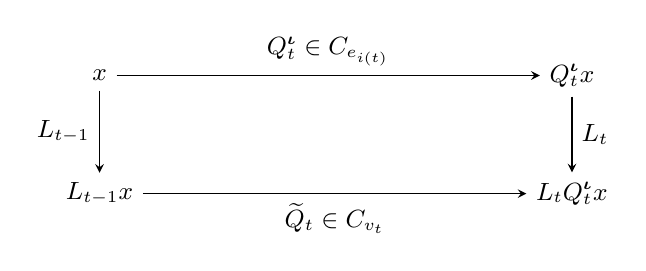
\begin{tikzpicture}[>=stealth, every node/.style={font=\small}]
  \node (a) at (0,1.5) {$x$};
  \node (b) at (6,1.5) {$Q^{\boldsymbol\iota}_tx$};
  \node (c) at (0,0) {$L_{t-1}x$};
  \node (d) at (6,0) {$L_tQ^{\boldsymbol\iota}_tx$};
  \draw[->] (a) -- node[above] {$Q^{\boldsymbol\iota}_t\in C_{e_{i(t)}}$} (b);
  \draw[->] (a) -- node[left] {$L_{t-1}$} (c);
  \draw[->] (b) -- node[right] {$L_t$} (d);
  \draw[->] (c) -- node[below] {$\widetilde Q_t\in C_{v_t}$} (d);
 \end{tikzpicture}
 \caption{One matching switch in two position frames. After the
 complete schedule is fixed, the vertical maps are deterministic
 and the lower step is an independent uniform switch in direction
 $v_t$.}
 \label{fig:frames}
\end{figure}

\begin{corollary}[Endpoint distances and the input map]
\label{cor:frames:marginals}
Under Lemma~\ref{lem:frames}, let $0\le q\le n$ and let $\pi_q$ be uniform on ordered
distinct $q$-tuples of positions. For every fixed ordered list $C$
of $q$ distinct labels,
\begin{equation}\label{eq:frames:tuple-input-map}
 \|\mathcal L(Z_T(C))-\pi_q\|_{\TV}
 =
 \|\mathcal L(X^{\boldsymbol\iota}_T(L_0^{-1}C))-\pi_q\|_{\TV}.
\end{equation}
Thus the same-list distances agree when $L_0=I$. Their averages
also agree when $C$ is sampled uniformly over ordered distinct lists,
independently of the switch process:
\begin{equation}\label{eq:frames:averaged-input-map}
 \E_C\|\mathcal L(Z_T(C)\mid C)-\pi_q\|_{\TV}
 =
 \E_C\|\mathcal L(X^{\boldsymbol\iota}_T(C)\mid C)-\pi_q\|_{\TV}.
\end{equation}
\end{corollary}
\begin{proof}
The terminal map $L_T$ is a bijection on distinct position tuples
and preserves $\pi_q$, which proves
\eqref{eq:frames:tuple-input-map}. The input map $L_0^{-1}$ also
preserves the uniform law on distinct lists, giving the averaged
identity.
\end{proof}

\begin{remark}[The schedule is fixed before the frame is constructed]
\label{rem:frames:conditioning}
If a random schedule satisfying \eqref{eq:frames:bases} is sampled
independently of the switch randomness, the lemma and corollary
apply conditionally on each complete schedule. The averaged
identity then uses a list sampled independently of that schedule
and of the switches. The maps $L_t$, including $L_0$ when the first
basis is random, may depend on directions that have not yet been
revealed. We use them only in these conditional path and endpoint
comparisons. The energy calculation next uses a separately
generated process with directions revealed in chronological order.
\end{remark}

\section{Online observations and ordinary marginals}
\label{sec:marginals}

We track the conditional location of one hidden card while revealing
the paths of earlier cards in a list. The quadratic error and the
successive comparison of conditional location laws follow the
swap-or-not approach of Hoang, Morris, and Rogaway
\cite[Section~3, Theorem~3 and Lemma~4]{hmr2014}. Here the next
direction is constrained by its recent predecessors, so we state
the information used in the calculation explicitly. The first
application below produces one partition whose complementary
marginals are all close to uniform. Later applications use the same
calculation with other sources of balance.

\subsection{A chronological law and a hidden card}

Fix an integer $T\ge0$. Let $\mathbf v=(v_1,\ldots,v_T)$ be a random schedule of nonzero
directions. Set $Z_0=\id$, and suppose that, conditional on the
complete schedule, the increments of $Z$ are independent uniform
switches in directions $v_1,\ldots,v_T$. This law can be generated
in time order: sample the next direction from its conditional law
given the preceding directions, and then use fresh fair coins on
its matching.

Let $\Xi$ be initial data independent of the joint process
$(\mathbf v,(Z_t)_{t=0}^T)$, and let
$C=(c_1,\ldots,c_q)$ be a list of distinct labels determined by
$\Xi$, with fixed length $0\le q\le n$. A fixed list corresponds to
deterministic $\Xi$; a sampled partition may be included in $\Xi$
when it determines the list. For its $j$th label define the exact
online field
\begin{equation}\label{eq:marginal-filtration}
 \mathcal F_t^{j}
 =\sigma\bigl(\Xi,v_1,\ldots,v_t,\,
        Z_s(c_i):0\le s\le t,\ i<j\bigr).
\end{equation}
Let $D_t^j$ be the positions not occupied by the observed labels
$c_1,\ldots,c_{j-1}$ at time $t$, and put $r_j=n-j+1$. Define
\begin{equation}\label{eq:marginal-energy}
 p_t^j(x)=\Pr\{Z_t(c_j)=x\mid\mathcal F_t^j\},\qquad
 \Delta_t^j=\sum_{x\in D_t^j}\left(p_t^j(x)-\frac1{r_j}\right)^2.
\end{equation}
We extend $p_t^j$ by zero outside $D_t^j$. It is a probability
vector on that set, so
$0\le\Delta_t^j=\sum_xp_t^j(x)^2-1/r_j\le1$.

For $0\le t<T$ and a feasible direction prefix write
$K_t(v)=\Pr\{v_{t+1}=v\mid v_1,\ldots,v_t\}$. Conditional on the
complete schedule, the law of the \emph{joint} permutation path
through time $t$ depends only on $v_1,\ldots,v_t$. The independence
of $\Xi$ therefore gives
\begin{equation}\label{eq:marginal-direction-factorization}
 \Pr\{Z_t(c_j)=x,\ v_{t+1}=v\mid\mathcal F_t^j\}
 =p_t^j(x)K_t(v).
\end{equation}
Indeed, the joint law of the old hidden position and observed path
prefix is the same for every completion of a fixed direction
prefix. Conditioning on that observed prefix leaves the
conditional law of the future directions unchanged. This argument
uses only path prefixes; it does not condition on future observed
paths or on further auxiliary data.

\begin{lemma}[Online averaging and cross-hyperplane contraction]
\label{lem:marginal-averaging}\label{shear:lem:energy}
In the preceding setup, for $0\le t<T$ and $1\le j\le q$,
\begin{equation}\label{eq:marginal-exact-decrement}
 \Delta_{t+1}^j=\Delta_t^j-\frac12
 \sum_{\substack{\{x,y\}\subseteq D_t^j\\y=x+v_{t+1}}}
       \bigl(p_t^j(x)-p_t^j(y)\bigr)^2
 \quad\text{almost surely},
\end{equation}
where each unordered matching edge is counted once. If $K_t$ is
uniform on the complement of an $\mathcal F_t^j$-measurable
hyperplane $J_t$, then
\begin{equation}\label{eq:marginal-cross-energy}
 \E[\Delta_t^j-\Delta_{t+1}^j\mid\mathcal F_t^j]
 \ge
 \frac{\min(|D_t^j\cap J_t|,|D_t^j\setminus J_t|)}{n}\Delta_t^j.
\end{equation}
More generally, suppose $K_t$ is uniform outside an
$\mathcal F_t^j$-measurable proper subspace $W_t$, and let $J_t$
be an $\mathcal F_t^j$-measurable hyperplane containing $W_t$.
Then the same right side with denominator $2n$ is a valid lower
bound.
\end{lemma}
\begin{proof}
Fix $j$ and omit its superscript. By
\eqref{eq:marginal-direction-factorization}, revealing $v_{t+1}$
does not update the old hidden-card law $p_t$. Given
$\mathcal F_t$ and this direction, the matching edges incident to
observed cards are known. Their next positions reveal exactly the
fresh coins on those edges. Those coins are independent of the old
hidden position, so their revelation also leaves $p_t$ unchanged;
all other edge coins remain independent and fair.

An edge containing two positions of $D_t$ averages their two
masses. An edge containing exactly one position of $D_t$ transports
its mass to the unique position on that edge unoccupied by observed
cards after the switch. Edges with no available position carry no
hidden mass. These rules give the conditional vector at the exact
field $\mathcal F_{t+1}$ in \eqref{eq:marginal-filtration}. They
also transport the uniform vector on $D_t$ to the uniform vector
on $D_{t+1}$. Transport preserves squared error, while averaging
two masses reduces it by
$\frac12(p_t(x)-p_t(y))^2$. This proves the exact identity.

For the expectation, split $D_t=D^0\cup D^1$ across $J_t$ and put
$z_x=p_t(x)-1/r_j$, $u=|D^0|$, and $w=|D^1|$. Since $\sum z_x=0$,
\begin{equation}\label{shear:eq:bipartite-form}
 \sum_{x\in D^0,y\in D^1}(z_x-z_y)^2
 =w\sum_{D^0}z_x^2+u\sum_{D^1}z_y^2
     +2\left(\sum_{D^0}z_x\right)^2
 \ge\min(u,w)\sum_{D_t}z_x^2.
\end{equation}
Every cross pair has matching probability $2/n$ in the hyperplane
case. Combining this with the factor $1/2$ in the exact decrement
proves \eqref{eq:marginal-cross-energy}. In the proper-subspace
case, every cross difference lies outside $W_t$ and has probability
$1/(n-|W_t|)\ge1/n$; discard the other eligible pairs to obtain
the denominator $2n$. The calculation covers an empty side.
The algebraic identity \eqref{shear:eq:bipartite-form} holds for
any real centered vector; a later use for another vector must also
identify its averaging rule.
\end{proof}

The loss bound and a balance estimate will be used at different
levels of conditioning. Let $0\le\gamma\le1$. If the conditional expected loss
$\E[\Delta_t^j-\Delta_{t+1}^j\mid\mathcal F_t^j]$ is at least
$\gamma\Delta_t^j$ off an event $B_t\in\mathcal F_t^j$ and is
always nonnegative, then $\Delta_t^j\le1$ gives
\begin{equation}\label{eq:marginal-balance-recurrence}
 \E\Delta_{t+1}^j
 \le(1-\gamma)\E\Delta_t^j+\gamma\Pr(B_t).
\end{equation}
Thus an unconditional bound on $\Pr(B_t)$ suffices; no bound
conditional on the observed paths is asserted.

\subsection{From hidden cards to an ordinary tuple law}

Let $\pi_q$ be uniform on ordered distinct $q$-tuples of positions,
and let $U_D$ be uniform on a nonempty set $D$. For any tuple law
$\nu=\mathcal L(Y_1,\ldots,Y_q)$,
\begin{equation}\label{eq:marginal-sequential-tv}
 \|\nu-\pi_q\|_{\TV}
 \le\sum_{j=1}^q\E_\nu
 \left\|
 \mathcal L(Y_j\mid Y_1,\ldots,Y_{j-1})
 -U_{V\setminus\{Y_1,\ldots,Y_{j-1}\}}
 \right\|_{\TV}.
\end{equation}
This sequential comparison appears in
\cite[Appendix~A, Lemma~2]{mrs}; an earlier distinct-tuple form is
\cite[Section~5.3, Lemma~12]{morris-exclusion2006}.
For completeness, at the $j$th step insert the law that first
draws the actual $(j-1)$-coordinate prefix of $\nu$ and then
appends a uniform available position. Its distance from the
$j$-coordinate marginal of $\nu$ is the $j$th summand above.
Applying the same extension kernel to $\pi_{j-1}$ gives $\pi_j$
and contracts total variation. The triangle inequality and
induction prove \eqref{eq:marginal-sequential-tv}. Every
expectation is under the actual prefix law.

\begin{lemma}[Terminal data and an ordinary tuple law]
\label{shear:lem:tuple}
In the preceding setup let $\Lambda$ be terminal data that
determine the complete direction schedule, and suppose $\Xi$ is
independent of $(\Lambda,(Z_t)_{t=0}^T)$. For every
$1\le j\le q$ and every $x\in V$, assume
that its online terminal vector is also the conditional hidden
law after these data and the complete predecessor paths are known:
\begin{equation}\label{eq:marginal-terminal-identification}
 \Pr\{Z_T(c_j)=x\mid
       \Lambda,\Xi,\,
       Z_s(c_i):0\le s\le T,\ i<j\}
 =p_T^j(x)\quad\text{almost surely}.
\end{equation}
Then
\begin{equation}\label{shear:eq:tuple-bound}
 \E_{\Lambda,\Xi}
 \|\mathcal L(Z_T(C)\mid\Lambda,\Xi)-\pi_q\|_{\TV}
 \le\frac12\sum_{j=1}^q
       \sqrt{(n-j+1)\E\Delta_T^j}.
\end{equation}
All expectations are under the actual joint law of the data, list,
and process. If $\E\Delta_T^j\le a_T$ for every $j$, the right
side is at most $q\sqrt n\,\sqrt{a_T}/2$. For $q=0$ both sides are
zero.
\end{lemma}
\begin{proof}
For fixed $\Lambda,\Xi$, apply
\eqref{eq:marginal-sequential-tv}. At index $j$ use the coarser
field
\[
 \mathcal H_j
 =\sigma(\Lambda,\Xi,Z_T(c_1),\ldots,Z_T(c_{j-1})).
\]
The tower property and \eqref{eq:marginal-terminal-identification}
give
$\Pr\{Z_T(c_j)=x\mid\mathcal H_j\}
 =\E[p_T^j(x)\mid\mathcal H_j]$.
The set $D_T^j$ is $\mathcal H_j$-measurable, so Jensen's
inequality for the $\ell^1$ norm compares both vectors to the
same uniform law $U_{D_T^j}$. Cauchy--Schwarz gives
\[
 \|p_T^j-U_{D_T^j}\|_{\TV}
 \le\frac12\sqrt{(n-j+1)\Delta_T^j}.
\]
Consequently, almost surely in the terminal data and initial data,
\begin{equation}\label{eq:marginal-conditional-tuple}
 \|\mathcal L(Z_T(C)\mid\Lambda,\Xi)-\pi_q\|_{\TV}
 \le\frac12\sum_{j=1}^q
 \E\!\left[\sqrt{(n-j+1)\Delta_T^j}\,\middle|\,\Lambda,\Xi\right].
\end{equation}
Averaging and applying Cauchy--Schwarz once more proves the lemma.
\end{proof}

When $\Lambda=\mathbf v$, the field on the left of
\eqref{eq:marginal-terminal-identification} is exactly
$\mathcal F_T^j$, so that hypothesis is automatic. If $\Lambda$
contains further shear or functional data, the identification
requires an additional path-law argument. We will prove that
argument where those data are introduced; their disclosure is
separate from the chronological averaging above.

\subsection{A sampled omitted block}

For the local full-group proof, set
\begin{equation}\label{eq:marginal-constants}
 k=64,\qquad m=\frac{n}{k},\qquad
 \alpha=\frac1{4k},\qquad T=(1+16k)d=1025d,
\end{equation}
and assume $d\ge6$. Put
\begin{equation}\label{eq:marginal-error}
 b_n=2\left(\frac{2}{3^{3/4}}\right)^m,\qquad
 \varepsilon_n=\frac{n^{3/2}}2\sqrt{e^{-4d}+b_n}.
\end{equation}
For a labeled partition $\mathcal M=(M_1,\ldots,M_k)$ of $V$
into $m$-element blocks, let $\delta_a(\mathcal M)$ be the
distance of the time-$T$ images of $V\setminus M_a$ under the
physical shuffle from the uniform distinct tuple law. Any fixed
ordering of these labels gives the same distance.

\begin{proposition}[One partition with nearly complete marginals]
\label{prop:marginals}
There is a deterministic labeled partition
$\mathcal M=(M_1,\ldots,M_k)$ into blocks of size $m$ for which
\begin{equation}\label{eq:marginal-partition}
 \sum_{a=1}^k\delta_a(\mathcal M)
 \le k\varepsilon_n=o(1)\qquad(d\longrightarrow\infty).
\end{equation}
\end{proposition}

\begin{proof}
Use $v_i=e_i$ for $1\le i\le d$. For $d\le t<T$ put
\begin{equation}\label{eq:marginal-hyperplane}
 J_t=\Span\{v_{t-d+2},\ldots,v_t\}
\end{equation}
and choose $v_{t+1}$ uniformly in $V\setminus J_t$, with fresh
direction randomness. Every $d$ successive directions form a
basis. Conditional on the complete schedule, use independent fair
switches to form $Z$. Independently choose $\mathcal M$ uniformly
among labeled equal-size partitions. For a fixed $a$, let $\Xi$
be this partition and let $C$ be any deterministic ordering of
$V\setminus M_a$, with $q=n-m$. This is the online setup above.

For each hidden index $j$, the available set contains the positions
of all omitted labels:
\begin{equation}\label{eq:marginal-permanent-holes}
 Z_t(M_a)\subseteq D_t^j.
\end{equation}
Write $D_t^{j,0}=D_t^j\cap J_t$ and
$D_t^{j,1}=D_t^j\setminus J_t$. If
$J_t^0=J_t$ and $J_t^1=V\setminus J_t$, then
\[
 \left\{\min_i|D_t^j\cap J_t^i|<m/4\right\}
 \subseteq
 \left\{\min_i|Z_t(M_a)\cap J_t^i|<m/4\right\}.
\]
Fix the direction and switch history through time $t$, but not
$\mathcal M$. This fixes $Z_t$ and $J_t$, while $Z_t(M_a)$ is a
uniform $m$-subset of $V$.

For a uniform $m$-subset and a fixed half of $V$, let $X$ be its
count in that half. View the subset as an ordered sample without
replacement. A specified set of $\ell$ sampled indices all lie
in the half with probability at most $2^{-\ell}$. If $I_i$ are
the membership indicators, expansion gives
\[
 \E3^X=\E\prod_{i=1}^m(1+2I_i)
 \le\sum_{A\subseteq\{1,\ldots,m\}}2^{|A|}2^{-|A|}=2^m.
\]
If one half contains fewer than $m/4$ sampled points, the other
contains more than $3m/4$. Markov's inequality and a union bound
therefore yield, for $d\le t<T$,
\begin{equation}\label{eq:marginal-balance}
 \Pr\{\min(|D_t^{j,0}|,|D_t^{j,1}|)<m/4\}
 \le2\frac{2^m}{3^{3m/4}}=b_n.
\end{equation}
This bound averages the independent partition and the shuffle; it
is not a concentration assertion conditional on the observed paths.

Off the event in \eqref{eq:marginal-balance}, the conditional loss
in \eqref{eq:marginal-cross-energy} is at least
$\alpha\Delta_t^j$. Its loss is always nonnegative. Applying
\eqref{eq:marginal-balance-recurrence} gives
\begin{equation}\label{eq:marginal-recursion}
 \E\Delta_{t+1}^j
 \le(1-\alpha)\E\Delta_t^j+\alpha b_n.
\end{equation}
Starting with $\Delta_d^j\le1$ and iterating for $T-d=16kd$
steps, we obtain, uniformly in $a,j$,
\begin{equation}\label{eq:marginal-terminal-energy}
 \E\Delta_T^j\le(1-\alpha)^{T-d}+b_n
 \le e^{-4d}+b_n.
\end{equation}

Let $\widetilde\delta_a(\mathbf v,\mathcal M)$ be the auxiliary
tuple distance conditional on the complete schedule and partition.
Use Lemma~\ref{shear:lem:tuple} with $\Lambda=\mathbf v$.
Its terminal identification is automatic, since
$\mathcal F_T^j$ already contains the complete schedule and
predecessor paths. Equations
\eqref{shear:eq:tuple-bound} and
\eqref{eq:marginal-terminal-energy} give
\begin{equation}\label{eq:marginal-averaged-tuple}
 \E_{\mathbf v,\mathcal M}
 \widetilde\delta_a(\mathbf v,\mathcal M)
 \le\frac{n^{3/2}}2\sqrt{e^{-4d}+b_n}
 =\varepsilon_n.
\end{equation}
The schedule remains inside the distance on the left.

For every fixed schedule and partition, choose
$\boldsymbol\iota=(1,\ldots,d)$ in Lemma~\ref{lem:frames}.
The first directions are $v_j=e_j$, so $L_0=I$. Corollary
\ref{cor:frames:marginals}, followed by the terminal rotation,
therefore gives the same-list identity
\begin{equation}\label{eq:marginal-frame-transfer}
 \widetilde\delta_a(\mathbf v,\mathcal M)=\delta_a(\mathcal M).
\end{equation}
The frame maps enter only this fixed-schedule endpoint comparison.
Summing \eqref{eq:marginal-averaged-tuple} over $a$ now gives
$\E_{\mathcal M}\sum_a\delta_a(\mathcal M)\le k\varepsilon_n$.
At least one deterministic partition attains this average bound.
Finally,
$n^{3/2}e^{-2d}=\exp((\tfrac32\log2-2)d)\to0$, while
$2/3^{3/4}<1$ makes $b_n$ exponentially small in $n$.
Thus $\varepsilon_n\to0$.
\end{proof}

\section{From large marginals to a finite degree sum}
\label{sec:lift}

Proposition~\ref{prop:marginals} gives one partition for which the
complementary image laws have small total error. We first express those
image laws as coset laws and condition on one event that bounds all their
coset densities. We then turn these bounds into a finite sum of squared
degrees of representations of the block groups. The next section will
estimate that sum by counting tableaux.

Throughout this section, \(U_G\) denotes the uniform probability measure on
a finite group \(G\). For a subgroup \(H\), we use the standard convention
that \(gH\) is a \emph{left coset}. Its elements are obtained from \(g\) by
multiplication on the right by elements of \(H\). If \(\mu\) is a probability
measure on \(G\), write \(\mu_H\) for its pushforward to the set \(G/H\) of
left cosets. Thus
\[
  \mu_H(gH)=\mu(gH),
  \qquad (U_G)_H(gH)=\frac{|H|}{|G|}.
\]

For the shuffle application, take $X=V$, set $T=1025d$ and
$\mu=q_d^{*T}$, and use the deterministic partition
$M_1,\ldots,M_k$ supplied by Proposition~\ref{prop:marginals},
with $k=64$ and $|M_a|=n/k$. Let $H_a$ permute $M_a$ and fix
$X\setminus M_a$ pointwise.
A permutation maps each reference label to its current position. Two maps
\(g,g'\) agree on \(X\setminus M_a\) exactly when
\(g^{-1}g'\in H_a\), or equivalently \(g'\in gH_a\). Thus the ordered
images of the cards outside \(M_a\) identify the coset \(gH_a\)
bijectively. Uniform measure on permutations induces uniform measure on
these ordered distinct images. The marginal distances in
Proposition~\ref{prop:marginals} are consequently exactly the coset
distances \(\delta_a\) for the trimming lemma below, and
\(\sum_a\delta_a=o(1)\).

\begin{lemma}[Simultaneous trimming]
\label{lem:trim}
Let \(H_1,\ldots,H_k\) be subgroups of a finite group \(G\), and let
\(\mu\) be a probability measure on \(G\). Put
\[
  \delta_a=\|\mu_{H_a}-(U_G)_{H_a}\|_{\TV},
  \qquad \delta=\sum_{a=1}^k\delta_a.
\]
If \(\delta<1/2\), there is a set \(E\subseteq G\), of removed mass
\(\varepsilon=\mu(G\setminus E)\le 2\delta\), such that the conditional
probability measure \(\bar\mu=\mu(\,\cdot\mid E)\) satisfies
\begin{equation}
\label{eq:lift:trim}
  \|\bar\mu-\mu\|_{\TV}=\varepsilon,
  \qquad
  \bar\mu(gH_a)
  \le \frac{2}{1-\varepsilon}\frac{|H_a|}{|G|}
  \quad(g\in G,\ 1\le a\le k).
\end{equation}
In particular, if \(\delta\le 1/4\), the last density bound is at most
\(4|H_a|/|G|\).
\end{lemma}

\begin{proof}
For each \(a\), call a coset \(C\in G/H_a\) bad if
\(\mu(C)>2U_G(C)\), and let \(B_a\) be the union of its bad cosets.
The identity expressing total variation as the sum of positive excesses
gives
\[
  \mu(B_a)
  \le 2\sum_{\substack{C\in G/H_a\\ \mu(C)>2U_G(C)}}
                 \bigl(\mu(C)-U_G(C)\bigr)
  \le 2\delta_a.
\]
Take \(E=G\setminus\bigcup_a B_a\). The union bound yields
\(\varepsilon\le 2\delta<1\), so conditioning is well defined. On \(E\),
the mass of \(\bar\mu\) exceeds that of \(\mu\) by total amount
\(\varepsilon\); on the complement, its mass is zero. This proves the
total-variation equality in \eqref{eq:lift:trim}.

Fix a coset \(C\in G/H_a\). If it is bad for this subgroup, then
\(C\cap E=\varnothing\). Otherwise,
\[
  \bar\mu(C)
  =\frac{\mu(C\cap E)}{1-\varepsilon}
  \le \frac{\mu(C)}{1-\varepsilon}
  \le \frac{2U_G(C)}{1-\varepsilon}.
\]
The same estimate therefore holds for every coset in every one of the
\(k\) systems. If \(\delta\le 1/4\), then
\(1-\varepsilon\ge 1/2\), giving the last assertion.
\end{proof}

We now convert the coset bounds into control of averages of representation
matrices. For a mass function \(a:G\to\mathbb C\) and a unitary
representation \(\rho\), define its Fourier matrix by
\[
  \widehat a(\rho)=\sum_{g\in G}a(g)\rho(g).
\]
Probability and subprobability measures are identified with their mass
functions. For a finite group \(H\), write \(\widehat H\) for the set of
equivalence classes of its complex irreducible representations.

When an irreducible representation of \(G\) is restricted to the product
of the block groups, each irreducible summand is a tensor product of one
representation from each group. If the full representation has dimension
\(D\), each such tensor product has dimension at most \(D\), so at least
one factor has degree at most \(D^{1/k}\). The following proposition
measures the cost of these small factors by a finite sum. Its proof shows
why each equivalence class of a subgroup representation contributes only
the square of its degree even when it occurs with large multiplicity.

\begin{proposition}[Coset densities and squared subgroup degrees]
\label{prop:lift:orbit-sum}
Let a finite set \(X\) be partitioned into \(k\ge1\) nonempty sets
\(M_1,\ldots,M_k\), and put \(G=\Sym(X)\). Let \(H_a\) be the subgroup
permuting \(M_a\) and fixing \(X\setminus M_a\) pointwise. Suppose that a
probability measure \(\nu\) on \(G\) satisfies, for some \(B\ge 1\),
\begin{equation}
\label{eq:lift:coset-cap}
  \nu(gH_a)\le B\frac{|H_a|}{|G|}
  \qquad(g\in G,\ 1\le a\le k).
\end{equation}
Then every irreducible complex unitary representation \(\rho\) of \(G\), of
dimension \(D\), satisfies
\begin{equation}
\label{eq:lift:orbit-sum}
  \|\widehat\nu(\rho)\|_{\op}^2
  \le \frac{B}{D}\sum_{a=1}^k
       \sum_{\substack{\pi\in\widehat H_a\\\dim\pi\le D^{1/k}}}
                    (\dim\pi)^2.
\end{equation}
The block sizes need not be equal.
\end{proposition}

\begin{proof}
Because the blocks are disjoint, their subgroups form the direct product
\(H=H_1\times\cdots\times H_k\) inside \(G\). By complete reducibility
and the irreducible-representation theorem for finite direct products,
the restriction of \(\rho\) to \(H\) is an orthogonal sum of isotypic
spaces of the form
\begin{equation}
\label{eq:lift:restriction}
  (V_{\pi_1}\otimes\cdots\otimes V_{\pi_k})
       \otimes \mathcal A_{\boldsymbol\pi}.
\end{equation}
Here \(\pi_a\) is an irreducible representation of \(H_a\), and
\(\mathcal A_{\boldsymbol\pi}\) is a multiplicity space on which \(H\)
acts trivially. These are the usual characteristic-zero representation
facts; see, for example, \cite{sagan,etingof}.

For every type \(\boldsymbol\pi\) that occurs, its tensor-product
dimension is at most \(D\). Consequently some index \(a\) satisfies
\(\dim\pi_a\le D^{1/k}\). Assign each entire isotypic space in
\eqref{eq:lift:restriction} to one such index, choosing the least one
in case of a tie. Grouping the assigned spaces yields an orthogonal
decomposition
\[
  V_\rho=E_1\oplus\cdots\oplus E_k.
\]
Each \(E_a\) is invariant under \(H\), and every irreducible of \(H_a\)
appearing in \(E_a\) has dimension at most \(D^{1/k}\). The multiplicities
in these restrictions are unrestricted.

For this fixed representation, put
\[
  r_a=\sum_{\substack{\pi\in\widehat H_a\\\dim\pi\le D^{1/k}}}
                (\dim\pi)^2.
\]
Fix \(u_a\in E_a\), and set
\[
  W_a=\Span\{\rho(h)u_a:h\in H_a\}.
\]
We first bound this single-vector orbit span. Regroup all copies of each
\(H_a\)-irreducible, including copies coming from different \(H\)-types,
into a single \(H_a\)-isotypic space. In such an isotypic
space \(V_\pi\otimes\mathcal A_\pi\), with \(b=\dim\pi\), the group
acts by \(\pi(h)\otimes\id\). If \(v\) is the projection of \(u_a\)
to this space, its orbit span is contained in the image of the linear map
\[
  \operatorname{End}(V_\pi)\longrightarrow
          V_\pi\otimes\mathcal A_\pi,
  \qquad Q\longmapsto (Q\otimes\id)v.
\]
That image has dimension at most \(b^2\), independently of
\(\dim\mathcal A_\pi\). Each inequivalent \(H_a\)-type contributes only
once. Summing over the different isotypic spaces gives the finite bound
\begin{equation}
  \dim W_a\le r_a
  =\sum_{\substack{\pi\in\widehat H_a\\\dim\pi\le D^{1/k}}}
                         (\dim\pi)^2.
\label{eq:lift:orbit-dimension}
\end{equation}

Let \(\Pi_a\) be the orthogonal projection onto \(W_a\). The subspace
\(W_a\) is \(H_a\)-invariant, and therefore
\(\rho(gh)W_a=\rho(g)W_a\) for \(h\in H_a\). For each vector \(z\),
the nonnegative function
\[
  g\longmapsto
       \|\Pi_{\rho(g)W_a}z\|^2
\]
is thus constant on each left coset \(gH_a\). The coset bound
\eqref{eq:lift:coset-cap} implies
\begin{equation}
\label{eq:lift:projection-comparison}
  \E_{g\sim\nu}\|\Pi_{\rho(g)W_a}z\|^2
  \le B\E_{g\sim U_G}\|\Pi_{\rho(g)W_a}z\|^2.
\end{equation}
The uniform average of these projections is
\[
  Q_a=\frac1{|G|}\sum_{g\in G}\rho(g)\Pi_a\rho(g)^*.
\]
It commutes with every \(\rho(g)\). Schur's lemma makes it a scalar
multiple of \(\id\), and its trace is \(\dim W_a\). Hence
\begin{equation}
\label{eq:lift:schur-average}
  Q_a=\frac{\dim W_a}{D}\id,
  \qquad
  \E_{g\sim U_G}\|\Pi_{\rho(g)W_a}z\|^2
       =\frac{\dim W_a}{D}\|z\|^2.
\end{equation}

Since \(\rho(g)u_a\in\rho(g)W_a\), Cauchy--Schwarz, first for
expectation and then in the representation space, gives
\begin{align}
  |\langle z,\widehat\nu(\rho)u_a\rangle|^2
  &\le \E_{g\sim\nu}|\langle z,\rho(g)u_a\rangle|^2 \notag\\
  &\le \|u_a\|^2
           \E_{g\sim\nu}\|\Pi_{\rho(g)W_a}z\|^2 \notag\\
  &\le \frac{Br_a}{D}\|u_a\|^2\|z\|^2,
\label{eq:lift:component-bound}
\end{align}
where the last line uses
\eqref{eq:lift:orbit-dimension}--\eqref{eq:lift:schur-average}.
For an arbitrary \(u=\sum_a u_a\), sum the square-root form of this
estimate and apply Cauchy--Schwarz in the index \(a\):
\begin{align*}
 |\langle z,\widehat\nu(\rho)u\rangle|
 &\le \sqrt{\frac{B}{D}}\,\|z\|
           \sum_{a=1}^k\sqrt{r_a}\,\|u_a\|\\
 &\le \sqrt{\frac{B}{D}\sum_{a=1}^k r_a}\,\|z\|
           \left(\sum_{a=1}^k\|u_a\|^2\right)^{1/2}\\
 &=\sqrt{\frac{B}{D}\sum_{a=1}^k r_a}\,\|z\|\,\|u\|.
\end{align*}
The last equality uses the orthogonality of the \(E_a\). Taking the
supremum over unit vectors \(u,z\) and squaring proves
\eqref{eq:lift:orbit-sum}. The argument includes zero components and
one-dimensional representations; in dimension one the displayed sum
does not provide decay.
\end{proof}

\section{An elementary bound on representation degrees}
\label{sec:degrees}

Proposition~\ref{prop:lift:orbit-sum} reduced the Fourier estimate to a
finite sum of squared degrees of small representations of each block
group. We now bound that sum. For integers $s,D,k\ge1$ and a
group $H\cong S_s$, we have
\begin{align}
 \sum_{\substack{\pi\in\widehat H\\\dim\pi\le D^{1/k}}}(\dim\pi)^2
 &=\sum_{\substack{\pi\in\widehat H\\\dim\pi\le D^{1/k}}}
       (\dim\pi)^{18}(\dim\pi)^{-16}\notag\\
 &\le D^{18/k}\sum_{\pi\in\widehat H}(\dim\pi)^{-16}.
\label{eq:degrees:truncated-sum}
\end{align}
Thus a uniform bound on the sum of inverse sixteenth powers of degrees will
control every block size in the preceding proposition. We also prove that
the sum tends to zero after the trivial and sign representations are
removed. That second statement will control the full-group Fourier sum
in the completion.

Recall that the complex irreducible representations of $S_s$ are indexed
by partitions $\lambda\vdash s$, and that their degrees $f^\lambda$ count
standard Young tableaux of shape $\lambda$. Such a tableau fills the
diagram with $1,\ldots,s$, increasing along every row and column. The
partitions $(s)$ and $(1^s)$ afford the trivial and sign representations,
respectively; transposing a tableau gives
$f^{\lambda'}=f^\lambda$.
These are the classical Specht-module and standard-tableau facts
\cite{sagan,etingof}. Liebeck and Shalev prove the stronger estimate
$\sum_{\lambda\vdash s}(f^\lambda)^{-u}=2+O_u(s^{-u})$
as $s\to\infty$, for every fixed $u>0$
\cite[Theorems~1.1 and~2.6]{liebeck-shalev2004}.
The following elementary proof at exponent $16$ keeps this application
independent of that stronger estimate; it uses only the tableau facts just
recalled.

\begin{lemma}[Summability of inverse degrees]
\label{lem:degrees}
There is an absolute finite constant
\begin{equation}
  C_0:=\sup_{s\ge 1}\sum_{\lambda\vdash s}(f^\lambda)^{-16}<\infty.
  \label{eq:degrees:uniform}
\end{equation}
Moreover,
\begin{equation}
  \sum_{\substack{\lambda\vdash s\\
                  \lambda\notin\{(s),(1^s)\}}}
       (f^\lambda)^{-16}\longrightarrow 0
       \qquad\text{as }s\longrightarrow\infty.
  \label{eq:degrees:vanishing}
\end{equation}
The excluded partitions are interpreted as a set, so when $s=1$ only
the single partition $(1)$ is excluded.
\end{lemma}

\begin{proof}
We first record two elementary counting observations.
If a diagram has first row of length $a$ and exactly $b$ boxes below it,
where $0\le b\le a$, then
\begin{equation}
  f^\lambda\ge \binom{a}{b}.
  \label{eq:degrees:tableau-construction}
\end{equation}
This is the tableau construction of Liebeck and Shalev
\cite[Lemma~2.1]{liebeck-shalev2004}, with their parameters $n=a+b$ and
$k=b$. To see it directly, place $1,\ldots,b$ in the first $b$ boxes of
the first row.
Choose any $b$ labels from $\{b+1,\ldots,a+b\}$ for the boxes below
that row, and put them in increasing row-major order: read rows from
top to bottom, and each row from left to right. Fill the rest of the
first row increasingly with the remaining labels. Every box below
the first row lies in one of its first $b$ columns. Its top-row
predecessor therefore has a label at most $b$, while all lower labels
are larger than $b$. Row-major filling respects both row and column
inequalities within the lower diagram, so this is a standard tableau.
Different choices of lower labels give different tableaux. When $b=0$
the construction is the unique tableau of a single row.

Also, if $\mu$ is a Young subdiagram of $\lambda$, every standard
tableau of $\mu$ extends to one of $\lambda$: retain its labels and
fill the remaining boxes in row-major order with the successive
larger labels. Because a Young subdiagram is closed under moving up
and left, all required predecessors have already been filled.
Consequently,
\begin{equation}
  f^\lambda\ge f^\mu.
  \label{eq:degrees:extension}
\end{equation}

Write $p(t)$ for the number of partitions of $t$. For $t\ge 1$,
regarding a partition as an ordered composition gives
\begin{equation}
  p(t)\le 2^{t-1}\le 2^t,
  \label{eq:degrees:partition-count}
\end{equation}
since a composition is specified by cuts in the $t-1$ gaps between
$t$ successive units. We set $p(0)=1$.

For a partition $\lambda\vdash s$, put
\[
  L=\max\{\lambda_1,\lambda'_1\},\qquad h=s-L.
\]
After transposing if necessary, assume its first row has length $L$.
This does not change its degree. The case $h=0$ consists precisely of
the row and column partitions, which are excluded from
\eqref{eq:degrees:vanishing}. We divide the other diagrams into three
classes.

\smallskip
\noindent\textit{A long first row or column: $1\le h\le s/3$.}
For fixed $h$, there are at most $2p(h)$ original shapes: after a
possible transpose, the diagram below the first row is a partition
of $h$. By \eqref{eq:degrees:tableau-construction},
\[
  f^\lambda\ge\binom{s-h}{h}
  \ge \left(\frac{s-h}{h}\right)^h\ge 2^h.
\]
Here the middle inequality follows by writing
$\binom{a}{b}=\prod_{j=0}^{b-1}(a-j)/(b-j)$ and bounding each factor
below by $a/b$ when $a\ge b\ge1$.
Thus the total inverse-degree contribution with a given $h$ is at most
\[
  2\cdot 2^h\binom{s-h}{h}^{-16}
  \le 2\cdot 2^{-15h}.
\]
For each fixed positive $h$, the binomial coefficient tends to infinity
with $s$. The displayed geometric majorant is summable over $h$.
Extending a contribution by zero when $h>s/3$, dominated convergence
for this series shows that the total contribution of this class tends
to zero.

\smallskip
\noindent\textit{Intermediate width: $h>s/3$ and $L\ge s/8$.}
Here $L<2s/3$, so $h>L/2$. Set $b=\lfloor L/2\rfloor$ and take
the subdiagram $\mu$ consisting of the whole first row and the first
$b$ boxes below it in row-major order. There are enough boxes because
$h\ge b$, and an initial segment of row-major order in the lower
diagram is again a Young diagram. Applying
\eqref{eq:degrees:extension} and
\eqref{eq:degrees:tableau-construction} gives
\[
  f^\lambda\ge \binom{L}{\lfloor L/2\rfloor}
  \ge \frac{2^L}{L+1}
  \ge \frac{2^{s/8}}{s+1}.
\]
The central binomial coefficient is the largest of the $L+1$
coefficients whose sum is $2^L$. Using
\eqref{eq:degrees:partition-count}, the total contribution of this
class is therefore at most
\begin{equation}
  2^s\left(\frac{s+1}{2^{s/8}}\right)^{16}
  =(s+1)^{16}2^{-s}\longrightarrow0.
  \label{eq:degrees:intermediate}
\end{equation}

\smallskip
\noindent\textit{Small width and height: $L<s/8$.}
Number row and column indices starting at $1$, and group boxes by
their index sum. There are at most $2L-1$ nonempty such diagonals.
Fill the diagonals in increasing index-sum order, assigning the next
available consecutive labels to each diagonal in any order. Every
row or column predecessor has a strictly smaller index sum, so every
such filling is a standard tableau. If the nonempty diagonal sizes
are $u_1,\ldots,u_q$, then
\[
  f^\lambda\ge \prod_{j=1}^q u_j!
  \ge \prod_{j=1}^q 2^{u_j-1}
  =2^{s-q}\ge 2^{3s/4}.
\]
We used $u!\ge2^{u-1}$ for integers $u\ge1$, and
$q\le2L-1<s/4$. The inverse-degree contribution of this class is
at most
\begin{equation}
  2^s\bigl(2^{3s/4}\bigr)^{-16}
  =2^{-11s}\longrightarrow0.
  \label{eq:degrees:small-width}
\end{equation}

These three classes cover all partitions except the row and column,
so they prove \eqref{eq:degrees:vanishing}. For every $s\ge2$ those
two partitions are distinct and each has degree $1$. The complete
sum in \eqref{eq:degrees:uniform} consequently tends to $2$ as
$s\to\infty$. For each fixed positive $s$ it is a finite sum of
positive terms, since there are finitely many partitions and every
degree is a positive integer. The tail of this convergent sequence
is bounded, and its finitely many initial values have a finite
maximum. This proves \eqref{eq:degrees:uniform}, including $s=1$,
where the complete sum is $1$.
\end{proof}

In representation notation, the uniform conclusion of the lemma is
\begin{equation}
\label{eq:lift:degree-constant}
 C_0=\sup_{s\ge1}\sum_{\pi\in\widehat{S_s}}(\dim\pi)^{-16}<\infty.
\end{equation}
We can now finish the transfer from bounded coset densities to Fourier
decay. The bound is uniform over the block sizes because $C_0$ is uniform
over all positive integers $s$.

\begin{corollary}[From bounded coset densities to Fourier decay]
\label{prop:lift}
Let a finite set $X$ be partitioned into $k>18$ nonempty sets
$M_1,\ldots,M_k$, and put $G=\Sym(X)$. Let $H_a$ be the subgroup that
permutes $M_a$ and fixes $X\setminus M_a$ pointwise. Suppose that a
probability measure $\nu$ on $G$ satisfies, for some $B\ge1$,
\[
 \nu(gH_a)\le B\frac{|H_a|}{|G|}
 \qquad(g\in G,\ 1\le a\le k).
\]
Then every irreducible complex unitary representation $\rho$ of $G$, of
dimension $D$, satisfies
\begin{equation}
\label{eq:lift:general-fourier}
 \|\widehat\nu(\rho)\|_{\op}
 \le\sqrt{kBC_0}\,D^{-(1-18/k)/2}.
\end{equation}
Here $C_0$ is the absolute constant of Lemma~\ref{lem:degrees}. The block
sizes need not be equal.
\end{corollary}

\begin{proof}
For every $a$, the group $H_a$ is isomorphic to $S_{|M_a|}$. Hence
\eqref{eq:degrees:truncated-sum} and Lemma~\ref{lem:degrees} give
\[
 \sum_{\substack{\pi\in\widehat H_a\\\dim\pi\le D^{1/k}}}(\dim\pi)^2
 \le C_0D^{18/k}.
\]
In the orbit construction of Proposition~\ref{prop:lift:orbit-sum}, this
recovers $\dim W_a\le C_0D^{18/k}$, and the component bound
\eqref{eq:lift:component-bound} becomes
\[
 |\langle z,\widehat\nu(\rho)u_a\rangle|^2
 \le BC_0D^{-1+18/k}\|u_a\|^2\|z\|^2.
\]
Substituting the displayed degree bound into
\eqref{eq:lift:orbit-sum} yields
\[
 \|\widehat\nu(\rho)\|_{\op}^2
 \le kBC_0D^{-1+18/k}.
\]
Taking square roots proves \eqref{eq:lift:general-fourier}.
\end{proof}

\section{Completion of the mixing bound}\label{sec:completion}

Return to $G=\Sym(V)$ for $n=2^d$. We now pass from the operator estimate
to the full permutation law.
Use the Fourier convention from Section~\ref{sec:lift}, and write
$D_\rho$ for the dimension of an irreducible unitary representation
$\rho$. Our convolution convention gives
$\widehat{\mu*\nu}(\rho)=\widehat\mu(\rho)\widehat\nu(\rho)$.
The following Plancherel bound is the classical Fourier method used by
Diaconis and Shahshahani~\cite{DiaconisShahshahani1981}. We keep the
full matrix form because the shuffle law need not be central, and we
record the normalization explicitly.

\begin{lemma}[The full-group variation bound]\label{lem:plancherel}
For any probability measure $\nu$ on $G$,
\begin{equation}\label{eq:plancherel-tv}
 4\|\nu-U\|_{\TV}^2
 \le\sum_{\rho\ne\mathrm{triv}}D_\rho
       \|\widehat\nu(\rho)\|_{\HS}^2,
\end{equation}
where the sum contains one representative of each nontrivial irreducible
equivalence class.
\end{lemma}
\begin{proof}
Cauchy--Schwarz bounds the left side by
$|G|\sum_g|\nu(g)-|G|^{-1}|^2$.
For any real function $a$ on $G$, expansion and the regular-character
identity give
\begin{align*}
 \sum_\rho D_\rho\Bigl\|\sum_g a(g)\rho(g)\Bigr\|_{\HS}^2
 &=\sum_{g,h}a(g)a(h)
   \sum_\rho D_\rho\tr\bigl(\rho(h)^*\rho(g)\bigr)\\
 &=|G|\sum_g a(g)^2.
\end{align*}
Apply this to $a(g)=\nu(g)-|G|^{-1}$. The trivial coefficient vanishes;
uniform averaging in every nontrivial irreducible is zero. These facts
give \eqref{eq:plancherel-tv}.
\end{proof}

\begin{lemma}[Fair sign]\label{lem:fair-sign}
For every $d\ge1$ and every integer $t\ge1$,
$\widehat{q_d^{*t}}(\sgn)=0$. If a probability measure $\nu$ is
$\varepsilon$ away from $q_d^{*t}$ in total variation, then
$|\widehat\nu(\sgn)|\le2\varepsilon$. If instead
$0\le\xi\le q_d^{*t}$ has mass $m$, then
$|\widehat\xi(\sgn)|\le1-m$.
\end{lemma}
\begin{proof}
Condition on every switch bit except one in the final physical shuffle.
Changing that bit composes the output permutation with a transposition,
so its two possible signs are opposite and equally likely. The
expectation of sign is therefore zero. The two perturbation estimates
follow by summing against a function of absolute value one; their
respective $\ell^1$ differences are $2\varepsilon$ and $1-m$.
\end{proof}

\begin{proof}[Proof of Theorem~\ref{thm:main}]
Fix
$k=64$ and let $d\ge6$ grow. Put $T=1025d$ and
$\mu=q_d^{*T}$. Proposition~\ref{prop:marginals} supplies a partition
of the labels into $k$ sets of size $m=n/k$ for which the sum of the
complementary marginal errors tends to zero. Lemma~\ref{lem:trim}
therefore applies with their sum at most $1/4$ for all sufficiently large
$d$. It supplies a probability measure $\bar\mu$ such that
\begin{equation}\label{eq:final-trim}
 \|\bar\mu-\mu\|_{\TV}=o(1),\qquad
 \bar\mu(gH_a)\le4\frac{|H_a|}{|G|}\quad(g\in G,\ 1\le a\le k).
\end{equation}
Here $H_a$ permutes the $a$th label block and fixes all other labels.
Corollary~\ref{prop:lift} gives,
simultaneously for every irreducible $\rho$ of dimension $D$,
\begin{equation}\label{eq:final-op}
 \|\widehat{\bar\mu}(\rho)\|_{\op}
 \le A D^{-23/64},\qquad A=\sqrt{4\cdot64\,C_0},
\end{equation}
where $C_0$ is the absolute constant in Lemma~\ref{lem:degrees}.

Take $\ell=32$, a fixed number independent of $d$. Operator-norm
submultiplicativity and $\|B\|_{\HS}\le\sqrt D\|B\|_{\op}$ show that
the contribution of the nontrivial, nonsign representations to the right
side of \eqref{eq:plancherel-tv}, for $\nu=\bar\mu^{*\ell}$, is at most
\begin{align}
 \sum_{\rho\ne\mathrm{triv},\sgn}
       D\|\widehat{\bar\mu}(\rho)^\ell\|_{\HS}^2
 &\le A^{64}\sum_{\rho\ne\mathrm{triv},\sgn}
       D^{2-64(23/64)}\notag\\
 &=A^{64}\sum_{\rho\ne\mathrm{triv},\sgn}D^{-21}=o(1).
 \label{eq:final-degree-sum}
\end{align}
The last conclusion follows from Lemma~\ref{lem:degrees}, since
$D^{-21}\le D^{-16}$ for $D\ge1$. Neither diagonalizability nor normality
of the Fourier matrices is needed here.

The sign representation has dimension one, so
\eqref{eq:final-op} alone gives no decay. Lemma~\ref{lem:fair-sign}
shows that $\widehat\mu(\sgn)=0$ and therefore
\[
 |\widehat{\bar\mu}(\sgn)|
 \le2\|\bar\mu-\mu\|_{\TV}=o(1).
\]
Its contribution after $\ell$ factors is therefore $o(1)$ as well.
Together with Lemma~\ref{lem:plancherel} and
\eqref{eq:final-degree-sum}, this proves
$\|\bar\mu^{*32}-U\|_{\TV}=o(1)$.

Convolution by a probability measure contracts total variation.
Replacing the factors one at a time and using \eqref{eq:final-trim} gives
\[
 \|\mu^{*32}-U\|_{\TV}
 \le32\|\mu-\bar\mu\|_{\TV}
       +\|\bar\mu^{*32}-U\|_{\TV}=o(1).
\]
Successive independent $T$-step blocks of the original shuffle have law
$\mu$, so $\mu^{*32}=q_d^{*32800d}$. Equation~\eqref{eq:worst-state}
makes this conclusion uniform over the initial ordering. In particular
the distance is at most $1/4$ for all sufficiently large $d$, as required.
\end{proof}

The constants were chosen to leave room in two simple estimates: the
hidden-card contraction must overcome the number of sequential marginal
comparisons, and the fixed convolution count must overcome the Fourier
dimension weights. No optimal leading constant or cutoff statement is
asserted. Together with the support lower bound, the result gives
mixing order $\Theta(d)$.

\paragraph{Further partial-permutation laws.}
Theorem~\ref{thm:main} is complete with the frame, omitted-block, orbit,
and tableau arguments above. The remaining sections compare estimates for
each fixed list with estimates averaged over lists. They then examine what
can be retained after stopping or conditioning on trajectory events and
develop Fourier and character transfers for those forms of partial
information.

\section{Fixed input laws and independent shears}
\label{shear:sec:directions}

The local proof obtained balance by sampling one omitted block.
For an arbitrary fixed input list, a previous switch supplies
balance instead: it crosses the two halves relevant to the next
direction, and the intervening switches preserve those halves.
This gives an ordinary tuple law for every fixed list. We then
record an independent shear realization of fresh directions
and several estimates that retain an average over inputs.
The realization will also control which auxiliary data may be
disclosed in the later history arguments.

We use $N=n=2^d$ and the coordinate process
$X^{\boldsymbol\iota}$ of Lemma~\ref{lem:frames}, where
$\boldsymbol\iota=(\iota_1,\ldots,\iota_d)$ is any ordering of
the standard axes and $i(s)=\iota_{1+((s-1)\bmod d)}$. Thus
\begin{equation}\label{shear:eq:coordinate-chain}
 X^{\boldsymbol\iota}_0=\id,\qquad
 X^{\boldsymbol\iota}_s=h_sX^{\boldsymbol\iota}_{s-1},\qquad
 h_s\sim U_{C_{e_{i(s)}}}
\end{equation}
with independent increments. The order $(1,\ldots,d)$ gives the
rotating-frame chain $X$; its physical permutation is $R^sX_s$.
Other starting phases and the reversed order are included by
choosing another $\boldsymbol\iota$.

\subsection{Balance for every fixed list}

We will use the following elementary concentration estimates.
\begin{lemma}[Concentration estimates]\label{lem:concentration}
Let $X_1,\ldots,X_r$ be independent random variables in $[0,1]$
and put $S=\sum_iX_i$. For $a\ge0$ and $r\ge1$,
\[
 \Pr(S-\E S\ge a),\quad\Pr(S-\E S\le-a)\le e^{-2a^2/r}.
\]
More generally, if $(M_j)_{j=0}^r$ is a real martingale whose
increments have absolute value at most $c_j$, either tail at
distance $a$ is at most
$\exp[-a^2/(2\sum_jc_j^2)]$ when the denominator is positive.
If all $c_j$ vanish, the martingale is constant. In particular,
if $X$ counts the points of a uniform $m$-subset in a fixed half
of a finite set of even size, then
\[
 \Pr(X<m/4)\le e^{-m/32}\qquad(m\ge1).
\]
\end{lemma}
\begin{proof}
For a variable $Z$ in an interval of length $b$, put
$\psi(s)=\log\E e^{sZ}$. Its second derivative is the variance
under the exponentially tilted law, at most $b^2/4$. Integrating
from $\psi(0)=0$ and $\psi'(0)=\E Z$ gives
$\E e^{s(Z-\E Z)}\le e^{s^2b^2/8}$. Multiplication and
minimization in $s$ prove the independent-variable bound. The
conditional version, with interval length $2c_j$, gives
$\E e^{s(M_r-M_0)}\le e^{s^2\sum_jc_j^2/2}$ and the martingale
bound. These are the exponential-moment arguments underlying the
inequalities of Hoeffding and Azuma
\cite{hoeffding1963,azuma1967}.

Expose a uniform subset in a uniform random order and form the
Doob martingale for its final half-count. The expected final count
changes by at most one at each draw: completions following two
possible next draws can be coupled by exchanging those points.
The initial expectation is $m/2$. Use $r=m$, $c_j=1$, and
$a=m/4$.
\end{proof}

For the fixed-list estimate, generate $Z$ directly as in
Section~\ref{sec:marginals}: its first $d$ directions are
$v_j=e_{\iota_j}$, and for $s>d$ choose $v_s$ uniformly outside
the hyperplane
\begin{equation}\label{shear:eq:hyperplane}
 W_s=\Span(v_{s-d+1},\ldots,v_{s-1}).
\end{equation}
Given the complete schedule, the switches are independent and
uniform. Every $d$ consecutive directions form a basis. For a
fixed input list, take deterministic initial data $\Xi$ in
\eqref{eq:marginal-filtration}.

\begin{lemma}[Balance after the previous transverse switch]
\label{shear:lem:fixed-balance}
Fix any $\ell<N$ observed labels, and put $m=N-\ell$. For $s>d$,
let $D_{s-1}$ be their available positions just before step $s$.
Then
\begin{equation}\label{shear:eq:fixed-balance}
 \Pr\{\min(|D_{s-1}\cap W_s|,|D_{s-1}\setminus W_s|)<m/4\}
 \le2e^{-m/8}.
\end{equation}
The probability averages the observed paths; it is not
conditional on them.
\end{lemma}
\begin{proof}
Fix the complete direction schedule. The direction $v_{s-d}$
crosses the two cosets of $W_s$, because the $d$ directions
starting at $s-d$ form a basis. The intervening directions lie
in $W_s$ and preserve each coset.

Condition on the observed configuration immediately before step
$s-d$. Let $a$ be the number of matching pairs with two available
positions and $b$ the number with one, so $m=2a+b$. Immediately
after this crossing switch, the available count on either chosen
side is $a+\operatorname{Bin}(b,1/2)$, using $b$ independent fair
coins. Its mean is $m/2$. If $b>0$, Lemma~\ref{lem:concentration}
bounds a deviation of at least $m/4$ by
$2\exp(-2(m/4)^2/b)\le2e^{-m/8}$; if $b=0$ the count is exactly
$m/2$. The intervening switches preserve the count. Remove the
conditioning to obtain the claim.
\end{proof}

\begin{proposition}[Uniform large-marginal estimates]
\label{shear:prop:fixed-marginal}
Let $L\ge2$ be a fixed integer dividing $N$, and let
$0\le q\le N-N/L$. For every ordered list $C$ of $q$ distinct
labels, every periodic ordering $\boldsymbol\iota$ of the standard
axes, and every integer $T\ge d$,
\begin{equation}\label{shear:eq:general-fixed-marginal}
 \|\mathcal L(X^{\boldsymbol\iota}_T(C))-\pi_q\|_{\TV}
 \le\frac{N^{3/2}}2
 \left(e^{-(T-d)/(4L)}+2e^{-N/(8L)}\right)^{1/2}.
\end{equation}
The same bound holds for $(X^{\boldsymbol\iota}_T)^{-1}(C)$.
For the physical shuffle and its inverse, the corresponding
position laws satisfy the same bound.

The following choices used below give distance at most
$N^{3/2}\sqrt{a_T}/2$:
\begin{align}
 L=8,\quad T=256d:&\quad
 a_T=(31/32)^{255d}+64e^{-N/64},
 \label{shear:eq:256-marginal}\\
 L=8,\quad T=257d:&\quad
 a_T=e^{-8d}+2e^{-N/64},
 \label{shear:eq:257-marginal}\\
 L=32,\quad T=2049d:&\quad
 a_T=e^{-16d}+256e^{-N/256}.
 \label{shear:eq:2049-marginal}
\end{align}
Each of these three substituted bounds tends to zero as
$d\to\infty$, uniformly in the list and axis order. The last
energy bound is $o(N^{-4})$.
\end{proposition}
\begin{proof}
For a successive hidden-card problem, its number $m$ of
available positions is at least $N/L$. Off the event in
\eqref{shear:eq:fixed-balance}, Lemma~\ref{shear:lem:energy}
gives conditional expected loss at least
$\gamma\Delta_t$, where $\gamma=1/(4L)$. The loss is always
nonnegative. Equation~\eqref{eq:marginal-balance-recurrence}
therefore gives, for $t\ge d$,
\begin{equation}\label{shear:eq:fixed-recursion}
 \E\Delta_{t+1}\le(1-\gamma)\E\Delta_t
       +2\gamma e^{-N/(8L)}.
\end{equation}
Starting from $\Delta_d\le1$ yields
$\E\Delta_T\le(1-\gamma)^{T-d}+2e^{-N/(8L)}$.
Apply Lemma~\ref{shear:lem:tuple} with terminal data
$\Lambda=\mathbf v$. For every complete schedule, the first
basis is $(e_{\iota_1},\ldots,e_{\iota_d})$, so $L_0=I$ in
Lemma~\ref{lem:frames}. The same-list equality
\eqref{eq:frames:tuple-input-map} transfers the conditional
tuple bound to $X^{\boldsymbol\iota}$, giving
\eqref{shear:eq:general-fixed-marginal}.

Each switch is an involution. Reversing the independent factors
therefore identifies $(X^{\boldsymbol\iota}_T)^{-1}$ with a
coordinate chain whose first axis is $i(T)$ and whose periodic
order is reversed. This is another permitted ordering, so the
same estimate applies. The relation $Y_T=R^TX_T$ transfers the
forward physical law by an output bijection. Its inverse is
$X_T^{-1}R^{-T}$; the input bijection only changes the fixed
list, and the bound is uniform in that list.

For \eqref{shear:eq:256-marginal}, weaken the additive term in
\eqref{shear:eq:fixed-recursion} to $2e^{-N/64}$ and sum the
geometric series, giving the factor $64$. At $257d$ keep the
sharper recurrence and use $(31/32)^{256d}\le e^{-8d}$.
More generally, at $T=(1+64L)d$, the weakened additive term
$2e^{-N/(8L)}$ gives $e^{-16d}+8Le^{-N/(8L)}$, yielding
\eqref{shear:eq:2049-marginal}. These rates dominate the factor
$N^3$ in the squared tuple bound, and $e^{-16d}=o(N^{-4})$.
\end{proof}

\subsection{An independent shear realization}

The fixed-list proof above uses the directly generated direction
process. The next construction couples a process with a triangular
first basis and the same later uniform-complement rule to a
coordinate chain with the same fixed inputs. It also proves the
conditional path identity needed when the auxiliary shear entries
are retained at terminal time.

\begin{lemma}[Independent shear realization]\label{shear:lem:keys}
Fix an axis order $\boldsymbol\iota$ and a horizon $T\ge d$. Independently
of the increments in \eqref{shear:eq:coordinate-chain}, choose
independent fair bits $b_{sj}$ for $j\ne i(s)$, put
$b_{s,i(s)}=0$, and write $\Lambda$ for all these entries. Set
\[
 S_s=I+e_{i(s)}b_s,\qquad
 A_0=I,\quad A_s=A_{s-1}S_s,\qquad
 v_s=A_{s-1}e_{i(s)},\qquad
 Z_s=A_sX^{\boldsymbol\iota}_s.
\]
Conditional on $\Lambda$, the increments of $Z$ are independent
uniform switches in directions $v_s$. More precisely, if
$\mathsf P_{v_1,\ldots,v_t}$ is the product-switch path law
through time $t$ starting at the identity, then
\begin{equation}\label{shear:eq:prefix-factorization}
 \mathcal L((Z_s)_{s=0}^t\mid\Lambda)
 =\mathsf P_{v_1,\ldots,v_t}\qquad(0\le t\le T).
\end{equation}
Every $d$ consecutive directions form a basis. For $s>d$,
conditional on $v_1,\ldots,v_{s-1}$, the next direction is
uniform on $V\setminus W_s$, with $W_s$ as in
\eqref{shear:eq:hyperplane}. This law is unchanged by additionally
observing any part of the virtual path prefix through time $s-1$.
\end{lemma}
\begin{proof}
The map $S_s$ is an involution in $C_{e_{i(s)}}$, because
$b_se_{i(s)}=0$. The increment of $Z$ is
\[
 A_{s-1}(S_sh_s)A_{s-1}^{-1}.
\]
For fixed $\Lambda$, the factors $S_sh_s$ are independent and
uniform in their coordinate matching groups. Conjugation gives
the asserted product-switch law, including the joint prefix
identity \eqref{shear:eq:prefix-factorization}.

Extend $i(s)$ periodically beyond $T$ and define the deterministic
next-read time of a column by
\[
 \tau(s,j)=\min\{t>s:i(t)=j\}\qquad(j\ne i(s)).
\]
Right multiplication by $S_s$ leaves the selected column
unchanged and adds $b_{sj}v_s$ to column $j$. Thus the direction
at a column's first read, for $t\le d$, is
\[
 v_t=e_{i(t)}+\sum_{1\le u<t}b_{u,i(t)}v_u.
\]
These first $d$ directions form a triangular basis. At later
reads,
\begin{equation}\label{shear:eq:key-recurrence}
 v_t=v_{t-d}+\sum_{t-d<u<t}b_{u,i(t)}v_u\qquad(t>d).
\end{equation}
In either display the coefficients used at time $t$ are exactly
the entries whose next-read time is $t$. Inductively, all earlier
directions are functions only of entries with next-read time
less than $t$. The batch read at $t$ is therefore independent
and fair conditional on those directions. The recurrence also
shows inductively that every consecutive $d$ directions form a
basis. For $t>d$, its fresh $d-1$ coefficients make $v_t$
uniform on
$v_{t-d}+W_t=V\setminus W_t$.

Finally, \eqref{shear:eq:prefix-factorization} says that the
entire virtual path prefix and $\Lambda$ are conditionally
independent given the direction prefix. Hence observing any
portion of that path prefix cannot reveal the fresh batch that
determines the next direction.
\end{proof}

For initial data $\Xi$ independent of $(\Lambda,(Z_s)_{s=0}^T)$
and determining the observed list, the joint prefix factorization
gives, for every $0\le t\le T$, $1\le j\le q$, and $x\in V$,
\begin{equation}\label{shear:eq:terminal-factorization}
 \Pr\{Z_t(c_j)=x\mid\Lambda,\Xi,\,
              Z_s(c_i):0\le s\le t,\ i<j\}
 =p_t^j(x),
\end{equation}
where $p_t^j$ uses the chronological field
\eqref{eq:marginal-filtration}. At $t=T$ this is precisely the
terminal identification required by Lemma~\ref{shear:lem:tuple}.
For $t<T$ it concerns only predecessor path prefixes through
$t$; conditioning on their future paths requires the separate
path-cylinder argument in Section~\ref{frames:chapter}.
The next direction is averaged in the smaller chronological field
before $\Lambda$ is disclosed.

The coupling also preserves every fixed input list conditionally
on the shears:
\begin{equation}\label{shear:eq:fixed-list-frame}
 \|\mathcal L(Z_T(C)\mid\Lambda)-\pi_q\|_{\TV}
 =\|\mathcal L(X^{\boldsymbol\iota}_T(C))-\pi_q\|_{\TV}.
\end{equation}
Indeed, $X^{\boldsymbol\iota}$ is independent of $\Lambda$ and
$Z_T=A_TX^{\boldsymbol\iota}_T$, with $A_T$ a bijection on
outputs. Here $A_0=I$ although the first directions are generally
triangular combinations of the coordinate axes. This same-input
identity is a feature of the shear realization; the arbitrary
first-basis statement in Lemma~\ref{lem:frames} instead has the
input map $L_0^{-1}$.

\begin{remark}[Equivalent inverse-frame factorization]
\label{shear:rem:factorization}
The same coupling has a useful inverse notation. Let $Q_s$ be
the original independent coordinate increments and choose the
independent shears $S_s$ above. Put
$B_0=I$ and $B_s=S_sB_{s-1}=A_s^{-1}$. Define
\begin{equation}\label{shear:eq:inverse-coupling}
 M_s=B_{s-1}^{-1}(S_sQ_s)B_{s-1}
     =B_s^{-1}Q_sB_{s-1},\qquad
 X^{\boldsymbol\iota}_T=B_TM_T\cdots M_1.
\end{equation}
The second identity follows by telescoping. Conditional on all
$S_s$, the factors $S_sQ_s$ are independent uniform coordinate
switches, so $M_s$ has virtual direction
$B_{s-1}^{-1}e_{i(s)}$. This is the same virtual process and the
same prefix and terminal factorization as above. The map $B_T$
acts only on outputs, leaving a fixed input list unchanged.
The posterior identity concerns virtual positions; once $B_T$
is disclosed, both the virtual endpoint law and its uniform
comparison may be pushed through that known output map.
\end{remark}

The fixed-list balance has a second interpretation in this
coupling. For $s>d$, the current columns of $A_{s-1}$ other
than column $i(s)$ are triangular combinations of the last
$d-1$ selected columns, with diagonal coefficients one. Hence
\[
 W_s=A_{s-1}\{x:x_{i(s)}=0\}.
\]
The two available counts in \eqref{shear:eq:fixed-balance} are
therefore the counts according to bit $i(s)$ in the coordinate
chain. That bit was last refreshed at step $s-d$ and is
unchanged by the intervening coordinate layers. The same
$a+\operatorname{Bin}(b,1/2)$ calculation proves the balance
directly in the original coordinate frame.

\section{Estimates that average the input labels}
\label{shear:sec:averaged}

Sampling the inputs supplies balance without using the previous
transverse switch. These estimates average the distance for each
specified input list; they do not replace that family of
conditional distances by the distance of a mixture. This
distinction permits a later choice of one deterministic partition
or the construction of kernels for all starting states.

\subsection{A reservoir of omitted labels}

\begin{proposition}[A reservoir of omitted labels]
\label{shear:prop:reservoir}
Let $d\ge3$, $b=N/8$, and $T=257d$. Let $B$ be a uniform
$b$-subset of input labels, independent of the shuffle. For any
fixed ordering of $V\setminus B$, let $\delta_T(B)$ be the
distance of its image tuple under $X_T$ from uniform distinct
positions. With $\theta=2^{1/4}(3/4)<1$,
\begin{equation}\label{shear:eq:reservoir-marginal}
 \E_B\delta_T(B)
 \le\frac{N^{3/2}}2
 \left(e^{-8d}+2(N+1)\theta^{N/8}\right)^{1/2}=o(1).
\end{equation}
\end{proposition}
\begin{proof}
Use the direct direction process with standard first basis,
sampled independently of $B$, and take $\Xi=B$ in the online construction. At every time the
available set for a hidden card contains $Z_t(B)$. Fix the full
direction schedule and the full permutation $Z_t$, but not $B$.
The set $Z_t(B)$ is then a uniform $b$-subset, and each coset of
the next-direction hyperplane has size $N/2$.

Its count in a specified half has the distribution of the number
of ones among the first $b$ of $N$ independent fair bits,
conditional on their total being $N/2$. This conditioning event
has probability at least $1/(N+1)$, because the central binomial
coefficient is maximal. For the unconditioned first-$b$ count $J$,
\[
 \Pr\{J\le b/4\}
 \le2^{b/4}\E2^{-J}
 =\bigl(2^{1/4}3/4\bigr)^b.
\]
The inclusion of $Z_t(B)$ in the available set and a union
bound give
$p_{\mathrm{bad}}=2(N+1)\theta^b$ as an upper bound for the
probability that either available half has fewer than $b/4$
positions. This bound is unconditional in the observed paths.

Off this event the conditional expected loss is at least
$\Delta_t/32$. Equations \eqref{eq:marginal-balance-recurrence}
and \eqref{eq:marginal-cross-energy} give
\[
 \E\Delta_{t+1}\le(31/32)\E\Delta_t+p_{\mathrm{bad}}/32,
 \qquad
 \E\Delta_T\le e^{-8d}+p_{\mathrm{bad}}.
\]
Use Lemma~\ref{shear:lem:tuple} with $\Lambda=\mathbf v$.
For each fixed schedule and $B$, the standard first basis gives
$L_0=I$, so the conditional auxiliary distance equals the
distance for $X_T$ on that same complement. Averaging over $B$
proves the bound.
\end{proof}

\subsection{Uniform input tuples after a deterministic first sweep}

\begin{lemma}[Averaged tuple bound]
\label{lifts:averaged-tuples}
Fix an integer $b\ge2$ dividing $N$, put $m=N/b$, and let
$t\ge d$ be an integer. Let $C$ be a uniformly sampled ordered
tuple of $N-m$ distinct input labels, independent of the
shuffle, and let $\mu_C$ be its time-$t$ physical image law with
$C$ fixed. Then
\begin{equation}\label{lifts:averaged-bound}
 \E_C\|\mu_C-\pi_{N-m}\|_{\TV}
 \le\frac{N^{3/2}}2
 \left((1-1/(4b))^{t-d}+2\vartheta^{N/b}\right)^{1/2},
 \qquad \vartheta=\frac32\,2^{-3/4}<1.
\end{equation}
The same bound holds for a fixed ordered list of $N-m$ labels
when its conditional distance is averaged over a uniformly
chosen starting deck.
\end{lemma}
\begin{proof}
Use the direct process with the standard first basis and take
$\Xi=C$. For a hidden label at index $j$, let $h=N-j+1\ge m$ be
the number of available positions. Fix the complete direction
and switch history, but not $C$. At each fixed time, the
preceding positions form a uniform ordered sample, so the
available set is a uniform $h$-subset. The next-direction
hyperplane is fixed under this conditioning.

If $X$ is the count of a uniform $h$-subset in a fixed half,
expand the product of $1+I_i$ over an ordered sample without
replacement. Any specified $\ell$ sample indices lie in that
half with probability at most $2^{-\ell}$. Thus
\begin{equation}\label{shear:eq:uniform-subset-moment}
 \E2^X\le(3/2)^h,\qquad
 \Pr\{\min(X,h-X)<h/4\}\le2\vartheta^h.
\end{equation}
The second inequality follows by applying Markov's inequality
to the count in each half above $3h/4$. It is used only after
averaging out the input list, not conditional on observed paths.

On the balanced event, the conditional expected loss is at
least $h\Delta_s/(4N)$. With
$\gamma_j=h/(4N)$, the unconditional recurrence and its
iteration give
\[
 \E\Delta_{s+1}\le(1-\gamma_j)\E\Delta_s
                   +2\gamma_j\vartheta^h,\qquad
 \E\Delta_t\le(1-1/(4b))^{t-d}+2\vartheta^m.
\]
Lemma~\ref{shear:lem:tuple}, with $\Lambda=\mathbf v$, bounds
the average distance conditional on the full schedule and list.
For every fixed schedule the first basis is standard, so the
same-list frame equality transfers that distance to $X_t$;
the terminal rotation transfers it to the physical shuffle.
This proves \eqref{lifts:averaged-bound}. A uniform starting
deck sends any fixed ordered label list to a uniform input
tuple, which proves the last assertion.
\end{proof}

\begin{corollary}[Block lengths for the averaged input]
\label{lifts:tuple-constants}
For $b=16$, the average distance in
Lemma~\ref{lifts:averaged-tuples} at $t=513d$ is at most
\[
 \varepsilon_N=\frac12N^{3/2}
       \left(N^{-8}+2\vartheta^{N/16}\right)^{1/2}=o(1).
\]
At $t=2049d$ it is at most $N^{-10}$ for sufficiently large
$d$. For $b=1024$ and $d\ge10$, time $t=(1+32b)d$ gives average distance
$o(1)$.
\end{corollary}
\begin{proof}
The respective contracting times are $512d$, $2048d$, and
$32bd$, with energy factors at most $e^{-8d}$, $e^{-32d}$,
and $e^{-8d}$. Use $e^{-8d}\le N^{-8}$ for the first and
$N^{3/2}e^{-16d}=o(N^{-10})$ for the second. Exponential
decay in $N$ handles the other term in each case.
\end{proof}

There is also a concentration proof of the last assertion that
uses the subset martingale in Lemma~\ref{lem:concentration}.
A union bound over the two halves gives imbalance probability
at most $2e^{-h/32}$. With $c_0=1/32$, the weaker recurrence
\begin{equation}\label{lifts:azuma-recurrence}
 \E\Delta_{s+1}\le(1-1/(4b))\E\Delta_s+2e^{-c_0N/b}
\end{equation}
gives $\E\Delta_t\le e^{-8d}+8b e^{-c_0N/b}$ at
$t=(1+32b)d$. The expected endpoint error of one conditional
card law is $o(1/N)$ and its sum is $o(1)$. This is an
alternative proof of the averaged input used later for omitted
sets.

\subsection{Sampling inputs with a random initial basis}
\label{frames:average-section}

To begin contraction before a deterministic first sweep, choose
$v_{t+1}$ uniformly outside the span $W_t$ of the last
$\min(t,d-1)$ directions, with $W_0=\{0\}$. Use independent
fair switches conditional on the complete schedule. Each
successive set of at most $d$ directions is independent, so
Lemma~\ref{lem:frames} applies when $T\ge d$. Choose a
hyperplane $J_t\supseteq W_t$ by a fixed rule based on the
direction prefix.

Let $C$ be a uniform ordered list, independent of the joint
schedule and process, and take $\Xi=C$. The online energy
calculation uses only the chronological field
\eqref{eq:marginal-filtration}. At terminal time
Lemma~\ref{shear:lem:tuple} first bounds
\[
 \E_{\mathbf v,C}
 \|\mathcal L(Z_T(C)\mid\mathbf v,C)-\pi_q\|_{\TV}.
\]
For each fixed schedule, the general frame comparison then gives
\begin{equation}\label{shear:eq:sampled-frame-transfer}
 \E_C\|\mathcal L(Z_T(C)\mid\mathbf v,C)-\pi_q\|_{\TV}
 =
 \E_C\|\mathcal L(X_T(C)\mid C)-\pi_q\|_{\TV}.
\end{equation}
Here the reference coordinate order is $(1,\ldots,d)$.
The map $L_0^{-1}$ disappears only after averaging $C$. It is
determined once the first $d$ directions have been revealed; we
use it only in the terminal comparison and do not adjoin it
before those defining directions are available.

\begin{proposition}[Averaged tuples with no initial deterministic sweep]
\label{shear:prop:random-tuple}
Let $d\ge3$, $q=7N/8$, and $T=1024d$. For a uniformly sampled
ordered distinct input tuple $C$, independent of $X$,
\begin{equation}\label{shear:eq:random-tuple}
 \E_C\|\mathcal L(X_T(C)\mid C)-\pi_q\|_{\TV}
 \le\frac{q\sqrt N}{2}
 \left(e^{-16d}+2(N+1)e^{-N/256}\right)^{1/2}=o(1).
\end{equation}
The corresponding hidden-card energy is $O(N^{-20})$,
uniformly over its index.
\end{proposition}
\begin{proof}
For the hidden label at index $j$, let $h=N-j+1\ge N/8$.
Conditional on the full direction and switch history but not
on $C$, its available set is a uniform $h$-subset. For its
count in the fixed half $J_t$, choose each point independently
with probability $h/N$ and condition on selecting exactly
$h$ points. That size has probability at least $1/(N+1)$:
it is a mode of the binomial size distribution, as comparison
of consecutive probabilities shows. Before conditioning, the
half-count has mean $h/2$ and is a sum of $N/2$ independent
bounded variables. Lemma~\ref{lem:concentration} gives
\begin{equation}\label{shear:eq:sample-balance}
 \Pr\{\min(|D_t^j\cap J_t|,|D_t^j\setminus J_t|)<h/4\}
 \le2(N+1)e^{-h^2/(4N)}
 \le\beta_N,\qquad
 \beta_N=2(N+1)e^{-N/256}.
\end{equation}
For $h=N$ the count is deterministic and the bound is automatic.

The proper-subspace part of Lemma~\ref{shear:lem:energy}
gives conditional expected loss at least
$h\Delta_t/(8N)\ge\Delta_t/64$ off this event. Hence, from
time zero,
\[
 \E\Delta_{t+1}\le(63/64)\E\Delta_t+\beta_N/64,\qquad
 \E\Delta_T\le e^{-T/64}+\beta_N
             =e^{-16d}+\beta_N=O(N^{-20}).
\]
Apply the terminal tuple lemma with $\Lambda=\mathbf v$ and
then the per-schedule averaged equality
\eqref{shear:eq:sampled-frame-transfer}. This proves
\eqref{shear:eq:random-tuple}.
\end{proof}

\begin{lemma}[Ordinary random-input marginals]
\label{frames:average-law}
Let $d\ge6$, $b=64$, $q=N(1-1/b)$, and $T=2048d$. The
average, over uniform ordered lists of $q$ distinct input
labels, of their time-$T$ physical image-law distance from
$\pi_q$ is $o(1)$.
\end{lemma}
\begin{proof}
Use the random initial basis process above. At a hidden index,
the number $h$ of available positions is at least $N/b$.
Conditional on the complete direction and switch history, and
before sampling the list, this set is a uniform $h$-subset.
Thus \eqref{shear:eq:uniform-subset-moment} bounds its imbalance
across the chosen $J_t$ by $2\vartheta^h$.

On the balanced event the proper-subspace contraction gives
loss at least $\Delta_t/(8b)$. Using the weaker additive term
$2\vartheta^{N/b}$ in the unconditional recurrence yields
\[
 \E\Delta_T\le(1-1/(8b))^T+2T\vartheta^{N/b}.
\]
The terminal tuple comparison and then
\eqref{shear:eq:sampled-frame-transfer} give
\begin{align}
 \E_{\mathbf v,C}
 \|\mathcal L(Z_T(C)\mid\mathbf v,C)-\pi_q\|_{\TV}
 &=\E_C\|\mathcal L(X_T(C)\mid C)-\pi_q\|_{\TV}\notag\\
 &\le\frac12N^{3/2}
 \left((1-1/(8b))^T+2T\vartheta^{N/b}\right)^{1/2}.
 \label{frames:average-tv}
\end{align}
Here $(1-1/(8b))^T\le e^{-4d}$, so the right side tends to
zero. Since $T$ is a multiple of $d$, $X_T=Y_T$ in the
rotating-frame coupling, which proves the physical statement.
\end{proof}

\section{Symmetry accumulated between two visits to a coordinate}
\label{shear:sec:delayed-symmetry}

Intervening coordinate switches produce a symmetry that can be used at
an earlier conditioning time. Between two visits to a coordinate, they
make the available set and its conditional mass vector invariant in law
under every translation of one coordinate half. This yields an energy-loss
bound conditional on the earlier visit: the two half counts are already
fixed at that time, while the intervening switches supply the symmetry.

\begin{lemma}[Delayed half-space symmetry]
\label{shear:lem:delayed-symmetry}
Let $V=\mathbb F_2^d$, $N=2^d$, and fix a coordinate $i$. Let
$j_1,\ldots,j_{d-1}$ list all coordinates other than $i$, in any order.
Condition on a sigma field $\mathcal A$ which specifies a nonempty set
$B_0\subseteq V$ of size $h$ and a probability vector $p_0$ supported on
$B_0$. Independently of $\mathcal A$, let $S_r$ be independent uniform
matching switches in direction $e_{j_r}$, for $1\le r\le d-1$.
Define $B_r=S_rB_{r-1}$. On each matching edge, obtain $p_r$ by averaging
the two masses when both endpoints belong to $B_{r-1}$, and by moving
the mass with its unique available endpoint when exactly one endpoint
belongs to $B_{r-1}$; it is zero on edges with no available endpoint.
Put
\[
 a_r(x)=p_r(x)-h^{-1}\mathbf1_{B_r}(x),\qquad
 E_r=\sum_{x\in V}a_r(x)^2,
 \qquad H_b=\{x\in V:x_i=b\}\quad(b=0,1).
\]
For each $z\in V$ with $z_i=0$, let $T_zx=x+x_i z$. Conditional on
$\mathcal A$, the terminal pair $(B_{d-1},a_{d-1})$ has the same law as
\begin{equation}
 \bigl(T_zB_{d-1},\ a_{d-1}\circ T_z^{-1}\bigr).
 \label{shear:eq:delayed-symmetry-invariance}
\end{equation}
The counts $h_b=|B_r\cap H_b|$ are independent of $r$ and are
$\mathcal A$-measurable. If a further independent fair matching switch
in direction $e_i$ produces the energy $E_d$ by the same rule, then
\begin{equation}
 \mathbb E[E_{d-1}-E_d\mid\mathcal A]
 \ge\frac{\min(h_0,h_1)}N\,
             \mathbb E[E_{d-1}\mid\mathcal A].
 \label{shear:eq:delayed-symmetry-loss}
\end{equation}
The statement includes $d=1$, when the intermediate schedule is empty.
\end{lemma}

\begin{proof}
Fix $z$ with $z_i=0$, and set
\[
 z_0=0,\qquad z_r=\sum_{s=1}^r z_{j_s}e_{j_s}
       \quad(1\le r\le d-1).
\]
Thus $z_{d-1}=z$. Replace the $r$th switch by
\[
 S'_r=T_{z_r}S_rT_{z_{r-1}}^{-1}.
\]
We verify that the replaced switches have exactly the original joint law.
For $j\ne i$, $T_w e_j=e_j$, so conjugation by $T_w$ maps the matching
subgroup in direction $e_j$ onto itself. Also
\[
 T_{z_r}T_{z_{r-1}}^{-1}(x)
   =x+x_i z_{j_r}e_{j_r}
\]
is a fixed member of that matching subgroup: it either swaps or fixes
each pair, since $x_i$ is constant on a coordinate-$j_r$ pair. Therefore
$S_r\mapsto S'_r$ is a bijection of this subgroup. It depends only on
$r$ and $z$, so the $S'_r$ remain independent and uniform conditional
on $\mathcal A$.

Run the available-set and mass recursion with these replaced switches,
starting from the same $(B_0,p_0)$. We claim that at stage $r$ its state is
$(T_{z_r}B_r,p_r\circ T_{z_r}^{-1})$. This holds initially because
$T_{z_0}$ is the identity. Conjugation carries the matching edges at the
previous stage bijectively to matching edges. An edge with two available
endpoints is averaged in either recursion, and a subsequent fixed swap
does not change its equal output masses. An edge with one available
endpoint carries its mass to the image of that endpoint under the
replaced switch. The assertion is immediate on edges with no available
endpoint. These three cases prove the induction. Centering by the
uniform mass on the available set transforms in the same way. Since
the two switch arrays have the same conditional law, the terminal
invariance follows.

Every intermediate switch preserves $x_i$, proving the assertion about
the counts. The squared-energy decrease in the final coordinate-$i$
layer is
\[
 L(B,a)=\frac12
 \sum_{\substack{\{x,y\}\subseteq B\\x+y=e_i}}
                 (a(x)-a(y))^2,
 \qquad (B,a)=(B_{d-1},a_{d-1}).
\]
Indeed, transport preserves squared norm and averaging two entries
decreases it by half the square of their difference. We may average
this expression after applying an independent uniform $T_z$, by the
conditional invariance already proved. Each pair
$x\in B\cap H_0$, $y\in B\cap H_1$ becomes a coordinate-$i$ pair
for exactly one of the $N/2$ possible values of $z$. Consequently
\[
 \mathbb E_z L(T_zB,a\circ T_z^{-1})
 =\frac1N\sum_{x\in B\cap H_0,\ y\in B\cap H_1}
                         (a(x)-a(y))^2.
\]
The entries of $a$ sum to zero. With
$A=\sum_{x\in B\cap H_0}a(x)$, the last double sum equals
\[
 h_1\sum_{B\cap H_0}a(x)^2+
 h_0\sum_{B\cap H_1}a(y)^2+2A^2
 \ge\min(h_0,h_1)E_{d-1}.
\]
Taking conditional expectations proves
\eqref{shear:eq:delayed-symmetry-loss}. Empty halves give a zero lower
bound and require no separate division. When $d=1$, the same calculation
has only $z=0$ and remains valid.
\end{proof}

In a hidden-card application, $B_0$ and $p_0$ are the available set and
its conditional mass vector at the conditioning time. They are functions
of the observed path prefix. Conditioning additionally on all past
switches fixes these two functions; it does not redefine $p_0$ as a
conditional law given every card position. Future matching coins are
still independent and fair, so the lemma applies to the stated
transport-and-averaging recursion. If the coordinate schedule is any
periodic permutation of the $d$ coordinates, take $\mathcal A$ immediately
after the previous visit to $i$ and apply the lemma to the intervening $d-1$
layers. Reversing the coordinate order is included in the same statement.

\section{Fourier amplification of partial permutation laws}
\label{shear:sec:completion}

The marginal estimates now provide two routes to coset information.
A bound for every fixed input list applies to each prescribed partition
whose complementary lists meet the stated length condition. An averaged
input bound first requires the choice of one partition. In either case
the Fourier argument uses one common
modification of the permutation law whose relevant coset masses are
bounded. We first state that modification and the transfer estimates,
then apply them to the preceding marginal bounds.

\subsection{From complementary marginals to one retained law}

Let \(X\) be a finite label set, \(G=\Sym(X)\), and let
\(M_1,\ldots,M_r\) be a partition of \(X\) into nonempty parts. Write
\(H_i=\Sym(M_i)\) for the subgroup fixing \(X\setminus M_i\) pointwise.
Two label-to-position permutations agree on \(X\setminus M_i\) exactly
when they lie in the same left coset \(gH_i\). Thus the complementary
image tuple identifies that coset, and its distance from a uniform
injection is the distance of the coset law from uniform on \(G/H_i\).
Write \(\delta_i\) for this distance and put
\(\delta=\sum_i\delta_i\).

If a marginal estimate averages over omitted sets of size \(|X|/r\),
sample a uniform ordered partition into \(r\) equal parts. Each part
has the required uniform subset law, so the expected sum of its
complementary errors is \(r\) times the mean single-subset error.
Some deterministic partition has a sum no larger than this expectation.
The ordering chosen on a complementary set does not affect its error,
because changing that ordering permutes the tuple coordinates.
Thus an average over uniform ordered input tuples is also the
corresponding average over complementary sets.

For the representation estimates, write \(\rho_\lambda\) for the
symmetric-group irreducible indexed by \(\lambda\) and
\(D_\lambda=f^\lambda=\dim\rho_\lambda\) for its degree. For \(u>0\), define
\[
 C_u=\sup_{s\ge1}\sum_{\lambda\vdash s}(f^\lambda)^{-u},
 \qquad
 Z_u(s)=\sum_{\substack{\lambda\vdash s\\
                   \lambda\notin\{(s),(1^s)\}}}(f^\lambda)^{-u}.
\]
The exclusions form a set, so the sole partition of \(1\) is removed once.

\begin{proposition}[Degree and coset inputs]
\label{shear:prop:fourier-inputs}
For every fixed \(u>0\), \(C_u<\infty\) and \(Z_u(s)\to0\) as \(s\to\infty\).

Let \(H_1,\ldots,H_r\) be subgroups of a finite group \(G\), and let
\(\mu\) be a probability measure. Write \(\mu_H\) for its image on
\(G/H\). If
\[
 \delta=\sum_{i=1}^r
 \|\mu_{H_i}-U_{G/H_i}\|_{\TV},
\]
there is a measure \(0\le f\le\mu\), of mass \(z\ge1-\delta\), with
\[
 f(gH_i)\le [G:H_i]^{-1}\qquad(g\in G,\ 1\le i\le r).
\]
It can be obtained by successive trimming of excess coset mass or by
taking the pointwise minimum of the separately trimmed measures.
When \(z>0\), its normalization is within \(1-z\) of \(\mu\) in TV and
has coset cap \(z^{-1}\) times uniform.

Alternatively, delete the union of all cosets whose original \(\mu\)-mass
exceeds twice uniform. The deleted mass is \(\eta\le2\delta\).
If \(\delta<1/2\), the normalized retained law is exactly \(\eta\) away
from \(\mu\) in TV and has coset cap \(2/(1-\eta)\) times uniform.
\end{proposition}
\begin{proof}
The degree assertions follow from
\cite[Theorem~\Lref{l:degree-all-powers}]{partial-fourier}.
The same companion gives separate proofs at powers \(1,2,10\) in
Lemmas~\Lref{l:degree-inverse-first},
\Lref{l:degree-inverse-square}, and \Lref{l:degree-inverse-ten};
these also justify the fixed-power sums used below.
The two modifications, including their common-measure and mass claims,
follow from \cite[Lemma~\Lref{l:trim}]{partial-fourier}.
The normalization assertion for \(f\) follows from
Lemma~\ref{lem:subprobability-fourier} below; dividing the exact cap
by \(z\) gives the normalized cap.
\end{proof}

\subsection{Fourier bounds for disjoint supports}

For a nonnegative mass function \(f\) on \(G\), use
\[
 \widehat f(\rho)=\sum_{g\in G}f(g)\rho(g).
\]
The Hilbert--Schmidt norm is unnormalized:
\(\|A\|_{\HS}^2=\tr(A^*A)\).
The next proposition extends the companion's partition estimates to
disjoint supports that may leave labels unused. The common restriction
decomposition has two uses: assigning each product type to one small
factor controls the orbit of a vector, while overlapping central
projections control the whole Fourier matrix.

\begin{proposition}[Fourier bounds from disjoint coset systems]
\label{shear:prop:disjoint-transfer}
Let \(X\) have \(N\) elements and \(G=\Sym(X)\). Let
\(M_1,\ldots,M_r\) be disjoint nonempty subsets of \(X\), where \(r\ge1\),
and put \(H_i=\Sym(M_i)\), fixing the complement pointwise.
Their union need not be \(X\). Suppose \(f\ge0\) has mass \(z\le1\) and
\[
 f(gH_i)\le K[G:H_i]^{-1}\qquad(g\in G,\ 1\le i\le r)
\]
for some \(K\ge0\). For an irreducible unitary representation \(\rho\)
of degree \(D\), set
\[
 S_i(D)=
 \sum_{\substack{\tau\in\widehat H_i\\ \dim\tau\le D^{1/r}}}
       (\dim\tau)^2.
\]
For every \(u>0\), the separate orbit and isotypic estimates are
\begin{align}
 \|\widehat f(\rho)\|_{\op}
 &\le \left(\frac{zK}{D}\sum_iS_i(D)\right)^{1/2}
 \le \sqrt{zKrC_u}\,D^{-1/2+(u+2)/(2r)},
 \label{shear:eq:noncovering-orbit-general}\\
 \|\widehat f(\rho)\|_{\HS}^2
 &\le \frac{zK}{D}\sum_iS_i(D)
 \le zKrC_uD^{-1+(u+2)/r}.
 \label{shear:eq:noncovering-isotypic-general}
\end{align}
In particular, when \(r>4\), the inverse-square orbit estimate gives
\begin{equation}
 \|\widehat f(\rho)\|_{\op}
 \le\sqrt{rKC_2}\,D^{-(1-4/r)/2}.
 \label{shear:eq:orbit-bound}
\end{equation}
A separate coefficient-projection argument gives
\begin{equation}
 \|\widehat f(\rho)\|_{\HS}^2
 \le\frac{K^2}{D}\sum_{i=1}^r
       \sum_{\substack{\tau\in\widehat H_i\\
                            \dim\tau\le D^{1/r}}}(\dim\tau)^2
 \le K^2rC_{10}D^{-1+12/r}.
 \label{shear:eq:hs-general}
\end{equation}
Finally, for \(\rho=\rho_\lambda\) with \(\lambda\vdash N\), put
\[
 k_\lambda=N-\max(\lambda_1,\lambda'_1),
 \qquad M(k)=\sum_{j=0}^k p(j),
\]
where \(p(j)\) is the partition number and \(p(0)=1\). The branching
refinement is
\begin{equation}
 \|\widehat f(\rho_\lambda)\|_{\HS}^2
 \le zKrM(k_\lambda)D^{-1+2/r}.
 \label{shear:eq:hs-branching}
\end{equation}
All these statements allow unequal support sizes and unrestricted
restriction multiplicities. In particular they include the
probability-law cases \(z=1\).
\end{proposition}

\begin{proof}[Proof of Proposition~\ref{shear:prop:disjoint-transfer}]
Write \(A=\widehat f(\rho)\) and abbreviate \(S_i(D)\) to \(S_i\).
If \(z=0\), then \(f=0\) and every assertion is immediate. Assume \(z>0\).

\paragraph{The common small-type cover.}
Disjoint supports embed \(H_1\times\cdots\times H_r\) in \(G\):
the factors commute, and a product that is identity restricts to the
identity on every \(M_i\). Complete reducibility and the
direct-product description of irreducibles
\cite[Theorems~3.12 and~4.25 and Proposition~3.14]{etingof} give
\[
 V_\rho\big|_{H_1\times\cdots\times H_r}
 =
 \bigoplus_{\boldsymbol\tau}
 (V_{\tau_1}\otimes\cdots\otimes V_{\tau_r})
       \otimes\mathcal A_{\boldsymbol\tau}.
\]
The sum is over distinct occurring product types, with their full
multiplicity spaces. Each has
\(\prod_i\dim\tau_i\le D\), so some factor has degree at most
\(D^{1/r}\). Unused labels can change the occurring types and their
multiplicities, but do not change this product bound.

Let \(P_{i,\tau}\) be the orthogonal projection onto all copies of
the \(H_i\)-type \(\tau\), and put
\[
 P_i=\sum_{\substack{\tau\in\widehat H_i\\
                         \dim\tau\le D^{1/r}}}P_{i,\tau},
 \qquad Q_i=P_i\prod_{j<i}(I-P_j).
\]
On each product-type summand, \(P_i\) is identity or zero according
as the \(i\)th factor is small or large. Hence the \(P_i\) commute,
and at least one is identity on each summand. Therefore
\begin{equation}
 I\preceq\sum_{i=1}^rP_i,\qquad
 \sum_{i=1}^rQ_i=I,\qquad Q_iQ_j=0\quad(i\ne j).
 \label{shear:eq:disjoint-projector-cover}
\end{equation}
The \(Q_i\) assign a whole product type to its first small factor;
the \(P_i\) may overlap. Both families retain every multiplicity.
For every \(u>0\), the definition of \(C_u\) gives
\[
 S_i\le D^{(u+2)/r}
       \sum_{\tau\in\widehat H_i}(\dim\tau)^{-u}
 \le C_uD^{(u+2)/r}.
\]

\paragraph{The orbit estimate.}
For \(v\in V_\rho\), write \(v_i=Q_iv\) and
\(W_i=\Span\{\rho(h)v_i:h\in H_i\}\). The single-vector orbit lemma
\cite[Lemma~\Lref{l:single-orbit}]{partial-fourier} gives
\(\dim W_i\le S_i\). Indeed, in all copies of a type \(\tau\), the
orbit of its component is contained in the image of
\[
 \operatorname{End}(V_\tau)\longrightarrow
 V_\tau\otimes\mathcal A_\tau,\qquad
 T\longmapsto(T\otimes I)v_{i,\tau},
\]
whose dimension is at most \((\dim\tau)^2\), independently of the
multiplicity.

Let \(\Pi_i\) project onto \(W_i\). Since \(W_i\) is \(H_i\)-invariant,
the projection onto \(\rho(g)W_i\) depends only on \(gH_i\).
The coset cap and Schur averaging yield
\[
 \sum_g f(g)\|\Pi_{\rho(g)W_i}w\|^2
 \le K\frac{\dim W_i}{D}\|w\|^2.
\]
Here the uniform average of
\(\rho(g)\Pi_i\rho(g)^*\) is \((\dim W_i/D)I\), by its trace and
irreducibility. Weighted Cauchy--Schwarz retains the mass \(z\):
\[
 |\langle w,Av_i\rangle|^2
 \le z\|v_i\|^2\sum_g f(g)\|\Pi_{\rho(g)W_i}w\|^2
 \le\frac{zKS_i}{D}\|w\|^2\|v_i\|^2.
\]
The \(v_i\) are orthogonal. Summing and applying Cauchy--Schwarz over
\(i\) gives
\[
 |\langle w,Av\rangle|
 \le\left(\frac{zK}{D}\sum_iS_i\right)^{1/2}\|w\|\|v\|.
\]
This proves \eqref{shear:eq:noncovering-orbit-general}.
Its specialization \(u=2\), with \(z\le1\), is
\eqref{shear:eq:orbit-bound}; the condition \(r>4\) makes that
dimension exponent negative.

\paragraph{The isotypic estimate.}
For a subgroup \(H\le G\) and an irreducible \(H\)-type \(\tau\) of
degree \(a\), define
\[
 e_{H,\tau}(h)=\frac{a}{|H|}\overline{\chi_\tau(h)}
 \quad(h\in H),\qquad e_{H,\tau}=0\quad\text{off }H.
\]
Its transform is the projection \(P_{\sigma,H,\tau}\) onto all copies
of \(\tau\) in \(\sigma|_H\). Thus
\(\widehat{f*e_{H,\tau}}(\sigma)=
\widehat f(\sigma)P_{\sigma,H,\tau}\): a bound on the left cosets
\(gH\) controls a projection on the right of the Fourier matrix.
The companion's cosetwise isotypic lemma
\cite[Lemma~\Lref{l:central-isotypic}]{partial-fourier} applies to
every subgroup \(H\). If \(f(gH)\le K[G:H]^{-1}\), it gives
\begin{equation}
 \sum_{\sigma\in\widehat G}D_\sigma
       \|\widehat f(\sigma)P_{\sigma,H,\tau}\|_{\HS}^2
 =|G|\sum_g|(f*e_{H,\tau})(g)|^2\le Kza^2.
 \label{shear:eq:noncovering-central}
\end{equation}
This is the central-projection step; it retains the whole projected
Fourier matrix and the mass factor.

Trace the first inequality of \eqref{shear:eq:disjoint-projector-cover}
against \(A^*A\), and apply \eqref{shear:eq:noncovering-central} to
each selected \(H_i\)-type after discarding the other ambient
irreducibles. Then
\[
 D\|A\|_{\HS}^2
 \le D\sum_i\sum_{\dim\tau\le D^{1/r}}
       \tr(A^*AP_{i,\tau})
 =D\sum_i\sum_{\dim\tau\le D^{1/r}}
       \|AP_{i,\tau}\|_{\HS}^2
 \le Kz\sum_iS_i.
\]
The trace inequality uses positivity of
\(A(\sum_iP_i-I)A^*\); it does not require \(A^*A\) to commute with
the projections. This proves
\eqref{shear:eq:noncovering-isotypic-general} using the overlapping
\(P_i\), rather than the orbit assignment \(Q_i\).

\paragraph{The coefficient alternative.}
The independent coefficient calculation in
\cite[Lemma~\Lref{l:isotypic-alternatives}]{partial-fourier}
bounds each coset separately. Its norm and orientation give the
selected-type refinement in \eqref{shear:eq:hs-general}.
For one subgroup \(H\le G\), put \(F=|G|f\), so
\(\E_{h\sim U_H}F(xh)=[G:H]f(xH)\le K\).
For an \(H\)-type \(\tau\) of degree \(a\), choose one representative
\(x\) of each coset and set
\[
 T_x=\E_{h\sim U_H}F(xh)\tau(h),\qquad
 q(xh)=a\sum_{j,\ell=1}^a(T_x)_{j\ell}\overline{\tau(h)_{j\ell}}.
\]
The function \(q\) on this coset is the orthogonal projection of
\(F\) onto the conjugate coefficient space of \(\tau\). Schur
orthogonality and the nonnegative weights \(F(xh)\) give
\begin{equation}
 \E_{h\sim U_H}|q(xh)|^2
 =a\|T_x\|_{\HS}^2
 \le a^2\|T_x\|_{\op}^2
 \le a^2\bigl(\E_{h\sim U_H}F(xh)\bigr)^2
 \le K^2a^2.
 \label{shear:eq:coset-coefficient-norm}
\end{equation}
Expanding \(T_x\) and using, for \(h,k\in H\),
\(\overline{\chi_\tau(k^{-1}h)}=\chi_\tau(kh^{-1})\)
shows that these coset projections form the single function
\(q=|G|(f*e_{H,\tau})\). Thus their tested Fourier matrix is
\(\widehat f(\sigma)P_{\sigma,H,\tau}\), with the same right-hand
orientation as above. Averaging the preceding norm bound over cosets
and applying complex finite-group Plancherel gives
\begin{equation}
 \sum_{\sigma\in\widehat G}D_\sigma
       \|\widehat f(\sigma)P_{\sigma,H,\tau}\|_{\HS}^2
 =\E_{g\sim U_G}|q(g)|^2\le K^2a^2.
 \label{shear:eq:coefficient-one-type}
\end{equation}
The calculation counts a type once, regardless of its multiplicity,
and assumes no pointwise bound inside the coset. The same positive
trace comparison now gives
\(\|A\|_{\HS}^2\le K^2D^{-1}\sum_iS_i\).
Using \(S_i\le C_{10}D^{12/r}\) proves
\eqref{shear:eq:hs-general}, including its original sum over the
types of the unmodified subgroups \(H_i\).

\paragraph{The branching refinement.}
Each \(H_i\) is conjugate to the standard subgroup \(S_{|M_i|}\)
of \(S_N\). Young branching
\cite[Theorem~9.2]{James1978} shows that every occurring type
\(\tau\vdash |M_i|\) is a subdiagram of \(\lambda\); different
corner-removal sequences can give arbitrary multiplicity.
If \(\lambda_1\ge\lambda'_1\), the diagram \(\tau\) has at most
\(k_\lambda\) boxes below its first row. Its lower diagram, together
with its fixed size, determines the first row, so at most
\(M(k_\lambda)\) distinct types can occur. If
\(\lambda'_1>\lambda_1\), transpose both diagrams for this count.
Transposition preserves degrees and does not replace \(f\) or its
Fourier matrix by a sign-twisted law.

Nonoccurring isotypic projections are zero. In the positive trace
comparison, apply \eqref{shear:eq:noncovering-central} only to the
occurring selected types and use
\((\dim\tau)^2\le D^{2/r}\). There are at most \(M(k_\lambda)\) of
them for each support, giving \eqref{shear:eq:hs-branching}.
The same argument includes \(k_\lambda=0\), where the representation
is trivial or sign, \(D=1\), and \(M(0)=1\). It also includes all
unequal nonempty supports and every restriction multiplicity.
\end{proof}


The isotypic estimate has the same dimension exponent as the squared
orbit estimate, but bounds the whole Hilbert--Schmidt norm. The coefficient
estimate records a different proof of a bound with cap factor \(K^2\).
The branching estimate counts only types that can occur in a fixed
ambient diagram. These methods use only coset masses; none requires a
pointwise bound on the conditional distribution inside a coset.

\subsection{Normalization and independent time blocks}

We record the mass normalization once for all the applications.
The Fourier and sign conventions are those of the completed local proof.

\begin{lemma}[Fourier normalization for retained mass]
\label{lem:subprobability-fourier}
For a complex mass function \(a\) on a finite group \(G\),
\begin{equation}
 \sum_\rho D_\rho\|\widehat a(\rho)\|_{\HS}^2
 =|G|\sum_g|a(g)|^2.
 \label{shear:eq:plancherel-mass}
\end{equation}
If \(\xi\ge0\) has mass \(m\le1\), its transform is not divided by \(m\),
and
\begin{align}
 |G|\sum_g\left|\xi(g)-\frac{m}{|G|}\right|^2
 &=\sum_{\rho\ne\mathrm{triv}}D_\rho
                   \|\widehat\xi(\rho)\|_{\HS}^2,
 \label{eq:subprobability-centered}\\
 \left(\sum_g|\xi(g)-U_G(g)|\right)^2
 &\le(1-m)^2+\sum_{\rho\ne\mathrm{triv}}D_\rho
                   \|\widehat\xi(\rho)\|_{\HS}^2.
 \label{eq:subprobability-full}
\end{align}
If \(\xi\le\mu\) for a probability measure \(\mu\), then
\(\sum_g|\mu(g)-\xi(g)|=1-m\). When \(m>0\),
\(\|\xi/m-\mu\|_{\TV}\le1-m\).
\end{lemma}
\begin{proof}
The regular-character expansion in Lemma~\ref{lem:plancherel}, with
coefficients \(a(g)\overline{a(h)}\), proves
\eqref{shear:eq:plancherel-mass}. Apply it to \(\xi-mU_G\) and
\(\xi-U_G\). Their trivial coefficients are respectively \(0\) and
\(m-1\), and their nontrivial coefficients are those of \(\xi\).
Cauchy--Schwarz gives \eqref{eq:subprobability-full}.
If \(\xi\le\mu\), the nonnegative difference has mass \(1-m\).
Also \(\sum_g|\xi(g)/m-\xi(g)|=1-m\); the triangle inequality and
the factor \(1/2\) in TV prove the normalization claim.
\end{proof}

For a subprobability \(f\) of mass \(z\) and a positive integer \(\ell\),
the same identity and the convolution rule give
\begin{equation}
 |G|\sum_g|f^{*\ell}(g)-|G|^{-1}|^2
 =(z^\ell-1)^2+
 \sum_{\rho\ne\mathrm{triv}}D_\rho
             \|\widehat f(\rho)^\ell\|_{\HS}^2.
 \label{shear:eq:subprob-plancherel}
\end{equation}
One half of the square root bounds one half of the \(\ell^1\) distance
from \(f^{*\ell}\) to \(U_G\); for a probability this is TV.
The matrix bounds used below are
\[
 \|A^\ell\|_{\HS}\le\sqrt D\,\|A\|_{\op}^{\ell},
 \qquad
 \|A^\ell\|_{\HS}\le\|A\|_{\HS}^{\ell}.
\]
They require no normality assumption.

For every positive-time physical block law \(\mu\),
Lemma~\ref{lem:fair-sign} gives \(\widehat\mu(\sgn)=0\).
If a probability \(\nu\) is within \(\eta\) of \(\mu\) in TV, then
\begin{equation}
 |\widehat\nu(\sgn)|\le2\eta.
 \label{shear:eq:parity}
\end{equation}
If instead \(0\le f\le\mu\) has mass \(z\), then
\(|\widehat f(\sgn)|\le1-z\). Positivity also gives
\(f^{*\ell}\le\mu^{*\ell}\), with missing mass \(1-z^\ell\).
For nearby probabilities, replacing the \(\ell\) factors one at a time
costs at most \(\ell\eta\) in TV.

Every block length below is a multiple of \(d\). Thus
\(R^T=I\) in \eqref{eq:frames:cyclic}, and the coordinate block
\(\mathcal L(X_T)\) is exactly the physical law \(q_d^{*T}\).
Independent time blocks combine by convolution.

\begin{corollary}[Two time blocks from the isotypic transfer]
\label{shear:cor:512}
For the Thorp shuffle on \(N=2^d\) cards,
\[
 \|q_d^{*(512d)}-U_G\|_{\TV}\longrightarrow0
 \qquad(d\longrightarrow\infty).
\]
The convergence is uniform over deterministic initial orderings.
\end{corollary}
\begin{proof}
Let \(T=256d\) and \(\mu=q_d^{*T}\). For \(d\ge3\), partition the labels
into eight sets \(M_i\) of size \(N/8\). The fixed-list estimate
\eqref{shear:eq:256-marginal} bounds each complementary image-tuple
error by
\[
 \delta_N=\frac{N^{3/2}}2
 \left((31/32)^{255d}+64e^{-N/64}\right)^{1/2}=o(1).
\]
Exact trimming by Proposition~\ref{shear:prop:fourier-inputs} gives
\(0\le f\le\mu\) with mass \(z\), where \(1-z\le8\delta_N=o(1)\), and
cap one on all eight coset systems.

For this covering partition, the companion isotypic estimate
\cite[Proposition~\Lref{l:isotypic}]{partial-fourier}, with inverse-degree
parameter \(1\), gives
\(\|\widehat f(\rho)\|_{\HS}^2\le8zC_1D^{-5/8}\le8C_1D^{-5/8}\).
Consequently
\[
 \sum_{\substack{\lambda\vdash N\\
                  \lambda\notin\{(N),(1^N)\}}}
 D_\lambda\|\widehat f(\rho_\lambda)^2\|_{\HS}^2
 \le(8C_1)^2Z_{1/4}(N)=o(1),
\]
since \(1-2(5/8)=-1/4\) and
\cite[Theorem~\Lref{l:degree-all-powers}]{partial-fourier}
gives the inverse-quarter limit. The sign coefficient of \(f\) is at
most \(1-z\) in magnitude, and the trivial coefficient of \(f^{*2}\)
is \(z^2\). Lemma~\ref{lem:subprobability-fourier} therefore gives
\[
 \left(\sum_g|f^{*2}(g)-U_G(g)|\right)^2
 \le(1-z^2)^2+(1-z)^4+(8C_1)^2Z_{1/4}(N)=o(1).
\]
Adding back the missing mass \(1-z^2=o(1)\) proves
\(\|\mu^{*2}-U_G\|_{\TV}=o(1)\). The two physical blocks take
\(2T=512d\) shuffles, and \eqref{eq:worst-state} gives uniformity over starts.
\end{proof}

The orbit, coefficient, and branching estimates give the following
separate applications, with different modifications of the law.

\begin{theorem}[Eight time blocks from the orbit estimate]
\label{shear:thm:2048}
For the physical shuffle on \(N=2^d\) labeled cards,
\begin{equation}
 \|q_d^{*(2048d)}-U_G\|_{\TV}=o(1).
 \label{shear:eq:2048}
\end{equation}
The fixed-list estimate at \(257d\) also gives a proof using eight time blocks
at \(2056d\) with a retained subprobability. The random omitted set
estimate gives another proof at \(2056d\) using normalized deletion.
All three conclusions hold for every deterministic starting deck.
\end{theorem}
\begin{proof}
For \(T=256d\), let \(\mu=q_d^{*T}\) and use eight equal label parts.
The error \(\delta_N\) in the preceding proof bounds each complementary
marginal. Deleting heavy cosets loses
\(\eta\le16\delta_N=o(1)\) and produces a probability \(\nu\) with
cap \(K\le4\) for large \(d\). Equation~\eqref{shear:eq:orbit-bound}
with \(r=8\) gives
\[
 \|\widehat\nu(\rho)\|_{\op}
 \le C D^{-1/4},\qquad C=\sqrt{32C_2}.
\]
For eight factors the nonsign, nontrivial Plancherel contribution is
at most
\[
 C^{16}\sum_{\substack{\lambda\vdash N\\
                        \lambda\notin\{(N),(1^N)\}}}
 D_\lambda^{\,2-16/4}=C^{16}Z_2(N)=o(1).
\]
The sign contribution is at most \((2\eta)^{16}\), and the trivial
coefficient is one. Thus \(\nu^{*8}\) tends to uniform in TV.
Restoring the true factors costs at most \(8\eta=o(1)\), and
\(8T=2048d\) physical shuffles.

For the fixed-list subprobability route take \(T=257d\).
Equation~\eqref{shear:eq:257-marginal} makes the summed error on any
partition into eight equal parts \(o(1)\). Exact trimming gives \(f\le\mu=q_d^{*T}\)
of mass \(z=1-o(1)\) and cap one. The orbit bound is
\(\|\widehat f(\rho)\|_{\op}\le\sqrt{8C_2}D^{-1/4}\).
In \eqref{shear:eq:subprob-plancherel}, the trivial term is
\((z^8-1)^2\), the sign term is at most \((1-z)^{16}\), and the
remaining sum is at most \((8C_2)^8Z_2(N)\). These terms and the
restored mass \(1-z^8\) all vanish. The eight time blocks take \(2056d\)
physical shuffles.

For the random omitted set route, Proposition~\ref{shear:prop:reservoir}
and the partition averaging above give a partition into eight equal parts with
summed error \(o(1)\) at \(T=257d\).
Heavy-coset deletion loses \(\eta=o(1)\) and gives cap
\(K=2/(1-\eta)\). The orbit bound is
\(\sqrt{16C_2/(1-\eta)}D^{-1/4}\). The eight-factor nonsign sum is
at most \([16C_2/(1-\eta)]^8Z_2(N)=o(1)\), the sign term is at most
\((2\eta)^{16}\), and restoring the true factors costs \(8\eta=o(1)\).
Again \(8T=2056d\). Equation~\eqref{eq:worst-state} handles every start.
\end{proof}

\begin{proposition}[Sixteen time blocks from averaged input lists]
\label{frames:average-marginals}
Let \(d\ge6\), \(b=64\), \(q=N(1-1/b)\), \(T=2048d\), and
\(\mu_T=q_d^{*T}\). The average over uniform ordered lists of \(q\)
distinct input labels of the total-variation distance of their outputs
from a uniform injection is \(o(1)\). There is a subprobability
\(f\le\mu_T\) of mass \(1-o(1)\) and a partition into 64 equal parts
for which every complementary marginal of \(f\) is bounded above by
the corresponding uniform marginal. Consequently,
\[
 \|q_d^{*(32768d)}-U_G\|_{\TV}=o(1).
\]
The full-deck conclusion holds for every deterministic starting deck.
\end{proposition}
\begin{proof}
The ordinary marginal assertion is Lemma~\ref{frames:average-law},
specifically \eqref{frames:average-tv}. The partition averaging above
selects 64 equal parts whose complementary errors sum to \(o(1)\).
Exact trimming by Proposition~\ref{shear:prop:fourier-inputs} gives
\(0\le f\le\mu_T\), of mass \(z=1-o(1)\), with cap one for all 64
coset systems. This is the stated domination of the complementary
marginals.

Use the direct inverse-tenth input cited in
Proposition~\ref{shear:prop:fourier-inputs} and the orbit estimate
\eqref{shear:eq:noncovering-orbit-general} with
\(r=64\), \(u=10\), and \(z\le1\). It gives
\[
 \|\widehat f(\rho)\|_{\op}
 \le\sqrt{64C_{10}}D^{-13/32},
 \qquad -\frac12+\frac{12}{128}=-\frac{13}{32}.
\]
At sixteen factors the nonsign, nontrivial Plancherel sum is at most
\[
 (64C_{10})^{16}
 \sum_{\substack{\lambda\vdash N\\
                  \lambda\notin\{(N),(1^N)\}}}
 D_\lambda^{\,2-32(13/32)}
 \le(64C_{10})^{16}Z_{10}(N)=o(1),
\]
because the displayed exponent is \(-11\). The sign contribution is
at most \((1-z)^{32}\), and the trivial term is \((z^{16}-1)^2\).
Equation~\eqref{shear:eq:subprob-plancherel} and restoration of the
missing mass \(1-z^{16}=o(1)\) prove convergence for \(\mu_T^{*16}\).
The block length \(T=2048d\) is a multiple of \(d\), so these are
\(16T=32768d\) physical shuffles. Equation~\eqref{eq:worst-state}
gives the assertion from every deterministic start.
\end{proof}

\begin{theorem}[Thirty-two time blocks from coefficient projection]
\label{shear:thm:32-block}
The fixed-list marginal bound at \(T=2049d\) has a separate
Hilbert--Schmidt amplification proving
\[
 \|q_d^{*(65568d)}-U_G\|_{\TV}=o(1).
\]
\end{theorem}
\begin{proof}
Use 32 equal label parts. Equation~\eqref{shear:eq:2049-marginal}
makes all complementary errors \(o(1)\). Exact trimming gives
\(f\le\mu=q_d^{*T}\) of mass \(z=1-o(1)\). Its normalization
\(\nu=f/z\) is within \(1-z\) of \(\mu\) in TV and has cap at most
two for large \(d\). The coefficient estimate
\eqref{shear:eq:hs-general}, with \(r=32\) and \(K=2\), gives
\[
 \|\widehat\nu(\rho)\|_{\HS}^2
 \le C'D^{-5/8},\qquad C'=128C_{10}.
\]
For 32 factors the nonsign, nontrivial Plancherel sum is at most
\[
 (C')^{32}\sum_{\substack{\lambda\vdash N\\
                           \lambda\notin\{(N),(1^N)\}}}D_\lambda^{-19}
 \le(C')^{32}Z_{10}(N)=o(1).
\]
The sign term is at most \([2(1-z)]^{64}\), and the trivial coefficient
is one. Restoring the true factors costs \(32(1-z)=o(1)\).
The physical time is \(32T=32(2049d)=65568d\); translation invariance
gives the same conclusion from every deterministic start.
\end{proof}

For the last application we use the companion's eventual type-count
bound. For every fixed integer \(r\ge1\), uniformly over
\(\lambda\vdash N\) with \(k_\lambda\ge1\), all sufficiently large \(N\)
satisfy
\begin{equation}
 4rM(k_\lambda)\le D_\lambda^{1/4}.
 \label{shear:eq:type-absorption}
\end{equation}
This is \cite[Lemma~\Lref{l:degree-type-absorption}]{partial-fourier}.

\begin{theorem}[Four time blocks from the branching estimate]
\label{shear:thm:4096}
The averaged-input estimate of Proposition~\ref{shear:prop:random-tuple}
has an amplification proving
\[
 \|q_d^{*(4096d)}-U_G\|_{\TV}=o(1).
\]
\end{theorem}
\begin{proof}
At \(T=1024d\), choose eight equal label parts whose summed complementary
error is \(o(1)\). Heavy-coset deletion produces a probability \(\nu\)
within \(\eta=o(1)\) of \(\mu=q_d^{*T}\), with cap at most four.
For every \(\lambda\notin\{(N),(1^N)\}\), the branching estimate and
\eqref{shear:eq:type-absorption}, with \(r=8\), give
\[
 \|\widehat\nu(\rho_\lambda)\|_{\HS}^2
 \le4rM(k_\lambda)D_\lambda^{-1+2/r}
 \le D_\lambda^{-1/2}.
\]
Four factors therefore leave the inverse-first Plancherel sum:
\[
 4\|\nu^{*4}-U_G\|_{\TV}^2
 \le(2\eta)^8+
       \sum_{\substack{\lambda\vdash N\\k_\lambda\ge1}}D_\lambda^{-1}
 =(2\eta)^8+Z_1(N)=o(1).
\]
The displayed sign term uses \eqref{shear:eq:parity}; the trivial
coefficient is one. Restoring the four true factors costs \(4\eta=o(1)\).
Their physical time is \(4T=4096d\), and \eqref{eq:worst-state}
gives the same conclusion from every start.
\end{proof}

\begin{corollary}[Mixing order and lower estimates]
\label{shear:cor:order}
For all sufficiently large \(d\),
\[
 d<t_{\mathrm{mix}}(d)\le512d.
\]
Thus the mixing time has order \(\Theta(d)\) in physical shuffles.
The one-card support bound also gives \(t_{\mathrm{mix}}(d)\ge d\)
for every \(d\ge1\).
\end{corollary}
\begin{proof}
Lemma~\ref{lem:lower} gives distance at least
\(1-(e/\sqrt N)^N>1/4\) for every integer \(t\le d\) when \(d\) is
large. Lemma~\ref{lem:one-card-lower} gives the stated one-card bound
for every \(d\). The upper bound follows from
Corollary~\ref{shear:cor:512}; \eqref{eq:sharp-support-time} gives
the sharper lower asymptotic \(2d-O(1)\).
\end{proof}

\section{History events and conditional estimates}
\label{frames:chapter}

The preceding sections obtained marginal estimates both for every fixed
input list and after averaging the list. We now retain information about
trajectory histories before passing to endpoint laws. For a fixed
partition and fixed orders on its complements, one event gives pointwise
coset caps after its energy constraints are removed in descending order.
A stopped estimate for a fixed list charges imbalance only once across
the list. A third construction gives an entropy comparison for every
probability law supported on one common event of cyclic histories.

The frame comparison, the balance estimate, and the retained conclusion
play separate roles in these arguments. In particular, the deferred
shear frame used in the final application preserves the distance for
each fixed input list; that application averages the labels to obtain
simultaneous balance across affine half-spaces. We give the three history
constructions and their full-deck consequences first, then return to
that averaged application.

Throughout this section $n=2^d$, $V=\mathbb F_2^d$, and
$G=\operatorname{Sym}(V)$. Permutations send input positions to output
positions and multiply by composition. Write $U_G$ for uniform measure.
For $v\ne0$, retain the matching subgroup $C_v$: it consists of the
permutations preserving every pair $\{x,x+v\}$ setwise. A uniform element
of $C_v$ is a layer of independent fair switches. Removing the
accumulated coordinate rotation from the physical
shuffle gives the cyclic directions $w_t=e_{1+((t-1)\bmod d)}$.
In particular a block of length divisible by $d$ has exactly the same
endpoint permutation in these coordinates as in physical coordinates.

\begin{remark}\label{frames:lower-import}
Every upper bound in this section is paired with the support estimate of
Lemma~\ref{lem:lower}: there are at most $2^{tn/2}$ outcomes after $t$
physical shuffles, so distance from uniform is at least
$1-2^{tn/2}/n!$. For integer $t\le d$ this tends uniformly to one.
Consequently each upper bound below has order $d$, and the mixing time
at threshold $1/4$ is at least $d$ for sufficiently large $d$.
\end{remark}

\subsection{Preserving the matching of labels}
\label{frames:invariance-section}

\begin{lemma}[Matching and input-list invariance]
\label{frames:matching-invariance}
Fix an integer $T\ge d$ and directions $v_1,\ldots,v_T$ such that
every consecutive $d$ form a
basis. There are invertible linear maps $L_0,\ldots,L_T$ with
$L_0e_i=v_i$ for $1\le i\le d$ such that, if $g_t$ is the cyclic-layer
process, then $L_tg_tL_0^{-1}$ is the independent switch process with
directions $v_t$. This assertion is an equality in law conditional on
the entire fixed sequence. If $L_0=I$, the matching on trajectory labels
before each switch is unchanged. For general $L_0$, the same statement
holds after relabeling the initial labels by $L_0$. Consequently the
average, over uniform ordered input lists of any fixed length, of the
endpoint distance to a uniform injection is unchanged.
\end{lemma}

\begin{proof}
Lemma~\ref{shear:lem:general-frame} gives exactly the asserted path-law
identity, with $L_0e_i=v_i$. Its construction applies to every fixed
schedule with consecutive basis windows and permits an arbitrary
initial basis. It remains to check what happens to trajectory labels.

If labels $a,b$ are paired in the cyclic process just before layer $t$,
then $g_{t-1}(b)=g_{t-1}(a)+w_t$. The column identity in that frame
construction is $L_{t-1}w_t=v_t$. Hence their transformed positions,
with initial labels changed by $L_0$, differ by $v_t$ and are paired
in the transformed process. The implication reverses because
$L_{t-1}$ is invertible. When $L_0=I$, the labels themselves do not
change. For general $L_0$, its bijection preserves the uniform law
of the input list. The terminal bijection $L_T$ preserves uniform
injections and total variation. This proves both assertions.
\end{proof}

The maps $L_t$ may depend on future directions. We use them only after
fixing the complete schedule. In the probabilistic calculations below,
the conditional switch law given that schedule is the product of the
uniform matching laws. We reveal directions chronologically and average
them only in the prefix fields specified below.

\begin{lemma}[Conditional mass on unobserved positions]
\label{frames:holes}
Fix an integer $T\ge1$ and nonzero directions $v_1,\ldots,v_T$. Let $Z_0=I$ and
$Z_t=\xi_tZ_{t-1}$, where the $\xi_t$ are independent uniform switches
in directions $v_t$. Fix complete feasible trajectories of some observed
labels. If $m\ge1$ labels remain unobserved, let $F_t$ be the positions
not occupied by the observed labels at time $t$. For a specified
unobserved label, let $p_t$ be its conditional position law given those
complete observed trajectories.

The vector $p_t$ evolves from its initial point mass by averaging on
pairs with two positions in $F_{t-1}$ and deterministic transport on
pairs with one such position. It depends only on the directions and
observed paths through time $t$. The uniform vector $1/m$ is transported
to the uniform vector on $F_t$. Thus, with
$E_t=\sum_{x\in F_t}(p_t(x)-1/m)^2$, one has $0\le E_t\le1$ and
\begin{equation}
 E_{t-1}-E_t=\frac12\sum_{\{x,y\}\subset F_{t-1}\text{ paired at }t}
                    (p_{t-1}(x)-p_{t-1}(y))^2.
 \label{frames:hole-loss}
\end{equation}
\end{lemma}

\begin{proof}
The online averaging and transport rules are those of
Lemma~\ref{shear:lem:energy}; here we must also justify conditioning
on complete observed paths. A feasible specification of those paths
prescribes precisely the coins on the visited time-edge pairs.
Necessity is immediate. Conversely, those prescribed coins force the
paths, by induction over the layers. The path event is therefore a
cylinder in the independent coin array. All other coins remain
independent and fair, including unvisited coins at earlier times.

On an edge used by an observed label the coin is fixed; on an edge
with two unobserved positions it remains fair. Future path constraints
use later time-edge pairs and do not alter this earlier recursion.
Thus the conditional vector equals the same forward averaging and
transport flow obtained from the observed prefix. Applying the
exact decrement in Lemma~\ref{shear:lem:energy}, with its available
set equal to $F_{t-1}$, proves the displayed identity and transports
the uniform comparison vector as stated.
\end{proof}

The next consequence records the two conditioning fields used below.
The complete field is convenient for endpoint comparisons; the smaller
field is the one in which the next direction is averaged.

\begin{corollary}[Complete and chronological conditioning]
\label{frames:conditional-interface}
Fix integers $T\ge1$ and $1\le q\le n$. Let
$\mathbf v=(v_1,\ldots,v_T)$ be a random schedule of nonzero directions.
Set $Z_0=I$, and suppose that, conditional on $\mathbf v$, the
increments of $Z$ are independent uniform switches in directions
$v_1,\ldots,v_T$. Let $C=(c_1,\ldots,c_q)$ be a deterministic list of
distinct labels, or a random such list independent of the joint process
$(\mathbf v,(Z_t)_{t=0}^T)$. For $1\le j\le q$, put
\begin{align}
 \mathcal F_t^{C,j}
 &=\sigma\bigl(C,v_1,\ldots,v_t,\,
       Z_s(c_i):0\le s\le t,\ i<j\bigr), \label{frames:online-field}\\
 \mathcal H^{C,j}
 &=\sigma\bigl(C,\mathbf v,\,
       Z_s(c_i):0\le s\le T,\ i<j\bigr). \label{frames:terminal-field}
\end{align}
For $0\le t\le T$, define
$p_t(x)=\Pr\{Z_t(c_j)=x\mid\mathcal F_t^{C,j}\}$.
Then, for every $x\in V$,
\begin{equation}
 \Pr\{Z_t(c_j)=x\mid\mathcal H^{C,j}\}=p_t(x)
 \quad\text{almost surely}. \label{frames:full-path-prefix}
\end{equation}
For $t<T$, let
$K_t(v)=\Pr\{v_{t+1}=v\mid v_1,\ldots,v_t\}$. Then
\begin{equation}
 \Pr\{Z_t(c_j)=x,\ v_{t+1}=v\mid\mathcal F_t^{C,j}\}
 =p_t(x)K_t(v). \label{frames:direction-factorization}
\end{equation}
\end{corollary}

\begin{proof}
First fix the list, the complete schedule, and feasible complete
trajectories of the preceding labels. Lemma~\ref{frames:holes} identifies
the conditional mass on the left of \eqref{frames:full-path-prefix} with
the forward mass computed from the list, the direction prefix, and the
observed path prefix through $t$. It is therefore already
$\mathcal F_t^{C,j}$-measurable. The tower property, using
$\mathcal F_t^{C,j}\subseteq\mathcal H^{C,j}$, proves
\eqref{frames:full-path-prefix}.

Conditional on the complete schedule, the observed path prefix depends
only on the direction prefix, by the product-switch hypothesis. Since
the list is independent, its observation and that of the preceding
paths do not change the next-direction law $K_t$. Also, the field
generated by $\mathcal F_t^{C,j}$ and $v_{t+1}$ is contained in
$\mathcal H^{C,j}$. Taking the tower of
\eqref{frames:full-path-prefix} to this intermediate field shows that
the hidden mass remains $p_t$ after $v_{t+1}$ is revealed. Combining
these two statements proves \eqref{frames:direction-factorization}.
\end{proof}

In the shear construction the auxiliary data $\Lambda$ determine
$\mathbf v$ but may contain additional entries. Suppose, as in
Lemma~\ref{shear:lem:keys}, that the conditional law of the full virtual
trajectory given $\Lambda$ depends on $\Lambda$ only through
$\mathbf v$, and that a sampled list is independent of
$(\Lambda,(Z_t)_{t=0}^T)$. Conditional independence, followed by
conditioning on the observed paths, gives
\begin{equation}
 \Pr\{Z_t(c_j)=x\mid
       \mathcal H^{C,j}\vee\sigma(\Lambda)\}=p_t(x).
 \label{frames:terminal-disclosure}
\end{equation}
The averaging in \eqref{frames:direction-factorization} is performed
in $\mathcal F_t^{C,j}$ before this terminal disclosure. Once
$\Lambda$ is revealed at time $T$, the direction averaging is finished.
The separate conditional frame identity then identifies the mapped
endpoint law with the original coordinate chain.

\begin{lemma}[Fresh-direction contraction]
\label{frames:cross-energy}
Suppose, given the generated past, the next direction is uniform outside
a hyperplane $J\subset V$. Split the $m$ unobserved positions into the
two cosets, denoting the resulting sets by $F_0,F_1$ and their sizes
by $m_0,m_1$. For any centered real mass vector $z$
known from that past, the expected squared-norm loss obtained by
averaging on the paired unobserved positions is
\[
 \frac1n\sum_{x\in F_0,\ y\in F_1}(z_x-z_y)^2
 \ge \frac{\min(m_0,m_1)}n\sum_xz_x^2.
\]
If the next direction is uniform outside a smaller subspace contained
in $J$, the same lower bound holds with $1/(2n)$ in place of $1/n$.
\end{lemma}

\begin{proof}
Apply the energy calculation in Lemma~\ref{shear:lem:energy} to the
available set $F_0\cup F_1$ and the centered vector $z$. That proof
uses only $\sum_xz_x=0$, not positivity of a probability vector.
In its notation, take $D^0=F_0$ and $D^1=F_1$; the exact
cross-pair loss is the displayed sum divided by $n$.
When the forbidden subspace is smaller than $J$, every cross-coset
difference remains allowed and has probability at least $1/n$,
instead of $2/n$. Its averaging loss is still half the squared
difference, giving the denominator $2n$.
\end{proof}

\subsection{The Fourier input for the applications}
\label{frames:degree-section}

The remainder uses the general results of the companion
\emph{From partial permutation information to Fourier bounds}~\cite{partial-fourier}.
We record the normalizations that enter the numerical applications.
For every fixed $p>0$, Theorem~\Lref{l:degree-all-powers} gives
\[
 C_p=\sup_{s\ge1}\sum_{\lambda\vdash s}(f^\lambda)^{-p}<\infty,
 \qquad
 \sum_{\substack{\lambda\vdash s\\
                 \lambda\notin\{(s),(1^s)\}}}(f^\lambda)^{-p}\longrightarrow0.
\]
Here $f^\lambda$ is the degree of the irreducible representation of
$S_s$ indexed by $\lambda$. For a subprobability $\nu$ on $S_n$, use
$\widehat\nu(\rho)=\sum_g\nu(g)\rho(g)$, without dividing by its mass.
Let $r\ge1$, let $M_1,\ldots,M_r$ be disjoint nonempty subsets
of the labels, and let $K_i=\operatorname{Sym}(M_i)$ fix the complement
pointwise; the subsets need not cover all labels. If
$\nu(gK_i)\le K/[S_n:K_i]$, the disjoint-support orbit argument
in \eqref{shear:eq:noncovering-orbit-general}, which extends
\cite[Proposition~\Lref{l:orbit-span}]{partial-fourier}, gives
\begin{equation}
 \|\widehat\nu(\rho)\|_{\rm op}
 \le\sqrt{rKC_p}\,D^{-1/2+(p+2)/(2r)},\qquad D=\dim\rho.
 \label{frames:coset-fourier}
\end{equation}
Its one-vector orbit estimate is independent of representation
multiplicities. It applies to unequal blocks as well, although our
applications use equal ones.

We use the amplification consequence in Proposition~\Lref{l:amplification}:
if $0\le\nu\le\mu$, $\nu(S_n)\to1$, $\mu$ has zero sign mean, and
$\|\widehat\nu(\rho)\|_{\rm op}\le B D^{-\beta}$ for $D>1$,
where $B,\beta>0$ are fixed, then every fixed $k$ with
$2-2k\beta<0$ gives
$\|\mu^{*k}-U_G\|_{\rm TV}\to0$. It also applies when $\nu$ is a
probability at distance $o(1)$ from $\mu$ and has sign mean $o(1)$.
All norms use unnormalized Hilbert--Schmidt trace. We verify the sign,
mass, and physical block length at each application.

\subsection{A retained event for one partition}
\label{frames:pointwise-section}

Proposition~\ref{shear:prop:fixed-marginal} already gives a
total-variation bound for every fixed large input list. Here we first
choose a block partition and an order on each complement. We retain one
event on which the conditional energies for these particular orders
are simultaneously small. Removing their constraints in descending
order will give pointwise caps for every output of each complement:
a factor of two for the retained subprobability, or four after
normalization.

Fix a horizon $T\ge d$. The initial directions are fixed to $e_1,\ldots,e_d$, and thereafter
$v_t$ is uniform outside $J_t=\operatorname{span}(v_{t-d+1},\ldots,v_{t-1})$.
Write $\mathbf v=(v_1,\ldots,v_T)$, and let $Z_0=I$ and
$Z_t=\xi_t Z_{t-1}$ be the cumulative
variable-direction permutation, where, conditional on the directions,
the $\xi_t$ are independent uniforms in $C_{v_t}$. With the frame
starting at $L_0=I$, the cyclic endpoint has law $L_T^{-1}Z_T$.
The preceding transverse-layer estimate supplies the energy bound
needed for this simultaneous event.

\begin{lemma}[Balance supplied by an earlier crossing]
\label{frames:crossing-balance}
Fix integers $T\ge d$ and $r\ge1$. For any fixed observed labels and
any $d<t\le T$, if $m$ positions remain unobserved, then
\[
 \Pr\{\min(|F_{t-1}\cap J_t|,|F_{t-1}\setminus J_t|)<m/4\}
 \le2e^{-m/8}.
\]
For the hidden-card energy of Lemma~\ref{frames:holes}, interpreted in
this random process by Corollary~\ref{frames:conditional-interface},
if $m\ge n/r$ and $\alpha=1/(4r)$, then
\begin{equation}
 \mathbb E E_T\le(1-\alpha)^{T-d}+2e^{-n/(8r)}.
 \label{frames:crossing-recursion}
\end{equation}
\end{lemma}

\begin{proof}
The transverse-layer proof of Lemma~\ref{shear:lem:fixed-balance}
is uniform over the entire fixed direction schedule. It therefore
applies here even though the first basis is prescribed. Explicitly,
fix all directions and the observed-label configuration just before
layer $t-d$.
The direction at that layer crosses the cosets of $J_t$, because
$v_{t-d},\ldots,v_{t-1}$ form a basis. The following $d-1$ directions
lie in $J_t$ and preserve the two coset counts. If $a$ crossing pairs
contain two unobserved positions, one count after the crossing is
$a+\operatorname{Binomial}(m-2a,1/2)$. The conditional fair-coin law
is unchanged by fixing the directions. The binomial tail from that
lemma is at most $2e^{-m/8}$; if $m=2a$ the count is deterministic.
Removing this conditioning proves the stated unconditional bound.

Equation~\eqref{frames:full-path-prefix} makes the energy vector
measurable in the chronological field, and
\eqref{frames:direction-factorization} permits averaging the next
direction there. Lemma~\ref{frames:cross-energy} then contracts
energy by at least $\alpha=1/(4r)$ whenever the two counts are at
least $m/4$. We use the balance estimate only after taking
expectations. Since $0\le E\le1$,
\[
 \mathbb E E_t\le(1-\alpha)\mathbb E E_{t-1}
                    +2\alpha e^{-n/(8r)}.
\]
Iterate from $E_d\le1$ and sum the geometric series. This proves
\eqref{frames:crossing-recursion} without asserting concentration
conditional on the subsequently observed paths.
\end{proof}

\begin{lemma}[Removing exceptional histories in descending order]
\label{frames:backward-removal}
Let $T\ge d$ be an integer, and let $r\ge2$ divide $n$. Partition $V$
into equal input blocks $M_1,\ldots,M_r$ and, for each $i$, fix an order
$c_{i,1},\ldots,c_{i,q}$ on its complement, where $q=n-n/r$.
Write $\mathcal P$ for the partition together with these orders, and
let $K_i=\operatorname{Sym}(M_i)$ fix the complement pointwise.
Use the variable-direction process just defined, whose first frame is
$L_0=I$. For $1\le j\le q$, let
\[
 \mathcal H_{i,j}
 =\sigma\bigl(\mathbf v,\,
       Z_s(c_{i,h}):0\le s\le T,\ h<j\bigr),\qquad
 F_{i,j}=V\setminus\{Z_T(c_{i,h}):h<j\},
\]
and define
\[
 p_{i,j}(x)=\Pr\{Z_T(c_{i,j})=x\mid\mathcal H_{i,j}\},\qquad
 E_{i,j}=\sum_{x\in F_{i,j}}
       \left(p_{i,j}(x)-\frac1{n-j+1}\right)^2.
\]
Suppose $\mathbb E E_{i,j}\le\varepsilon_n$ uniformly. Put
$\mathcal G_{\mathcal P}=\bigcap_{i,j}\{E_{i,j}\le n^{-6}\}$, and let
$\mu$ be the original cyclic endpoint law at time $T$. Then
$\Pr(\mathcal G_{\mathcal P}^c)\le rq n^6\varepsilon_n$. The measure
\[
 \nu(g)=\Pr\{\mathcal G_{\mathcal P},\ L_T^{-1}Z_T=g\}
\]
satisfies $0\le\nu\le\mu$ and, for large $n$,
$\nu(gK_i)\le2U_G(gK_i)$ for every $g\in G$ and $1\le i\le r$. If
$a=\Pr(\mathcal G_{\mathcal P})=1-o(1)$, its normalized law
$\bar\nu=\nu/a$ satisfies $\bar\nu(gK_i)\le4U_G(gK_i)$ and
$\|\bar\nu-\mu\|_{\rm TV}\le1-a=o(1)$.
\end{lemma}

\begin{proof}
Markov's inequality and a union bound give the lost mass.
For each complete direction schedule the law of $L_T^{-1}Z_T$ is
$\mu$, so restricting to $\mathcal G_{\mathcal P}$ gives
$0\le\nu\le\mu$.
For an order, its $j$-th energy event is measurable from all directions
and the preceding paths. On it, every endpoint has conditional
probability at most
\[
 \frac1{n-j+1}+n^{-3}\le\frac{1+n^{-2}}{n-j+1}.
\]
To bound a specified list of distinct outputs intersected with
$\mathcal G_{\mathcal P}$,
first discard requirements belonging to other orders. Condition on all
directions and the first $q-1$ paths, bound the final target on its own
energy event, and then discard that event. Continue downwards through
the list. Each remaining target event and energy constraint is measurable
in the conditioning data at its turn. The target in variable coordinates
is known because $L_T$ is determined by all directions. We obtain
\[
 \Pr(\mathcal G_{\mathcal P},\text{specified outputs})
 \le\prod_{j=1}^q\frac{1+n^{-2}}{n-j+1}
 \le2\frac{(n-q)!}{n!}.
\]
These output specifications are precisely the left cosets $gK_i$.
Normalization costs $1/a$, at most two eventually. The total-variation
bound for $\bar\nu$ follows from Lemma~\ref{lem:subprobability-fourier}.
\end{proof}

\begin{proposition}[Two applications of the retained event]
\label{frames:pointwise-applications}
The physical shuffle has total-variation distance $o(1)$ from uniform
by time $4096d$. The choices $r=32$, $T=2561d$ give the separate
subprobability construction of Lemma~\ref{frames:backward-removal}, and
sixteen such blocks give distance $o(1)$ at time $40976d$.
\end{proposition}

\begin{proof}
Take $d\ge5$, which suffices for all block sizes in this proposition.
For the first assertion take $r=8$ and $T=512d$.
Equation~\eqref{frames:crossing-recursion} is at most $n^{-12}$ for
large $d$, since $(31/32)^{511d}\le e^{-511d/32}$.
The exceptional mass is at most $8n\,n^6n^{-12}=o(1)$.
Use the normalized law $\bar\nu$ in Lemma~\ref{frames:backward-removal} and the
direct inverse-square estimate of Lemma~\Lref{l:degree-inverse-square}.
Proposition~\Lref{l:orbit-span}, with $p=2$, gives
$\|\widehat{\bar\nu}(\rho)\|_{\rm op}\le\sqrt{32C_2}D^{-1/4}$.
Eight convolutions have Plancherel exponent $2-16/4=-2$.
The original block has unbiased sign because one independent switch
already has fair parity; the normalized modification has sign mean
$o(1)$. Proposition~\Lref{l:amplification} applies. Since $T=512d$
is a whole number of coordinate sweeps, eight physical blocks give
$8T=4096d$.

For the second construction take $r=32$ and $T=(1+80r)d$.
The first term in \eqref{frames:crossing-recursion} is at most
$e^{-20d}\le n^{-20}$, so the exceptional mass is at most
$32n^7(n^{-20}+2e^{-n/256})=o(1)$.
Keep the unnormalized subprobability, whose coset factor is $K=2$.
The paragraph ``Central-binomial powers eight and twenty'' following
Lemma~\Lref{l:degree-inverse-ten} in
Subsection~\Lref{l:degree-square-root-section} of~\cite{partial-fourier} gives
\[
 C_8=\sup_{s\ge1}\sum_{\lambda\vdash s}(f^\lambda)^{-8}<\infty,
 \qquad
 \sum_{\substack{\lambda\vdash s\\
                 \lambda\notin\{(s),(1^s)\}}}(f^\lambda)^{-8}
 \longrightarrow0\qquad(s\longrightarrow\infty).
\]
Applying Proposition~\Lref{l:orbit-span} of the same companion
with $p=8$, $K=2$, and $r=32$ gives exponent
$-1/2+10/64=-11/32$ and prefactor $\sqrt{64C_8}$.
Sixteen convolutions leave exponent $2-32(11/32)=-9$. The retained
measure is dominated by the physical block law, whose sign mean is zero.
Proposition~\Lref{l:amplification}, including its trivial and sign terms,
therefore applies. Here $T=2561d$ is again a whole number of sweeps, so
$16T=40976d$ physical shuffles suffice.
\end{proof}

The ordinary averaged-list route is given in
Proposition~\ref{frames:average-marginals}. It uses a random initial
basis and sampled labels, and retains the $b=64$, $T=2048d$ marginal
estimate and its $32768d$ full-deck application. The next construction
returns to a fixed input list and keeps a nested event through the
sequential comparison.

\subsection{A stopped estimate that pays for imbalance once}
\label{frames:stopped-section}

The earlier crossing-layer estimate gave exponential concentration.
The conditional-tuple viewpoint is related to the analysis of the
swap-or-not shuffle in \cite[Section~3]{hmr2014}; the schedule comparison
and estimates here are proved for the present shuffle.
There is another way to balance every fixed list: randomize the later
hyperplane while holding an earlier configuration fixed. Although this
only gives an inverse-linear tail, nesting the balance events lets us
pay this error once for the whole list.

\begin{proposition}[Stopped partial-observation estimate]
\label{frames:stopped-marginals}
Let $d\ge4$. Put $b=16$, $m=n/b$, $q=n-m$, and
$T=(2+20b)d=322d$.
For every fixed ordered list of $q$ distinct input positions, its image
under the physical shuffle at time $T$ has distance at most
\begin{equation}
 \delta_d=\frac{4T}{m}+\frac12n^{3/2}
                (1-1/(4b))^{(T-2d+1)/2}=o(1)
 \label{frames:stopped-delta}
\end{equation}
from a uniform injection, uniformly over the chosen list.
\end{proposition}

\begin{proof}
Start with the standard basis and generate directions by independent
fair coefficients
\[
 v_t=v_{t-d}+\sum_{t-d<s<t}c_{s,t}v_s\quad(t>d).
\]
Write $\mathbf c=(c_{s,t}:d<t\le T,\ t-d<s<t)$ for the complete
coefficient array. Conditional on this array, let
$Z_0=I$ and $Z_t=\zeta_tZ_{t-1}$, where the $\zeta_t$ are independent
uniform switches in directions $v_t$. This is the same conditional
uniform-complement schedule as before. For each fixed $\mathbf c$,
the frame comparison starts at $L_0=I$. Thus the distance for the
fixed endpoint list is unchanged by the output relabeling, and equals
the average over $\mathbf c$ of the conditional auxiliary distance.

For later use, let
\begin{equation}
 \mathcal A_h=\sigma\bigl(
       c_{s,u}:d<u\le h,\ u-d<s<u;\quad
       \zeta_u:1\le u\le h\bigr). \label{frames:stopped-generated-field}
\end{equation}
This field fixes the directions and the complete switch history through
layer $h$. The conditional law of these switches uses only the directions
through $h$, hence only coefficients with target time at most $h$.
Coefficients with later target times therefore remain independent fair
bits given $\mathcal A_h$.

Fix the input list $a_1,\ldots,a_q$, write $Y_t(j)=Z_t(a_j)$, and let
$F_{j,t}=V\setminus\{Y_t(i):i<j\}$, of size $n_j=n-j+1\ge m$.
Define the chronological field
\[
 \mathcal F_{j,t}
 =\sigma\bigl(v_1,\ldots,v_t,\,
       Y_s(i):0\le s\le t,\ i<j\bigr).
\]
The conditional path law given $\mathbf c$ depends only on its
direction sequence. Equations~\eqref{frames:full-path-prefix} and
\eqref{frames:terminal-disclosure}, with $\Lambda=\mathbf c$, therefore
identify the two versions of the hidden mass:
\[
 p_{j,t}(x)
 :=\Pr\{Y_t(j)=x\mid\mathbf c,\,
               Y_s(i):0\le s\le T,\ i<j\}
 =\Pr\{Y_t(j)=x\mid\mathcal F_{j,t}\}.
\]
Put
\[
 E_{j,t}=\sum_{x\in F_{j,t}}
             \left(p_{j,t}(x)-\frac1{n_j}\right)^2.
\]
Thus $E_{j,t}$ is measurable in $\mathcal F_{j,t}$, even though its
first definition uses the complete coefficient array and complete
preceding paths. For $t>d$ set
$J_t=\operatorname{span}(v_{t-d+1},\ldots,v_{t-1})$.
Say that step $(j,t)$ is balanced if both its cosets contain at least
$m/4$ members of $F_{j,t-1}$. Let $\mathcal B_j(t)$ require this for
all steps $2d,\ldots,t$, with no requirement when $t=2d-1$.
The event $\mathcal B_j(t)$ is $\mathcal F_{j,t-1}$-measurable, before
the direction at $t$ is revealed. Equation
\eqref{frames:direction-factorization} and
Lemma~\ref{frames:cross-energy}, followed by
$\mathcal B_j(t)\subseteq\mathcal B_j(t-1)$, give
\[
 \mathbb E[\mathbf1_{\mathcal B_j(t)}E_{j,t}]
 \le(1-1/(4b))\,
        \mathbb E[\mathbf1_{\mathcal B_j(t-1)}E_{j,t-1}].
\]
Thus, for $\mathcal B_j=\mathcal B_j(T)$,
\begin{equation}
 \mathbb E[\mathbf1_{\mathcal B_j}E_{j,T}]
 \le(1-1/(4b))^{T-2d+1}.
 \label{frames:stopped-energy}
\end{equation}
The events decrease as $j$ increases because the hole sets shrink and
the common threshold $m/4$ stays fixed.

The energy on the nested balance events is now controlled. It remains
to estimate the probability that the smallest reservoir fails balance;
this will be the only exceptional-event cost in the tuple comparison.
Fix $t\ge2d$ and write $h=t-d$.
Let $\ell_t$ be the unique linear form vanishing on $J_t$ and taking
value one on $v_h$. Given $\mathcal A_h$, this form
is uniform among the forms with $\ell_t(v_h)=1$.
Indeed use the past basis $v_{h-d+1},\ldots,v_h$. The equations
$\ell_t(v_{h+i})=0$, $1\le i<d$, give
\[
 \ell_t(v_{h-d+i})
 =\sum_{s=h-d+i+1}^{h}c_{s,h+i}\ell_t(v_s).
\]
Solve backwards from $i=d-1$ to $i=1$. At each stage the term
$c_{h,h+i}\ell_t(v_h)=c_{h,h+i}$ is a fresh fair bit, independent of
the coefficients at later stages, of the other coefficients in the
current equation, and of $\mathcal A_h$. This proves the
uniformity claim.

For $F=F_{q,h}$ put $Z=\sum_{x\in F}(-1)^{\ell_t(x)}$.
The set $F$ is $\mathcal A_h$-measurable, and
$\mathbb E[Z^2\mid\mathcal A_h]\le|F|=n_q$: diagonal terms are one, off-diagonal terms
with difference $v_h$ are minus one, and every other off-diagonal term
has mean zero. The directions at times $h+1,\ldots,t-1$ lie in $J_t$,
so the coset counts from the post-step-$h$ configuration to time $t-1$
are preserved. A count below $m/4$ forces
$|Z|>n_q-m/2\ge n_q/2$. Chebyshev and a union bound give
\begin{equation}
 \Pr(\mathcal B_q^c)\le4T/n_q\le4T/m.
 \label{frames:stopped-bad}
\end{equation}

We finish by coupling the endpoint lists, conditional on $\mathbf c$.
Write $\pi_q$ for the uniform injection law on $q$ positions, and put
\[
 \delta_{\rm aux}(\mathbf c)
 =\left\|\mathcal L((Y_T(1),\ldots,Y_T(q))\mid\mathbf c)-\pi_q
       \right\|_{\rm TV}.
\]
At stage $j$, prescribe the real endpoint kernel to be $p_{j,T}$,
evaluated on the preceding real paths. This prescription is used
for every joint coupling history; it is not replaced by a law conditioned
on earlier coupling success. Prescribe the comparison kernel to be
uniform on the positions not yet used by the comparison list.

On previous success the two lists have the same preceding endpoints,
so their available endpoint sets agree. If $\mathcal B_j$ holds,
maximally couple the prescribed kernels, declaring failure if their
endpoints differ. If balance fails, declare failure
and use any coupling of them. Once a failure has occurred, continue
using any coupling of the prescribed kernels, with the comparison
list's own remaining set. After choosing the real endpoint, sample its
full real path from the conditional path law given that endpoint,
$\mathbf c$, and the preceding real paths. These prescriptions preserve the
real path law and the uniform comparison-list law at every stage.
The probability of a balance failure before any mismatch is at most
$\Pr(\mathcal B_q^c\mid\mathbf c)$ by nesting. The mismatch probability on
a balanced, previously successful stage is bounded by
$\tfrac12\sqrt{n_jE_{j,T}}$. Averaging over $\mathbf c$ and dropping
the preceding-success indicator gives the total bound
\begin{align*}
 \mathbb E_{\mathbf c}\delta_{\rm aux}(\mathbf c)
 &\le \Pr(\mathcal B_q^c)
 +\frac12\sum_{j=1}^q
       \mathbb E\!\left[\mathbf1_{\mathcal B_j}
                         \sqrt{n_jE_{j,T}}\right]\\
 &\le\frac{4T}{m}
     +\frac12n^{3/2}(1-1/(4b))^{(T-2d+1)/2},
\end{align*}
by \eqref{frames:stopped-energy}, \eqref{frames:stopped-bad}, and
Cauchy--Schwarz. The fixed-list frame comparison identifies the left
side with the physical marginal distance, proving
\eqref{frames:stopped-delta}.
Finally the exponential factor is at most $e^{-5d/2}$, so
$n^{3/2}e^{-5d/2}\to0$, and $T/m\to0$.
\end{proof}

For sixteen equal blocks, these ordinary $o(1)$ complementary marginal
errors also satisfy the common-trimming hypotheses of
Proposition~\ref{shear:prop:fourier-inputs}. In the following application
we use the spectral-pruning theorem of the companion
(Theorem~\Lref{l:spectral-pruning}) for its operator bound with constant
one. If all
sixteen fixed complementary marginals of a probability $\mu_n$ have
TV error $o(1)$, then there is a subprobability $\nu_n\le\mu_n$ of
mass $1-o(1)$ satisfying
$\|\widehat\nu_n(\rho)\|_{\rm op}\le D^{-1/8}$ for every $D>1$.
The theorem takes one union of coefficient tests for each complementary
marginal. Thus its proof does not multiply the marginal error by the
number of tests. Proposition~\ref{frames:stopped-marginals} supplies
exactly these fixed-marginal hypotheses.

\begin{proposition}[The stopped-energy and pruning application]
\label{frames:pruning-application}
The stopped partial-observation estimate and spectral pruning give
full-permutation distance $o(1)$ by time $5152d$.
\end{proposition}

\begin{proof}
Use any fixed partition into sixteen equal blocks and apply
Proposition~\ref{frames:stopped-marginals} to its complements.
Theorem~\Lref{l:spectral-pruning} gives exponent $a=1/8$ with
constant one. Sixteen convolutions have exponent
$2-2(16)/8=-2$. The original block has zero sign mean, and
Proposition~\Lref{l:amplification} applies to its pruned subprobability.
The total number of physical steps is $16(322d)=5152d$.
\end{proof}

\subsection{One history event that works for every tilted law}
\label{frames:entropy-section}

{\interlinepenalty=10000
The preceding routes control partial marginals for the original law.
Here we seek an entropy comparison that remains valid for every law
concentrated on one common set of histories. The comparison will apply
after conditioning on an event chosen from an arbitrary representation
coefficient. Its probabilistic input is a uniform control of the
conditional likelihoods of realized card endpoints.\par}

Assume $d\ge7$, and fix $L=128$, $q=n-n/L$, and
$T=(1+100L)d=12801d$. Let $\mathbb P$ be the law of cyclic switch
histories, with cumulative label-to-position maps $g_t$ and cyclic
directions $w_t$. Before layer $t$, let $M_t$ be the matching of
trajectory labels: $u,v$ form a pair when
$g_{t-1}(v)=g_{t-1}(u)+w_t$.

For a nonempty subset $F$ of labels, of size $m$, let $B_t^F$ be the
matrix on $F$ which averages the two coordinates of every pair of $M_t$
contained in $F$ and fixes the other coordinates. Put
\[
 Q_t^F=B_1^F\cdots B_t^F,\qquad Q_0^F=I_F.
\]
These matrices depend on the realized matching history. The next lemma
identifies their rows with the conditional hidden-card flow, expressed
using that history to label the available positions.

\begin{lemma}[Conditional masses in trajectory-label coordinates]
\label{frames:reference-rows}
Fix a realized cyclic history $g=(g_0,\ldots,g_T)$ and a nonempty set
$F$ of labels. For $u\in F$, let $p_t^{u,F}(x)$ be the conditional
probability under $\mathbb P$ that card $u$ is at $x$ at time $t$, given
the complete trajectories of the labels in $V\setminus F$, evaluated
on the trajectories supplied by $g$. Define a row indexed by $F$ by
\[
 r_t^{u,F}(v)=p_t^{u,F}(g_t(v)),\qquad v\in F.
\]
Then, for this realized history,
\begin{equation}
 r_0^{u,F}=e_u^{\mathsf T},\qquad
 r_t^{u,F}=r_{t-1}^{u,F}B_t^F,
 \qquad r_t^{u,F}=e_u^{\mathsf T}Q_t^F.
 \label{frames:reference-row-flow}
\end{equation}
Here $e_u$ is the coordinate vector in $\mathbb R^F$.
In particular the conditional likelihood of the realized endpoint of
card $u$ is
\begin{equation}
 p_T^{u,F}(g_T(u))=Q_T^F(u,u).
 \label{frames:diagonal-shadow}
\end{equation}
The conditioning in this statement remains on the paths of
$V\setminus F$; the realized history enters $r_t^{u,F}$ through the
indexing bijection $v\mapsto g_t(v)$.
\end{lemma}

\begin{proof}
The conditioned paths are feasible, because they come from $g$.
Their complement at time $t$ is exactly the set of available positions
$g_t(F)$. Lemma~\ref{frames:holes} gives the conditional mass flow on
these positions. We express its three edge cases in the reference
indices.

If a matching edge has one position in $g_{t-1}(F)$, its coin is fixed
by the path of the observed card on that edge. It is therefore the coin
used by the reference history, and it carries the available position
$g_{t-1}(v)$ to $g_t(v)$. Its mass keeps index $v$. If both endpoints
belong to $g_{t-1}(F)$, say with reference indices $v,v'$, the two
conditional output masses are the average of the preceding two masses.
They are equal, so the reference history's choice to swap or fix that
edge does not change the two indexed output values. An edge with no
available position has no coordinate in the row. These cases give
$r_t^{u,F}=r_{t-1}^{u,F}B_t^F$. Initially card $u$ is at $u$, so the
initial row is $e_u^{\mathsf T}$. Iteration proves the row formula, and
the index of the realized endpoint $g_T(u)$ is $u$.
\end{proof}

Let $J_F$ be the matrix all of whose entries equal $1/m$, and set
\[
 Z_t^F=\|Q_t^F-J_F\|_{\rm HS}^2.
\]
By Lemma~\ref{frames:reference-rows}, this is the sum over $u\in F$ of
the squared conditional deviations of card $u$ from uniform on the
available positions, with each deviation computed under the same
observed complement. No independence among those cards is required.
Each $B_t^F$ is a doubly stochastic contraction, hence so is $Q_t^F$.
Since $J_FQ_t^F=J_F$, we have
$Z_t^F\le\|I_F-J_F\|_{\rm HS}^2=m-1\le n$.

For the endpoint likelihood in the lemma, its diagonal entry and the
definition of $Z_T^F$ give
\begin{equation}
 \log\bigl(m p_T^{u,F}(g_T(u))\bigr)
 \le m\sqrt{Z_T^F}.
 \label{frames:likelihood-excess}
\end{equation}
Indeed $Q_T^F(u,u)\le1/m+\sqrt{Z_T^F}$ and
$\log(1+x)\le x$. The likelihood is positive for the feasible realized
history. We will control the average of this logarithmic excess on a
single event, simultaneously for every reservoir size needed by a list.

\begin{lemma}[One typical event for all reservoir sizes]
\label{frames:typical-history}
Define the event on cyclic histories by
\begin{equation}\label{frames:typical-average}
 \mathcal G_{\mathrm{ent}}
 =\bigcap_{m=n/L}^{n}
   \left\{g:\mathbb E_{F:\,|F|=m}Z_T^F(g)\le n^{-8}\right\},
\end{equation}
where each average is uniform over subsets of labels. Then
$\mathbb P(\mathcal G_{\mathrm{ent}})=1-o(1)$.
\end{lemma}

\begin{proof}
We estimate the distribution of these matching functionals using the
directly generated variable-direction process. Start its directions
with the standard basis, and choose each later direction uniformly
outside the span of its preceding $d-1$ directions. At each layer use
fresh independent fair switch coins. Denote its cumulative
permutation by $\widetilde g_t$. Lemma~\ref{frames:matching-invariance} says that,
for each complete direction schedule, its matching sequence on trajectory
labels has the same law as the cyclic matching sequence. Thus every
functional $Z_T^F$ of those matchings has the same law in the two models.
For the following calculation, $B_t^F$, $Q_t^F$, and $Z_t^F$ denote
these same matrix functions evaluated on the auxiliary matching sequence.

Take $F$ uniform of a fixed size $m\ge n/L$, independently of this
auxiliary process. Condition on $F$, the directions through time $t-1$,
and the complete switch history through that time. For a row of
$Q_{t-1}^F-J_F$, write its entries as $z_u$, $u\in F$. This row is
known under the conditioning and has sum zero. Transfer it to the current
positions by
\[
 \widetilde z(\widetilde g_{t-1}(u))=z_u\quad(u\in F).
\]
The label pairs averaged by $B_t^F$ correspond exactly to the position
pairs contained in $\widetilde g_{t-1}(F)$ in the new matching. Thus the squared
row loss is the position-space loss in Lemma~\ref{frames:cross-energy}.

For $t>d$, let $J_t$ be the span of the preceding $d-1$ directions,
and let $h,h'$ be the sizes of
$\widetilde g_{t-1}(F)\cap J_t$ and $\widetilde g_{t-1}(F)\setminus J_t$. The next direction
is fresh under the conditioning above. Applying the lemma to each row
and summing gives
\[
 \mathbb E[Z_{t-1}^F-Z_t^F\mid
       F,\text{ complete generated past through }t-1]
 \ge\frac{\min(h,h')}{n}Z_{t-1}^F.
\]

Now fix the generated past but leave $F$ unobserved. The map $\widetilde g_{t-1}$
and the half-space $J_t$ are fixed, and $\widetilde g_{t-1}(F)$ is a uniform
$m$-subset. The elementary half-count estimate gives
\[
 \Pr\{\min(h,h')<m/4\mid\text{ generated past}\}
 \le 2\theta^m,
 \qquad \theta=(3/2)2^{-3/4}<1.
\]
For example, expansion of the product for a uniform sample without
replacement gives $\mathbb E2^X\le(3/2)^m$ for either half-count $X$;
Markov's inequality applied to the larger half yields this bound.
Set $c=-\log\theta>0$. With $Z_{t-1}^F\le n$ and $m\ge n/L$, the unconditional recurrence is
\[
 \mathbb E Z_t^F\le(1-1/(4L))\mathbb E Z_{t-1}^F
                         +O(ne^{-cn/L})\qquad(t>d).
\]
There are $T-d=100Ld$ useful layers. Starting with $Z_d^F\le n$,
the initial contribution is at most $ne^{-25d}$ and the accumulated
error is exponentially small in $n$. Hence
$\mathbb E Z_T^F\le n^{-20}$ for large $d$, uniformly in $m$.

The equality of matching laws proved at the start transfers this
expectation to the cyclic histories on which $\mathcal G_{\mathrm{ent}}$ was defined.
For each $m$, Markov's inequality applied to the subset average at
threshold $n^{-8}$ gives failure probability at most $n^{-12}$.
There are at most $n$ sizes, so
$\mathbb P(\mathcal G_{\mathrm{ent}}^c)\le n^{-11}=o(1)$.
\end{proof}

For probability laws on a finite set, write
$D(\nu\|\zeta)=\sum_\omega\nu(\omega)\log(\nu(\omega)/\zeta(\omega))$
for relative entropy, with $0\log0=0$ and value $+\infty$ when absolute
continuity fails. Write $\operatorname{Ent}$ for Shannon entropy, using
natural logarithms in both cases.
For a set $X$ of input labels, let $\nu_X$ be the endpoint restriction
law under a law $\nu$ on histories, and let $U_X$ be the uniform injection
law. The typical event now controls the likelihood term in the entropy
chain rule.

\begin{lemma}[Entropy comparison for arbitrary tilted histories]
\label{frames:shadow-entropy}
For every probability law $\nu$ on histories supported on $\mathcal G_{\mathrm{ent}}$,
\begin{equation}\label{frames:entropy-comparison}
 D(\nu\|\mathbb P)\ge
       \mathbb E_{X:\,|X|=q}D(\nu_X\|U_X)-n^{-2}.
\end{equation}
\end{lemma}

\begin{proof}
Fix an ordered list $i_1,\ldots,i_q$. Let $\tau_j$ and $y_j$ be the
complete trajectory and endpoint of $i_j$. For the current history let
$p_j$ be the conditional probability under $\mathbb P$ of its realized
endpoint $y_j$, given $\tau_1,\ldots,\tau_{j-1}$. Relative-entropy
chain rule and conditional data processing give
\begin{align*}
 D(\nu\|\mathbb P)
 &\ge\sum_{j=1}^q\bigl[-\operatorname{Ent}_\nu
     (y_j\mid\tau_1,\ldots,\tau_{j-1})-\mathbb E_\nu\log p_j\bigr]\\
 &\ge-\operatorname{Ent}_\nu(y_1,\ldots,y_q)
                              -\sum_{j=1}^q\mathbb E_\nu\log p_j.
\end{align*}
The second inequality uses that the preceding endpoints are functions
of the preceding trajectories. Put
$F_j=V\setminus\{i_1,\ldots,i_{j-1}\}$ and $m_j=|F_j|=n-j+1$.
The uniform injection assigns each endpoint list mass
$\prod_jm_j^{-1}$, so the last inequality is
\[
 D(\nu\|\mathbb P)\ge D(\nu_X\|U_X)
                     -\sum_{j=1}^q\mathbb E_\nu\log(m_jp_j),
 \qquad X=\{i_1,\ldots,i_q\}.
\]

Lemma~\ref{frames:reference-rows} applies with observed complement
$V\setminus F_j$ and gives $p_j=Q_T^{F_j}(i_j,i_j)$ on each realized
history. For a uniform ordered input list, $F_j$ is a uniform subset
of size $m_j$. The bound \eqref{frames:likelihood-excess} is independent
of which $i_j\in F_j$ is chosen. On every history in $\mathcal G_{\mathrm{ent}}$,
Jensen's inequality therefore gives
\[
 \mathbb E_{\text{ordered list}}\log(m_jp_j)
 \le m_j\mathbb E_{F:\,|F|=m_j}\sqrt{Z_T^F}
 \le n\sqrt{n^{-8}}=n^{-3}.
\]
All these sizes are at least $n/L$. Sum over $q\le n$ indices and
average the preceding entropy inequality over lists and over $\nu$.
The induced set $X$ is uniform of size $q$, and ordering its coordinates
does not change its relative entropy from a uniform injection. This
proves the claimed error $n^{-2}$.
\end{proof}

\begin{proposition}[Representation-coefficient tails from entropy]
\label{frames:entropy-tail}
There is an absolute $C$ such that for every irreducible unitary
representation $\rho$ of $G$, of degree $D$, and unit vectors $u,z$,
\begin{equation}
 \mathbb P\{\mathcal G_{\mathrm{ent}},
       |\langle z,\rho(g_T)u\rangle|\ge D^{-1/8}\}
 \le C D^{-1/(2L)}.
 \label{frames:coefficient-tail}
\end{equation}
Put $a=\mathbb P(\mathcal G_{\mathrm{ent}})$. When $a>0$, the conditional endpoint law
$\eta=\mathcal L(g_T\mid\mathcal G_{\mathrm{ent}})$ is defined and satisfies
\[
 \|\widehat\eta(\rho)\|_{\rm op}
 \le D^{-1/8}+\frac{C}{a}D^{-1/(2L)}.
\]
For all sufficiently large $d$, Lemma~\ref{frames:typical-history}
gives $a\ge1/2$. In that range the last bound is at most
$C'D^{-1/(2L)}$ for the absolute constant $C'=1+2C$.
\end{proposition}

\begin{proof}
If $a=\mathbb P(\mathcal G_{\mathrm{ent}})=0$, the probability on the left side of
\eqref{frames:coefficient-tail} is zero. Otherwise apply the all-tilt
coefficient theorem, \cite[Theorem~\Lref{l:tilted-entropy}]{partial-fourier}.
Its reference probability is the law $\mathbb P$ of cyclic switch
histories, its endpoint map is $g_T$, and its common event is
$\mathcal G_{\mathrm{ent}}$ from Lemma~\ref{frames:typical-history}.
Lemma~\ref{frames:shadow-entropy} verifies the theorem's hypothesis
for every probability $\nu$ supported on that same event, with
$q=n-n/128$ and additive error $n^{-2}$. The theorem therefore gives
the tail exponent $1/256=1/(2L)$ at threshold $D^{-1/8}$.
For $a>0$, splitting each absolute coefficient at $D^{-1/8}$ under
$\mathbb P(\,\cdot\mid\mathcal G_{\mathrm{ent}})$ gives the stated operator bound
with factor $C/a$. By Lemma~\ref{frames:typical-history},
$a=1-o(1)$, so $a\ge1/2$ eventually. Since $L=128$ and $D\ge1$,
$D^{-1/8}\le D^{-1/(2L)}$, which gives $C'=1+2C$.
\end{proof}

\begin{proposition}[The typical-history entropy application]
\label{frames:entropy-application}
With $L=128$, $T=(1+100L)d$, and $b=32L$, the shuffle has
full-permutation distance $o(1)$ at time $bT$.
\end{proposition}

\begin{proof}
For all sufficiently large $d$, put $a=\mathbb P(\mathcal G_{\mathrm{ent}})>0$
and $\eta=\mathcal L(g_T\mid\mathcal G_{\mathrm{ent}})$. The original block law
$\mu=\mathcal L(g_T)$ has zero sign mean, so
\[
 |\widehat\eta(\operatorname{sgn})|
 =\frac{|\mathbb E[\operatorname{sgn}(g_T)\mathbf1_{\mathcal G_{\mathrm{ent}}^c}]|}{a}
 \le\frac{1-a}{a}=o(1).
\]
For the nonlinear irreducibles, Proposition~\ref{frames:entropy-tail}
gives the operator bound with the absolute constant $C'$. The trivial
coefficient of $\eta^{*b}$ is one. Plancherel therefore gives
\[
 |G|\sum_g|\eta^{*b}(g)-U_G(g)|^2
 \le |\widehat\eta(\operatorname{sgn})|^{2b}
       +(C')^{2b}\sum_{\rho\notin\{\mathbf1,\operatorname{sgn}\}}
                   D_\rho^{\,2-b/L}=o(1).
\]
Indeed $2-b/L=-30$, and the nonlinear sum vanishes by
\cite[Lemma~\Lref{l:degree-reciprocal-twenty}]{partial-fourier}.
Cauchy--Schwarz gives total-variation convergence.
The $b$ independent histories all belong to $\mathcal G_{\mathrm{ent}}$ with
probability $a^b$. Removing their conditioning costs at most
$1-a^b\le b(1-a)=o(1)$, because $b$ is fixed.
The physical block length is a multiple of $d$, and its $b$-fold
product is the actual shuffle at time $32L(1+100L)d$.
\end{proof}

\section{An averaged application of deferred columns}
\label{frames:aux:section}

Lemma~\ref{shear:lem:keys} constructs the frame from independent shears,
reads each coefficient when its target column is next selected, and
permits the remaining shear data to be disclosed at the terminal time.
We now give a separate quantitative application of that shared law.
It samples the input ordering and uses simultaneous balance across
all affine half-spaces, then uses the companion's inverse-twentieth
degree estimate and a one-vector orbit bound.

The inverse frame starts at the identity, so its endpoint comparison
preserves the distance for every fixed input list. The averaging in this
application enters only through its balance estimate. Its full-deck
consequence is the following bound.

\begin{theorem}\label{frames:aux:theorem}
For the Thorp shuffle on $n=2^d$ labeled cards,
\[
 \max_{\sigma\in S_n}
 \bigl\|P_d^{512040d}(\sigma,\cdot)-U_n\bigr\|_{\mathrm{TV}}
 =o(1)\qquad(d\longrightarrow\infty),
\]
where $U_n$ is the uniform probability measure on $S_n$ and one time step is
one physical shuffle. Consequently, at total-variation threshold $1/4$,
\[
 d\le t_{\mathrm{mix}}(d)\le512040d
\]
for all sufficiently large integers $d$.
\end{theorem}

Throughout this section put
\begin{equation}\label{frames:aux:parameters}
 r=128,\qquad k=(1-1/r)n,\qquad T=(100r+1)d.
\end{equation}
We take $d\ge7$, so $r$ divides $n$, and let $\mu$ be the coordinate
shuffle law after $T$ layers. We first bound the average marginal distance
for ordered lists of $k$ cards. Forty independent blocks of this length
will then give the theorem.

\subsection{The inverse frame and its conditional law}

Let $\iota_1,\iota_2,\ldots$ be a deterministic periodic sequence of
coordinate indices, with period $d$ containing each of $1,\ldots,d$
once. For the present application use the standard cyclic order. For
each layer $i$, choose an independent uniform linear functional
$\ell_i:V\to\mathbb F_2$ satisfying $\ell_i(e_{\iota_i})=0$, and put
\begin{equation}\label{frames:aux:transvections}
 S_i x=x+\ell_i(x)e_{\iota_i},\qquad
 B_0=I,\quad B_i=S_iB_{i-1},\qquad
 w_i=B_{i-1}^{-1}e_{\iota_i}.
\end{equation}
Each $S_i$ is an involution. Write
$\Lambda=(\ell_1,\ldots,\ell_T)$ and $W=(w_1,\ldots,w_T)$.
Conditional on $\Lambda$, let $M_i$ be independent uniform matching
switches in directions $w_i$, and define
\[
 Y_0=I,\qquad Y_i=M_iY_{i-1},\qquad X_i=B_iY_i.
\]
The process $Y$ uses virtual positions and $X$ uses the original
coordinate positions.

\begin{lemma}[Inverse-frame form of the shear law]
\label{frames:aux:directions}
Conditional on $\Lambda$, the increments of $X$ are independent
uniform switches in the coordinate directions $e_{\iota_i}$. For every
$t\le T$, the conditional law of $(Y_i)_{i=0}^t$ given $\Lambda$ is
the product-switch law determined by $w_1,\ldots,w_t$.

Every $d$ consecutive directions $w_i$ form a basis. At layer $i$,
learning $w_i$ does not change the conditional law of the preceding
virtual positions given $w_1,\ldots,w_{i-1}$ and any specified virtual
path prefixes through layer $i-1$. For $i>d$, that direction is uniform
outside
\[
 \operatorname{span}(w_{i-d+1},\ldots,w_{i-1})
\]
conditional on that same direction and path-prefix field. Finally,
conditional on the complete
direction sequence $W$, disclosing the remaining information in
$\Lambda$ does not change the conditional law of the virtual
trajectories, including after a fixed collection of those trajectories
has been observed.
\end{lemma}

\begin{proof}
Set $A_i=B_i^{-1}$. Since $S_i$ is an involution,
$A_i=A_{i-1}S_i$ and $w_i=A_{i-1}e_{\iota_i}$, which are the forward
frame and selected directions of Lemma~\ref{shear:lem:keys}.
Remark~\ref{shear:rem:factorization} gives the inverse coupled identity
$X_i=B_iY_i$ and the conditional coordinate-switch law. The prefix
product-switch law and consecutive-basis property are conclusions of
that lemma for the same periodic axis order. The prefix law makes the
old virtual path and the next direction conditionally independent given
the direction prefix; Corollary~\ref{frames:conditional-interface}
records the resulting hidden-position factorization after specified
virtual path prefixes through layer $i-1$ are observed. The
uniform-complement law for $i>d$ is
the lemma's fresh-direction conclusion.

In particular, the conditional law of the full virtual trajectory
given $\Lambda$ depends on $\Lambda$ only through $W$. Thus the
trajectory and $\Lambda$ are conditionally independent given $W$.
Conditioning also on a fixed observed part of the trajectory preserves
this factorization for the remaining trajectories.
\end{proof}

For the standard cyclic order used in this application, fix an input
list and $\Lambda$. The known output
bijection $B_T$ preserves uniform injections and total variation.
The conditional coordinate law in the lemma therefore identifies that
list's virtual conditional distance with its distance under $\mu$.
The random ordering introduced next is used to prove balance; it is not
required by this frame comparison.

\subsection{A conditional energy estimate for almost all cards}

Choose a uniformly random ordering
$\mathcal O=(a_1,\ldots,a_n)$ of the cards, independently of
$(\Lambda,(Y_i)_{i=0}^T)$. For $0\le j<k$, use the chronological field
\[
 \mathcal F_i^j
 =\sigma\bigl(\mathcal O,w_1,\ldots,w_i,\,
       Y_s(a_h):0\le s\le i,\ 1\le h\le j\bigr).
\]
Let $D_i=V\setminus\{Y_i(a_h):1\le h\le j\}$ be the available
positions, of size $m=n-j$. Define
\[
 q_i(x)=\Pr\{Y_i(a_{j+1})=x\mid\mathcal F_i^j\},
\]
and put
\[
 z_i(x)=q_i(x)-\frac1m\quad(x\in D_i),\qquad
 E_i=\sum_{x\in D_i}z_i(x)^2.
\]
The conditional mass is zero off $D_i$, and $z_i$ sums to zero on
$D_i$. We use counting measure in the squared norm, so
$E_0=1-1/m\le1$.

\begin{lemma}\label{frames:aux:energy}
Uniformly for $0\le j<k$, with expectation over the ordering and shuffle
construction,
\begin{equation}\label{frames:aux:energy-bound}
 \mathbb E E_T\le e^{-25d}+T\delta_n,
 \qquad
 \delta_n=2n(n+1)\exp\left(-\frac{n}{16r}\right).
\end{equation}
\end{lemma}

\begin{proof}
Lemma~\ref{frames:aux:directions} gives the conditional product-switch
law and the fresh direction in the field $\mathcal F_{i-1}^j$.
Apply Lemma~\ref{shear:lem:energy} with initial datum $\mathcal O$,
$t=i-1$, available set $D_{i-1}$, and hidden mass $q_{i-1}$.
Its averaging and transport rules preserve the uniform comparison law
on the holes and give
\begin{equation}\label{frames:aux:energy-drop}
 E_{i-1}-E_i
 =\frac12\sum_{\substack{\{x,y\}\text{ an edge of layer }i\\
                         x,y\in D_{i-1}}}
       \bigl(z_{i-1}(x)-z_{i-1}(y)\bigr)^2.
\end{equation}
In particular $0\le E_i\le E_{i-1}\le1$ for every realization.

Suppose now that $i>d$. Before its direction is drawn, put
$J_i=\operatorname{span}(w_{i-d+1},\ldots,w_{i-1})$ and split
$D_{i-1}=D^0\cup D^1$ across its two cosets, with sizes $h_0,h_1$.
Lemma~\ref{frames:aux:directions} makes the next direction uniform
outside $J_i$, so each cross pair has conditional matching probability
$2/n$. The cross-pair calculation in
Lemma~\ref{shear:lem:energy}, with centered vector $z_{i-1}$, gives
\begin{align}
 \mathbb E(E_{i-1}-E_i\mid\mathcal F_{i-1}^j)
 &=\frac1n\sum_{x\in D^0,\ y\in D^1}
             \bigl(z_{i-1}(x)-z_{i-1}(y)\bigr)^2\notag\\
 &\ge\frac{\min(h_0,h_1)}n E_{i-1}.
 \label{frames:aux:cross-loss}
\end{align}
The inequality is \eqref{shear:eq:bipartite-form}; it also covers an
empty part.

We use a simultaneous balance estimate for every affine half-space.
At a fixed time, condition on $\Lambda$ and the complete virtual switch
history but not on $\mathcal O$. The permutation $Y_{i-1}$ is then fixed,
and the independent ordering makes $D_{i-1}$ a uniform $m$-subset of
$V$. The simultaneous estimate below is valid even for a half-space
chosen after that subset is seen.

For $m<n$, a uniform $m$-subset has the law of independent
Bernoulli choices of parameter $m/n$, conditional on making exactly $m$
choices.  This conditioning event has probability at least $1/(n+1)$:
$m$ is a mode of the binomial distribution and that distribution has
$n+1$ values. In a specified affine half-space let $X$ be the
unconditioned number of choices. It has mean $m/2$, and
\begin{align*}
 \Pr\{X<m/4\}
 &\le 2^{m/4}\mathbb E2^{-X}
 =2^{m/4}\left(1-\frac{m}{2n}\right)^{n/2}\\
 &\le e^{-(1-\log2)m/4}\le e^{-m/16},
\end{align*}
where the last inequality uses $\log2<3/4$. There are
fewer than $2n$ affine half-spaces arising as a linear hyperplane or its
other coset.  Since $m\ge n/r$, a union bound after conditioning gives
\begin{equation}\label{frames:aux:balance}
 \mathbb P\bigl(\text{some such half-space contains fewer than }m/4
                  \text{ holes}\bigr)\le\delta_n.
\end{equation}
For $m=n$ the balance assertion is deterministic.

On the complement of the event in \eqref{frames:aux:balance}, the
conditional loss in \eqref{frames:aux:cross-loss} is at least
$mE_{i-1}/(4n)\ge E_{i-1}/(4r)$.  On the exceptional event we retain
the deterministic energy nonincrease and the bound $E_{i-1}\le1$.
Taking expectations consequently gives
\[
 \mathbb E E_i\le
 \left(1-\frac1{4r}\right)\mathbb E E_{i-1}+\delta_n
 \qquad(i>d).
\]
Only the unconditional estimate \eqref{frames:aux:balance} has been
used.  Iterating over $T-d=100rd$ layers, starting from $E_d\le1$,
yields
\[
 \mathbb E E_T\le
 \left(1-\frac1{4r}\right)^{100rd}+T\delta_n
 \le e^{-25d}+T\delta_n.
\]
\end{proof}

The terminal disclosure and the common tuple comparison now convert
this energy estimate to the required average of marginal distances.

\begin{proposition}\label{frames:aux:marginal}
Let $C=(a_1,\ldots,a_k)$ be a uniformly chosen ordered list of distinct
initial cards, independent of $X_T\sim\mu$, and let $\pi_k$ be uniform
on ordered $k$-tuples of distinct positions. Then
\begin{align}
 \mathbb E_C\bigl\|\mathcal L(X_T(C)\mid C)-\pi_k\bigr\|_{\rm TV}
 &\le\varepsilon_n,\notag\\
 \varepsilon_n
 &=\frac{k}{2}\sqrt{n\bigl(e^{-25d}+T\delta_n\bigr)}=o(1).
 \label{frames:aux:marginal-error}
\end{align}
\end{proposition}

\begin{proof}
For each $j<k$, the terminal factorization in
Lemma~\ref{frames:aux:directions} and
\eqref{frames:terminal-disclosure} give
\[
 \Pr\{Y_T(a_{j+1})=x\mid
       \Lambda,\mathcal O,\,
       Y_s(a_h):0\le s\le T,\ h\le j\}=q_T(x).
\]
Thus the terminal-data hypothesis of Lemma~\ref{shear:lem:tuple} holds
with initial datum $\mathcal O$ and terminal datum $\Lambda$. Write
\[
 \delta_{\rm virt}(\Lambda,\mathcal O)
 =\left\|\mathcal L\bigl((Y_T(a_1),\ldots,Y_T(a_k))
              \mid\Lambda,\mathcal O\bigr)-\pi_k\right\|_{\rm TV}
\]
for the conditional virtual tuple distance. The lemma's coarsening to
preceding endpoints and sequential comparison, together with
Lemma~\ref{frames:aux:energy}, give
\[
 \mathbb E_{\Lambda,\mathcal O}\delta_{\rm virt}(\Lambda,\mathcal O)
 \le\frac{k}{2}\sqrt{n\bigl(e^{-25d}+T\delta_n\bigr)}.
\]
For each fixed $\Lambda$ and $\mathcal O$, applying $B_T$ to every
output preserves $\pi_k$ and total variation. The conditional law of
$X_T$ given $\Lambda$ is $\mu$, and the independent ordering contributes
no further information about that law. Hence
$\delta_{\rm virt}(\Lambda,\mathcal O)$ equals the distance under
$\mu$ for the specified list $C$.
Averaging proves \eqref{frames:aux:marginal-error}. Finally, $n=2^d$ gives
$n^{3/2}e^{-25d/2}\to0$, while $\delta_n$ is exponentially small in
$n$ up to a polynomial factor.  Hence $\varepsilon_n=o(1)$.
\end{proof}

For the representation step, write
$K_0=\sup_{s\ge1}\sum_{\rho\in\operatorname{Irr}(S_s)}D_\rho^{-20}$.
The proof of Lemma~\Lref{l:degree-reciprocal-twenty} gives $K_0<\infty$,
and the lemma gives vanishing of the same sum after omitting the trivial
and sign types as $s\to\infty$. In particular, for every $M\ge1$,
\[
 \#\{\rho\in\operatorname{Irr}(S_s):D_\rho\le M\}\le K_0M^{20}.
\]
This is the hook-product version of the inverse-degree estimate in the
companion; its proof bounds the first-row hooks by opposite-order
rearrangement. We use this power-twenty estimate in the orbit bound below.

\subsection{Coset truncation and the orbit of one vector}

Choose a uniform partition of the card labels into $r$ blocks
$C_1,\ldots,C_r$ of equal size $n/r$.  For each block its complement
is a uniform $k$-element subset.  Ordering that complement in any
fixed way identifies its labeled endpoint images with an ordered
tuple and does not affect total-variation distance.  By
Proposition~\ref{frames:aux:marginal}, the expected sum of the $r$
complement marginal distances is at most $r\varepsilon_n$.  Fix a
partition realizing a sum at most this bound, and let $H_i\cong
S_{n/r}$ be the subgroup of $S_n$ permuting $C_i$ and fixing its
complement pointwise.

Two position permutations agree on the complement of $C_i$ exactly
when they lie in the same left coset $gH_i$.  Thus the corresponding
coset marginal of $\mu$ is within its complement marginal distance
of uniform on $G/H_i$, where $G=S_n$.  Delete from $\mu$ every
element lying in a coset, for any $i$, whose $\mu$-mass exceeds
$2/[G:H_i]$, and call the resulting subprobability measure $\nu$.
Writing $p=\nu(G)$, we obtain
\begin{equation}\label{frames:aux:cosets}
 1-p\le2r\varepsilon_n=o(1),\qquad
 \nu(gH_i)\le\frac2{[G:H_i]}\quad(g\in G,\ 1\le i\le r).
\end{equation}
Indeed, if a coset has mass $a>2u$, where $u=1/[G:H_i]$, then
$a\le2(a-u)$.  Its removed mass is bounded by twice its positive
excess over uniform; summing positive excesses gives exactly the
marginal total-variation distance.  A union bound handles all $r$
families of deleted cosets.

For a unitary representation $\rho$, define its Fourier transform by
\[
 \widehat\nu(\rho)=\sum_{g\in G}\nu(g)\rho(g).
\]
The following estimate explains why information about complements
of the blocks is enough to control every irreducible representation.

\begin{lemma}\label{frames:aux:orbit-lift}
If $\rho$ is an irreducible unitary representation of $G=S_n$ of
dimension $D$, then the measure in \eqref{frames:aux:cosets} satisfies
\begin{equation}\label{frames:aux:operator-bound}
 \|\widehat\nu(\rho)\|_{\mathrm{op}}
 \le C_rD^{-1/2+11/r},\qquad C_r=\sqrt{2rK_0}.
\end{equation}
\end{lemma}

\begin{proof}
The proof of Lemma~\Lref{l:degree-reciprocal-twenty} bounds the complete
inverse-twentieth sum by $K_0$. Apply Proposition~\Lref{l:orbit-span}
with $p=20$, $K=2$, and $r=128$. That proposition assigns a component
$v_i$ of a given vector to the small $H_i$-types and sets
$W_i=\operatorname{span}\{\rho(h)v_i:h\in H_i\}$. Its orbit bound is
\begin{equation}\label{frames:aux:orbit-dimension}
 \dim W_i
 \le\sum_{\substack{\tau\in\operatorname{Irr}(H_i)\\
                         \dim\tau\le D^{1/r}}}(\dim\tau)^2
 \le K_0D^{22/r}.
\end{equation}
The sum counts each irreducible subgroup type once: the orbit of a
fixed vector in all copies of a type of degree $f$ has dimension at
most $f^2$. Combining this estimate with the coset cap and Schur
averaging in that proposition gives
$\sqrt{2rK_0}D^{-1/2+11/r}$.
\end{proof}

\subsection{Forty blocks and the full-deck conclusion}

The preceding estimate controls all non-linear irreducible types.
We now sum their contributions and treat the sign representation
separately.  Let $b=40$.  Since $0\le\nu\le\mu$, their convolution
powers satisfy $0\le\nu^{*b}\le\mu^{*b}$ and
\begin{equation}\label{frames:aux:lost-mass}
 \|\mu^{*b}-\nu^{*b}\|_1=1-p^b=o(1).
\end{equation}
Here the $\ell^1$ norm uses counting measure on $G$. Apply the centered
identity in Lemma~\ref{lem:subprobability-fourier} to
$\xi=\nu^{*b}$, of mass $p^b$, and then Cauchy--Schwarz. With the
convolution convention of Section~\ref{sec:completion}, this gives
\begin{equation}\label{frames:aux:plancherel}
 \|\nu^{*b}-p^bU_n\|_1^2
 \le\sum_{\substack{\rho\in\operatorname{Irr}(G)\\
                     \rho\ne\mathbf1}}
       D_\rho\|\widehat\nu(\rho)^b\|_{\mathrm{HS}}^2.
\end{equation}
The centering by $p^bU_n$ cancels exactly the trivial coefficient.

For every type other than trivial and sign,
$\|A^b\|_{\mathrm{HS}}\le\sqrt D\|A\|_{\mathrm{op}}^b$,
so Lemma~\ref{frames:aux:orbit-lift} bounds its total contribution
to \eqref{frames:aux:plancherel} by
\[
 C_r^{2b}
 \sum_{\rho\ne\mathbf1,\operatorname{sgn}}
 D_\rho^{\,2-b(1-22/r)}.
\]
For our constants,
\[
 2-40(1-22/128)=-\frac{249}{8}=-31.125<-20.
\]
Lemma~\Lref{l:degree-reciprocal-twenty} thus makes this sum $o(1)$.
No normality of $\widehat\nu(\rho)$ is needed for this norm bound.

Since $d$ divides $T$, the block has no remaining rotation and
$\mu=q_d^{*T}$. For this physical block law,
Lemma~\ref{lem:fair-sign} gives $\widehat\mu(\operatorname{sgn})=0$
and $|\widehat\nu(\operatorname{sgn})|\le1-p$.
The remaining sign contribution in
\eqref{frames:aux:plancherel} is consequently at most
$(1-p)^{2b}=o(1)$.  We conclude from
\eqref{frames:aux:plancherel} that
$\|\nu^{*b}-p^bU_n\|_1=o(1)$.  Combining this with
\eqref{frames:aux:lost-mass} and
$\|p^bU_n-U_n\|_1=1-p^b$ gives
\[
 \|\mu^{*40}-U_n\|_1=o(1).
\]

Each block has length $T=(100r+1)d$, a multiple of $d$.
Independent consecutive blocks therefore have precisely the
convolution law used above, with no unaccounted coordinate rotation.
Since
\[
 40T=40(100\cdot128+1)d=512040d,
\]
this proves the upper assertion of
Theorem~\ref{frames:aux:theorem}.  For any initial labeled deck,
applying a position permutation gives a bijection between $S_n$ and
the possible resulting decks.  It preserves uniform measure and
total-variation distance, which proves the stated worst-start
quantifier.

The matching lower bound is the support calculation in
Remark~\ref{frames:lower-import}. This completes
\mbox{Theorem}~\ref{frames:aux:theorem}.

\section{Random input domains and equivariant kernels}
\label{lifts:random-marginals}

Lemma~\ref{lifts:averaged-tuples} takes the image-law error with the
input tuple fixed and bounds its average over the tuple.
We use this information in three ways. One average selects a partition
whose complementary marginals admit a common truncation. A stronger
average controls sixteen separately truncated transition kernels. A
third argument keeps all omitted sets and uses the companion's
projection expansion for those sets.

For a probability $\mu$ on $G=\operatorname{Sym}(V)$ and a specified
set $A\subseteq V$, write $\mu_A$ for the law of the restriction
$g|_A$ under $g\sim\mu$, and write $U_A$ for the uniform law on
injections from $A$ to $V$. Choosing an ordering of $A$ identifies
these laws with the corresponding ordered image laws. A different
ordering only permutes coordinates, so it preserves their
total-variation distance. Thus the averages in
Lemma~\ref{lifts:averaged-tuples} and
Corollary~\ref{lifts:tuple-constants} also give the corresponding
averages over uniformly chosen input sets.

\subsection{Four blocks from sixteen complementary marginals}
\label{lifts:four-blocks-section}

The first application uses the full-partition case of the isotypic
estimate in Proposition~\ref{shear:prop:disjoint-transfer}, proved for
partitions in the companion \emph{From partial permutation information
to Fourier bounds} \cite[Proposition~\Lref{l:isotypic}]{partial-fourier}.
Let $V=M_1\sqcup\cdots\sqcup M_{16}$ be a partition into nonempty label
sets, and put $H_i=\operatorname{Sym}(M_i)$, fixing the complement
pointwise. If $f\ge0$ has mass $z\le1$ and satisfies
$f(gH_i)\le2/[G:H_i]$ for every $g,i$, then for every irreducible
unitary representation $\rho$ of degree $D$,
\begin{equation}
 \|\widehat f(\rho)\|_{\HS}^2
 \le32zC_2D^{-3/4}.
 \label{lifts:isotypic-input}
\end{equation}
The transform is not divided by $z$, the Hilbert--Schmidt norm uses
the ordinary trace, and the estimate includes every restriction
multiplicity. This is \eqref{shear:eq:noncovering-isotypic-general}
with $r=16$, $K=2$, and $u=2$; that equation also allows disjoint
supports that leave labels unused. For the two convolution arguments
below, the direct inverse-square
estimate \cite[Lemma~\Lref{l:degree-inverse-square}]{partial-fourier}
supplies
\begin{equation}
 C_2<\infty,\qquad
 Z_2(n)=\sum_{\substack{\rho\in\operatorname{Irr}(S_n)\\
                         D_\rho>1}}D_\rho^{-2}\longrightarrow0,
 \qquad D_\rho=\dim\rho.
 \label{lifts:inverse-square-input}
\end{equation}

\begin{proposition}\label{lifts:random-four-blocks}
As $d\to\infty$, with $n=2^d$,
\[
 \max_{g_0\in G}\|P_d^{2052d}(g_0,\cdot)-U_n\|_{\TV}
 =\|q_d^{*(2052d)}-U_n\|_{\TV}\longrightarrow0.
\]
\end{proposition}
\begin{proof}
For $d\ge4$, put $m=n/16$, $T=513d$, and $\mu=q_d^{*T}$.
Corollary~\ref{lifts:tuple-constants} gives
$\mathbb E_{|A|=n-m}\|\mu_A-U_A\|_{\TV}\le\varepsilon_n=o(1)$.
In a uniformly chosen ordered partition $(M_1,\ldots,M_{16})$
into sets of size $m$, each complement $V\setminus M_i$ is uniform.
Hence the expected sum of the sixteen complementary errors is at most
$16\varepsilon_n$, and some partition has sum at most this value.

For that partition, the restriction to $V\setminus M_i$ identifies
the left coset $gH_i$. Delete the union of all cosets whose original
$\mu$-mass exceeds twice uniform. The calculation in the proof of
Lemma~\ref{lem:trim} gives a common subprobability $f\le\mu$ of mass
$z=1-\eta$, with $\eta\le32\varepsilon_n=o(1)$, such that
$f(gH_i)\le2/[G:H_i]$ for every $g,i$.
Equation~\eqref{lifts:isotypic-input}, with $z\le1$, therefore gives
$\|\widehat f(\rho)\|_{\HS}^2\le32C_2D^{-3/4}$.
Hilbert--Schmidt submultiplicativity yields
\[
 D\|\widehat f(\rho)^4\|_{\HS}^2
 \le D\|\widehat f(\rho)\|_{\HS}^8
 \le(32C_2)^4D^{-2}.
\]
The trivial coefficient of $f^{*4}$ is $z^4$.
Lemma~\ref{lem:fair-sign} gives
$|\widehat f(\sgn)|\le\eta$, since the original block has sign mean zero.
Plancherel and \eqref{lifts:inverse-square-input} now imply
\[
 |G|\|f^{*4}-z^4U_n\|_2^2
 \le \eta^8+(32C_2)^4Z_2(n)=o(1).
\]
Cauchy--Schwarz gives $\|f^{*4}-z^4U_n\|_1=o(1)$.
Positivity gives $f^{*4}\le\mu^{*4}$, and their mass difference is
$1-z^4=o(1)$. Consequently
\[
 \|\mu^{*4}-U_n\|_{\TV}
 \le 1-z^4+\tfrac12\|f^{*4}-z^4U_n\|_1=o(1).
\]
The four independent physical blocks have total length
$4T=2052d$ and law $\mu^{*4}=q_d^{*(2052d)}$.
Equation~\eqref{eq:worst-state} gives the stated maximum over starts.
\end{proof}

\subsection{Sixteen retained kernels and the sign condition}

The second application keeps every starting deck and makes one
truncation for each omitted label set. Fix a partition
$V=M_1\sqcup\cdots\sqcup M_{16}$ with $|M_i|=m=n/16$, and put
$H_i=\operatorname{Sym}(M_i)$ and $H=\prod_iH_i$.
These groups act on decks on the right, by $g\mapsto gh$.
The quotient $X_i=G/H_i$ records the positions of all labels outside
$M_i$; it has $L=n!/m!$ states, each with $m!$ decks.

Suppose a kernel $K$ satisfies $K(gh,zh)=K(g,z)$ for $h\in H$.
Its quotient kernel is
\[
 p_i(x,y)=\sum_{z\in y}K(g,z),\qquad g\in x,\quad x,y\in X_i.
\]
Equivariance under $H_i$ makes this independent of the representative
$g$. For $\epsilon>0$, retain exactly the quotient blocks below the
specified density threshold:
\begin{equation}
 T_i(g,z)=K(g,z)\,
 \mathbf1\left\{p_i(gH_i,zH_i)\le\frac{1+\epsilon}{L}\right\}.
 \label{lifts:kernel-cutoff}
\end{equation}
Kernels act on functions by $(T_iF)(g)=\sum_zT_i(g,z)F(z)$, with
the counting inner product. In the $H_i$-isotypic decomposition,
write $T_i^{\sgn}$ for the operator on the full multiplicity space
of the sign representation, including every quotient fiber.

The sixteen-kernel theorem
\cite[Theorem~\Lref{l:equivariant-sixteen}]{partial-fourier} applies
when $K$ is doubly stochastic, $m\to\infty$, every quotient has mean
row variation at most $\delta_n\to0$, and
$\epsilon\to0$ with $\delta_n/\epsilon\to0$. Its additional input is
$\|T_i^{\sgn}\|_{\HS}^2=o(1)$ for every $i$. It then gives mean row
convergence of $K^{16}$ to uniform, accounting also for the entire
all-trivial multiplicity space. If $K$ commutes with a transitive
action on decks, all row distances are equal and the convergence is
uniform over starting decks.

\begin{theorem}\label{lifts:sixteen-theorem}
As $d\to\infty$, with $n=2^d$,
\[
 \max_{g_0\in G}\|P_d^{32784d}(g_0,\cdot)-U_n\|_{\TV}
 =\|q_d^{*(32784d)}-U_n\|_{\TV}\longrightarrow0.
\]
\end{theorem}
\begin{proof}
For sufficiently large $d$, in particular $d\ge4$, set $T=2049d$,
$\mu=q_d^{*T}$, and $K=P_d^T$.
The identity $K(g,z)=\mu(zg^{-1})$ shows that $K$ is doubly stochastic
and that it commutes with the right action of every label permutation.
A uniform source state in $X_i$ places the specified labels outside
$M_i$ at a uniform injection. Their output law is the quotient row
$p_i(x,\cdot)$, so Corollary~\ref{lifts:tuple-constants} gives
\[
 \frac1L\sum_{x\in X_i}\frac12\sum_{y\in X_i}
       |p_i(x,y)-L^{-1}|\le\delta_n,\qquad \delta_n=n^{-10}.
\]
Choose $\epsilon=n^{-1}$ in \eqref{lifts:kernel-cutoff}. A removed
quotient atom has positive excess over uniform at least
$\epsilon/(1+\epsilon)$ times its mass. Thus the mean mass removed is
\[
 \gamma_i:=\frac1{|G|}\sum_{g,z}(K(g,z)-T_i(g,z))
 \le\frac{1+\epsilon}{\epsilon}\delta_n=o(1).
\]
Each $T_i$ is row- and column-substochastic because $0\le T_i\le K$.
Moreover $H_i$ is normal in $H$, and right equivariance gives
$p_i(xh,yh)=p_i(x,y)$ for $h\in H$. The cutoff therefore preserves
the action of the whole product $H$.

We now verify the sign condition with its full multiplicity.
Fix $i$ and choose a deck $g_x$ in each fiber $x\in X_i$. For
$a,b,c\in H_i$, put $w_{xy}(c)=T_i(g_x,g_yc)$. Right equivariance gives
\[
 T_i(g_xa,g_yb)=w_{xy}(ba^{-1}),\qquad
 \sum_cw_{xy}(c)=t_i(x,y)
 :=p_i(x,y)\mathbf1\{p_i(x,y)\le(1+\epsilon)/L\}.
\]
On fiber $x$, define the normalized sign vector by
$\phi_x(g_xa)=\sgn(a)/\sqrt{m!}$, and set it to zero off that fiber.
Each fiber is a regular $H_i$-set, so these $L$ orthonormal vectors
span the full sign isotypic space of $\ell^2(G)$. In this basis the multiplicity
operator has entries
\begin{equation}
 T_i^{\sgn}(x,y)=\langle\phi_x,T_i\phi_y\rangle
 =\sum_{c\in H_i}w_{xy}(c)\sgn(c),
 \qquad |T_i^{\sgn}(x,y)|\le t_i(x,y).
 \label{lifts:sign-fiber-coefficient}
\end{equation}

Suppose the ignored positions in $x$ contain a matched pair of the
first physical shuffle, and let $s$ be its position transposition.
Then $\tau=g_x^{-1}sg_x\in H_i$ is an odd transposition and
$g_x\tau=sg_x$. In the first physical step $RS$, the switch $S$ is
uniform in $C_{e_1}$. Since $s\in C_{e_1}$, one has
$Ss\stackrel{\mathrm{law}}=S$. The first-step laws from $g_x\tau$
and $g_x$ are therefore identical, and so
$K(g_x\tau,z)=K(g_x,z)$ for every output deck $z$.
The cutoff depends only on the source and target quotient states,
so the same identity holds for $T_i$. Right equivariance now gives
\[
 w_{xy}(c)
 =T_i(g_x\tau,g_yc)
 =T_i(g_x,g_yc\tau^{-1})
 =w_{xy}(c\tau^{-1}).
\]
Since $\sgn(\tau)=-1$, the signed sum in
\eqref{lifts:sign-fiber-coefficient} is its own negative. Every
outgoing sign coefficient from this fiber is zero.

For a uniform fiber $x$, its ignored positions form a uniform
$m$-subset of $V$. The fraction of these sets containing no full
first-layer pair is
\[
 a_{n,m}=\prod_{j=0}^{m-1}\frac{n-2j}{n-j}
 \le\exp\left(-\frac{m(m-1)}{2n}\right).
\]
After $j$ positions have been sampled without a partner, exactly $j$
partners are forbidden among the $n-j$ remaining positions. The product
follows, and $\log(1-u)\le-u$ gives the exponential bound.
Only these $La_{n,m}$ fiber rows can contribute to the sign matrix.
For each such row the quotient cap gives
\[
 \sum_y|T_i^{\sgn}(x,y)|^2
 \le\sum_y t_i(x,y)^2
 \le\frac{1+\epsilon}{L}\sum_y t_i(x,y)
 \le\frac{1+\epsilon}{L}.
\]
Consequently the squared Hilbert--Schmidt norm on the entire sign
multiplicity space is
\[
 \|T_i^{\sgn}\|_{\HS}^2
 =\sum_{x,y}|T_i^{\sgn}(x,y)|^2
 \le(1+\epsilon)a_{n,m}
 \le(1+\epsilon)e^{-m(m-1)/(2n)}=o(1).
\]

Here $m=n/16\to\infty$ and $\delta_n/\epsilon=n^{-9}\to0$.
The companion theorem therefore gives mean row error $o(1)$ for
$K^{16}$. The right action of all label permutations is transitive
on decks and commutes with $K$, so every row has the same error.
Finally $K^{16}=P_d^{16T}$ and $16T=32784d$, proving the assertion.
\end{proof}

\subsection{Averaging all omitted sets}

The third application keeps the average over all omitted sets.
The omitted-set transfer
\cite[Theorem~\Lref{l:omitted-set-transfer}]{partial-fourier}
assumes, as $n\to\infty$ through multiples of $1024$, that probabilities
$\mu$ on $S_n$ satisfy
\[
 \delta_n:=\mathbb E_{|A|=n-n/1024}
       \|\mu_A-U_A\|_{\TV}\longrightarrow0.
\]
For all sufficiently large $n$, it supplies a probability $\nu$ with
$\|\nu-\mu\|_{\TV}\le16\delta_n$ and
$\|\widehat\nu(\rho)\|_{\op}\le CD^{-1/4}$ for $D=\dim\rho>1$,
where $C$ is absolute. The proof uses a finite expansion into ordered
products of projections associated with the omitted sets. The sets may overlap,
and the argument preserves the order of their projections.

\begin{proposition}\label{lifts:neumann-theorem}
As $d\to\infty$, with $n=2^d$,
\[
 \max_{g_0\in G}\|P_d^{262152d}(g_0,\cdot)-U_n\|_{\TV}
 =\|q_d^{*(262152d)}-U_n\|_{\TV}\longrightarrow0.
\]
\end{proposition}
\begin{proof}
For sufficiently large $d$, in particular $d\ge10$, set $b=1024$,
$T=(1+32b)d$, and $\mu=q_d^{*T}$.
Corollary~\ref{lifts:tuple-constants}, in the set form established at
the start of this section, gives the displayed hypothesis with
$\delta_n=o(1)$. Let $\nu$ be the resulting nearby probability.
Lemma~\ref{lem:fair-sign} gives
$|\widehat\nu(\sgn)|\le2\|\nu-\mu\|_{\TV}=o(1)$.
For eight factors, Plancherel and
$\|A\|_{\HS}\le\sqrt D\,\|A\|_{\op}$ give
\[
 4\|\nu^{*8}-U_n\|_{\TV}^2
 \le|\widehat\nu(\sgn)|^{16}
      +C^{16}Z_2(n)=o(1),
\]
using \eqref{lifts:inverse-square-input}; the nonlinear exponent is
$2-16(1/4)=-2$. Replacing the eight factors one at a time costs at
most $8\|\nu-\mu\|_{\TV}=o(1)$. Thus $\mu^{*8}$ converges to uniform.
These physical blocks have total length
$8T=8(1+32\cdot1024)d=262152d$, so
$\mu^{*8}=q_d^{*(262152d)}$. Equation~\eqref{eq:worst-state}
gives the same error from every start.
\end{proof}

\section{Character smoothing from half-deck information}
\label{frames:char:section}

We now use half-deck information to control the Fourier matrix of the
whole permutation. Fix one coordinate half-partition for a block, let
$P$ denote a long segment of coordinate layers, and let $B$ be an
independent pass within each half. For a unitary representation $\rho$,
write $F=\mathbb E\rho(B)$. There are two useful orders for these segments:
\[
\begin{array}{c|c|c}
\text{block}&\text{Fourier matrix}&
       \text{positive form obtained by convexity}\\
\hline
BP&F\,\mathbb E\rho(P)&\rho(P)^*F^*F\rho(P)\\
PB&(\mathbb E\rho(P))F&\rho(P)FF^*\rho(P)^*
\end{array}
\]
In the first order, the pass acts on fixed output halves of $P$.
The conjugated form can be controlled by preimages of those halves.
In the second order, the pass acts on fixed input halves of $P$.
We will repair their image laws, then average the resulting subgroup
coordinates one at a time. The two coordinates may remain dependent.
We first establish the common half-list and one-pass inputs, and then
carry out these two conversions.

\begin{theorem}\label{frames:char:main}
Let $n=2^d$, and count one physical Thorp shuffle as one time step, using
$n/2$ independent fair switches. For all sufficiently large integers $d$,
the worst-initial-deck total-variation mixing time at threshold $1/4$
satisfies
\[
 d\le t_{\mathrm{mix}}(d)\le 6060000d.
\]
In fact, the worst-initial-deck distance at time
$60000(101d-1)$ tends to zero as $d\to\infty$.
\end{theorem}

\subsection{The shared half-list input}
\label{frames:char:marginals}

We retain the convention that permutations send initial labels to
positions and that later layers multiply on the left. Write $C_v$ for
the matching subgroup in direction $v\ne0$. Removing the deterministic
coordinate rotation from the physical shuffle gives independent uniform
layers in $C_{b_t}$, where $b_1,b_2,\ldots$ cycles through the coordinate
basis. A block may begin at any phase of this cycle.

\begin{lemma}\label{frames:char:half-list}
Let $\pi$ be the product of $L=100d$ consecutive layers in a periodic
coordinate order on $n=2^d$ positions. Uniformly over ordered lists of
$q\le n/2$ distinct inputs, the law of their images under $\pi$ has
total-variation distance $o(1)$ from the uniform ordered injection.
The same assertion holds for $\pi^{-1}$. Both assertions are uniform
in the starting phase and the order of the coordinate axes.
\end{lemma}

\begin{proof}
Proposition~\ref{shear:prop:fixed-marginal} covers every periodic
ordering of the standard axes, including every starting phase, and
the inverse product obtained by reversing independent involutive
layers. With its omitted-block parameter equal to $2$ and time
$T=100d$, it gives, for $\eta=\pi$ or $\eta=\pi^{-1}$,
\[
 \|\mathcal L(\eta(c_1),\ldots,\eta(c_q))-\pi_q\|_{\mathrm{TV}}
 \le\frac{n^{3/2}}2
       \left(e^{-99d/8}+2e^{-n/16}\right)^{1/2}=o(1),
\]
where $\pi_q$ is the uniform ordered injection law. The fixed-list
estimate uses the hidden-card vector from the chronological field
\eqref{eq:marginal-filtration}.
The terminal comparison uses
\eqref{eq:marginal-terminal-identification} with $\Lambda=\mathbf v$,
disclosing the complete schedule and only the complete predecessor
paths.

For the independent shear realization of the coordinate chain,
\eqref{shear:eq:inverse-coupling} gives the local block identity
\begin{equation}\label{frames:char:conjugated-layers}
 B_0=I,\qquad M_t=B_t^{-1}Q_tB_{t-1},\qquad
 \pi=Q_L\cdots Q_1=B_LM_L\cdots M_1.
\end{equation}
Here $Q_t$ are the original coordinate layers and $M_t$ the virtual
layers coupled to them. Conditional on the independent shears, the
$M_t$ are independent uniform matching switches. The known terminal
$B_L$ relabels only final positions, so the specified input list is
unchanged. Equation~\eqref{shear:eq:terminal-factorization} identifies
its virtual terminal posterior with its chronological vector after all
shears are disclosed. The independent shear realization
starts with $B_0=I$;
the general first-basis realization retains the input map
$L_0^{-1}$ from \eqref{eq:frames:tuple-input-map}.
\end{proof}

\subsection{The character input and the trace of one pass}
\label{frames:char:trace-subsection}

We use a unitary realization of each irreducible type of a symmetric
group. For type $\alpha$, write $D_\alpha$ for its degree and
$\chi_\alpha$ for its character. We use the ordinary,
unnormalized Hilbert--Schmidt norm. For $m\ge2$ and $u\in S_m$, let
$c_i(u)$ be the number of $i$-cycles and define $e_1,\ldots,e_m$ by
\[
 \sum_{i=1}^k e_i=
 \frac{\log\max\{1,\sum_{i=1}^k i c_i(u)\}}{\log m}
 \quad(1\le k\le m),\qquad
 E(u)=\sum_{i=1}^m\frac{e_i}{i}.
\]
The $e_i$ are nonnegative and sum to one. Larsen and Shalev's theorem
states that, for every $\epsilon>0$, for all sufficiently large $m$
depending only on $\epsilon$, and uniformly over $u$ and $\alpha$,
\begin{equation}\label{frames:char:LS}
 |\chi_\alpha(u)|\le D_\alpha^{E(u)+\epsilon}.
\end{equation}
See \cite[Theorem~1.1]{larsen-shalev2008} and the formulation with
fixed slack in
\cite[Definition~2.1 and Theorem~2.2]{keller-lifshitz-sheinfeld2024}.
If $u$ has at most $m^{9/10}$ fixed points, then
$E(u)\le e_1+(1-e_1)/2\le19/20$. Taking $\epsilon=3/100$ gives
\begin{equation}\label{frames:char:few-fixed}
 \frac{|\chi_\alpha(u)|}{D_\alpha}\le D_\alpha^{-1/50}.
\end{equation}
This is a pointwise bound and requires no centrality of a shuffle law.

For every fixed $s>0$, the Witten-zeta estimate is
\begin{equation}\label{frames:char:zeta}
 \sum_{\alpha\in\widehat{S_m}}D_\alpha^{-s}=2+o(1)
 \quad(m\to\infty).
\end{equation}
See \cite[Theorems~1.1 and~2.6]{liebeck-shalev2004} and
\cite[Theorem~2.14]{keller-lifshitz-sheinfeld2024}.
In particular the complete sum at $s=1$ is bounded by an absolute
$C_\zeta$ for every $m\ge1$, and the sum with the trivial and sign types
removed tends to zero. Lemma~\Lref{l:degree-inverse-first} of
\cite{partial-fourier} supplies an elementary proof of these last facts.

\begin{lemma}\label{frames:char:one-pass}
Let $b=2^h$ and let $Y$ apply each of the $h$ coordinate layers once,
in any order, using independent fair switches. For every irreducible
representation $\rho_\alpha$ of $S_b$, put $T_\alpha=\mathbb E\rho_\alpha(Y)$.
Uniformly for all sufficiently large $b$,
\[
 \frac{\operatorname{tr}(T_\alpha^*T_\alpha)}{D_\alpha}
 =\frac{\operatorname{tr}(T_\alpha T_\alpha^*)}{D_\alpha}
 \le2D_\alpha^{-1/100}.
\]
\end{lemma}

\begin{proof}
Let $Y'$ be an independent copy and put $u=(Y')^{-1}Y$. Independence
and unitarity give
\[
 \frac{\operatorname{tr}(T_\alpha^*T_\alpha)}{D_\alpha}
 =\mathbb E\frac{\chi_\alpha(u)}{D_\alpha}
 \le\mathbb E\frac{|\chi_\alpha(u)|}{D_\alpha}.
\]
If $f$ counts the fixed points of $u$, then, for $1\le k\le b$,
\begin{equation}\label{frames:char:fixed-tail}
 \Pr(f\ge k)\le\binom bk b^{-k/2}.
\end{equation}
Indeed, condition on $Y'$ and prescribe $Y(x)=Y'(x)$ at a chosen set
of $k$ inputs. Each input-output pair determines one route because each
coordinate is updated once. A consistent family of routes visits at
least $hk/2$ distinct switch bits: a switch serves at most two routes.
It therefore has probability at most $2^{-hk/2}=b^{-k/2}$. A union
bound over the input set proves \eqref{frames:char:fixed-tail}.

Write $D=D_\alpha$. The assertion is immediate for $D=1$. For $D>1$ set
\[
 \kappa=\frac{\log D}{2\log b},\qquad
 k=\left\lfloor\max\{b^{9/10},\kappa\}\right\rfloor+1.
\]
Since $D^2\le b!$, one has $\kappa\le b/4$, so $k\le b$ for large $b$.
For $k\ge b^{9/10}$ and sufficiently large $b$,
\[
 \binom bk b^{-k/2}
 \le\left(\frac{e b^{1/2}}k\right)^k
 \le b^{-k/4}\le D^{-1/8}.
\]
Outside an event of probability at most $D^{-1/8}$, therefore,
$f\le b^{9/10}$ or $f\le\kappa$. The first case is covered by
\eqref{frames:char:few-fixed}. In the second, restrict $\rho_\alpha$
to the symmetric group on the $b-f$ moving points. Every irreducible
constituent of degree $E$ satisfies
\[
 E\ge\frac{D}{[S_b:S_{b-f}]}\ge b^{-f}D\ge D^{1/2}.
\]
For the first inequality, translates of one constituent subspace by
coset representatives span a nonzero $S_b$-invariant subspace and hence
the whole irreducible representation. Since $f\le\kappa\le b/4$,
the moving-point group has size tending uniformly to infinity.
The permutation has no fixed points there. Applying
\eqref{frames:char:few-fixed} to each constituent and averaging with
its dimension weight, including multiplicity, bounds the normalized
character by $D^{-1/100}$. On the exceptional event use the bound one.
Thus the normalized trace is at most
$D^{-1/100}+D^{-1/8}\le2D^{-1/100}$.
\end{proof}

\paragraph{An alternative restriction estimate.}
The preceding proof lower-bounds every constituent degree after fixed
points are removed. A distinct Young-branching argument controls the
number of constituents and gives another estimate for the same trace.

\begin{lemma}\label{char:sweep-trace}
Let $s=2^\ell$ and let $G_s$ be a sweep using each of the $\ell$ coordinate
directions once, in any order, with independent fair switches. There are
absolute $a>0,C_1<\infty$ such that, for every sufficiently large $s$ and
every complex irreducible representation $\rho_\alpha$ of $S_s$,
\[
 q_\alpha:=D_\alpha^{-1}
  \left\|\mathbb E\rho_\alpha(G_s)\right\|_{\mathrm{HS}}^2
 \le C_1D_\alpha^{-a}.
\]
The Hilbert--Schmidt norm uses the ordinary, unnormalized trace.
\end{lemma}

\begin{proof}
For a permutation of $m$ points with at most $m^{4/5}$ fixed points,
one has $e_1\le4/5$ and hence $E(g)\le9/10$.
Applying \eqref{frames:char:LS} with slack $1/20$ yields
\begin{equation}\label{char:few-fixed}
 |\chi_\alpha(g)|\le D_\alpha^{19/20}
\end{equation}
for all sufficiently large $m$, uniformly in $g$ and $\alpha$.

Let $G_s'$ be an independent copy, put $u=(G_s')^{-1}G_s$, let $f$
count its fixed points, and write $D=D_\alpha$. As in the preceding
trace calculation, $q_\alpha=\mathbb E\chi_\alpha(u)/D$.
The case $D=1$ is immediate. When $f\le s^{4/5}$,
\eqref{char:few-fixed} bounds the absolute normalized character by
$D^{-1/20}$. Suppose instead that
\[
 s^{4/5}<f\le\kappa:=\frac{\log D}{2\log s}.
\]
Since $D\le s!\le s^s$, one has $\kappa\le s/2$ and hence $f\le s/2$
in this case. The moving-point group
therefore has size tending uniformly to infinity. Iterated Young
branching \cite[Theorem~9.2]{James1978} expresses the restriction to
that group as at most $s^f$ irreducible summands counted with
multiplicity. If their degrees are $E_1,\ldots,E_r$, then
$\sum_jE_j=D$. The permutation is fixed-point-free on this group.
Applying \eqref{char:few-fixed} there and using concavity gives
\[
 |\chi_\alpha(u)|
 \le\sum_{j=1}^r E_j^{19/20}
 \le r^{1/20}D^{19/20}
 \le s^{f/20}D^{19/20}
 \le D^{39/40}.
\]
For the remaining event take
$k=\lfloor\max\{s^{4/5},\kappa\}\rfloor+1$, which lies in $[1,s]$
for large $s$. The unique-route tail
\eqref{frames:char:fixed-tail}, with $s$ in place of $b$, gives for
large $s$
\[
 \Pr(f\ge k)\le\binom sk s^{-k/2}
 \le(e s^{1/2}/k)^k\le s^{-k/5}\le D^{-1/10}.
\]
The normalized trace is consequently at most
$D^{-1/40}+D^{-1/10}\le2D^{-1/40}$. This proves the stated existence
with the distinct branching conclusion $a=1/40$ and $C_1=2$.
\end{proof}

The following two conversions use the shared bound with exponent
$1/100$. The alternative above gives the stronger trace exponent
$1/40$ through the different restriction argument.

\subsection{Smoothing after the mixing segment: capped preimages}
\label{frames:char:smoothing}

For the first block order, take $L=100d$ layers with product $\pi$,
followed by $d-1$ layers with product $\sigma$. The last layers omit
one coordinate and preserve its two halves $J_0,J_1$, each of size
$b=n/2$. Their fair coins give independent one-pass permutations
$\sigma_0,\sigma_1$ on these halves, independent also of $\pi$.
A block has length $101d-1$. Its phase and its missing axis may change
from one block to the next.

Fix an ordering of each $J_j$, and let $Q_j(\pi)$ be its ordered
preimage list. Lemma~\ref{frames:char:half-list} gives a bound
$\epsilon_n=o(1)$ for the distance of each list law $\nu_j$ from the
uniform injection law $U_b$, uniformly in phase. Delete every $\pi$
for which either list has density greater than two, and condition on
what remains. If $B_j$ is the excluded set of lists, then
\[
 \nu_j(B_j)\le2\bigl(\nu_j(B_j)-U_b(B_j)\bigr)\le2\epsilon_n.
\]
The retained event has probability at least $1-4\epsilon_n$. For large
$n$ it has probability at least one half, so each separate preimage
marginal in the modified law is bounded by $4U_b$. The modification
costs at most $4\epsilon_n$ in total variation. The independent passes
are unchanged.

\begin{lemma}\label{frames:char:minimum-degree}
For even $n\ge6$, every irreducible representation of $S_n$ other than
trivial and sign has degree at least $n/2$.
\end{lemma}
\begin{proof}
Restrict to the elementary abelian subgroup generated by a fixed matching
of $n/2$ transpositions. If every constituent assigns the same sign to
all these generators, their representing matrices are equal. Conjugation
then makes any two disjoint transpositions have equal matrices. A third
transposition disjoint from two overlapping ones exists when $n\ge6$,
so all transpositions have the same matrix. The image is generated by
one involution, and irreducibility gives the trivial or sign representation.
Otherwise a constituent assigns negative sign to exactly $r$ generators,
with $1\le r\le n/2-1$. The normalizer permutes the matching pairs,
so all $\binom{n/2}{r}\ge n/2$ reordered characters occur. Their
eigenspaces are linearly independent.
\end{proof}

\begin{proposition}\label{frames:char:block-norm}
There is an absolute $C_0$ such that, for every sufficiently large
$n=2^d$, every modified block above, and every irreducible $\rho$ of
$S_n$ of degree $D$ other than trivial or sign,
\[
 \|\mathbb E\rho(\sigma\pi)\|_{\mathrm{op}}
 \le C_0D^{-1/20000}.
\]
The modified block has zero sign coefficient. These statements are
uniform in its starting phase.
\end{proposition}

\begin{proof}
Let $G_j$ be the symmetric group supported on $J_j$ and put
$H=G_0\times G_1$. If a positive operator $Q$ commutes with
$\rho(G_{1-j})$, then $\rho(\pi)^*Q\rho(\pi)$ is determined by
$Q_j(\pi)$. Indeed, equal ordered preimages of $J_j$ mean
$\pi'\pi^{-1}\in G_{1-j}$. The separate marginal cap and positivity
therefore give, for every unit vector $v$,
\begin{equation}\label{frames:char:schur-cap}
 \mathbb E\langle\rho(\pi)v,Q\rho(\pi)v\rangle
 \le4\,\mathbb E_{g\sim U_{S_n}}
       \langle\rho(g)v,Q\rho(g)v\rangle
 =4\,\frac{\operatorname{tr}Q}{D}.
\end{equation}
The final equality is Schur averaging. This comparison uses one capped
preimage marginal at a time; it imposes no joint density bound.

Set $A_j=\mathbb E\rho(\sigma_j)$ and $A=A_0A_1$. These factors and
their adjoints commute, and they are contractions. Independence and
convexity give
\begin{equation}\label{frames:char:convexity}
 \|A\,\mathbb E\rho(\pi)v\|^2
 \le\mathbb E\langle\rho(\pi)v,A^*A\rho(\pi)v\rangle.
\end{equation}
For each $j$, let $P_{j,\le}$ select the full $G_j$-isotypic spaces
of degree at most $D^{1/100}$, and put $P_{j,>}=I-P_{j,\le}$.
These projections commute with $H$ and with each other. On a joint
half-type, write $X_j=A_j^*A_j$. The $X_j$ are positive contractions
on separate tensor factors. If type $j$ is large, $X_0X_1\preceq X_j$;
if both types are small, $X_0X_1\preceq I$. Hence
\begin{equation}\label{frames:char:positive-comparison}
 A^*A\preceq
 A_0^*A_0P_{0,>}+A_1^*A_1P_{1,>}+P_{0,\le}P_{1,\le}.
\end{equation}
Every term is positive. The first two commute with the complementary
half group, and the last commutes with both groups, so
\eqref{frames:char:schur-cap} applies to each.

On each $G_j$-type selected by $P_{j,>}$,
Lemma~\ref{frames:char:one-pass} bounds
the normalized trace by
$2D_\alpha^{-1/100}\le2D^{-1/10000}$. Averaging with the restriction
dimension weights, including all multiplicities, gives
\begin{equation}\label{frames:char:large-trace}
 \frac1D\operatorname{tr}(A_j^*A_jP_{j,>})
 \le2D^{-1/10000}.
\end{equation}

It remains to bound the fraction of the space on which both half-types
are small. If $m_{\alpha\beta}$ is the multiplicity of
$\alpha\otimes\beta$ in $\rho|_H$, then
\begin{equation}\label{frames:char:multiplicity}
 m_{\alpha\beta}\le\sqrt{b+1}\,D_\alpha D_\beta.
\end{equation}
By Frobenius reciprocity \cite[Theorem~4.33]{etingof},
$m_{\alpha\beta}$ is the multiplicity of $\rho$ in
$W=\operatorname{Ind}_H^{S_n}(\alpha\otimes\beta)$, so
$m_{\alpha\beta}^2\le\dim\operatorname{End}_{S_n}(W)$.
Realize $W$ in fibers of dimension $D_\alpha D_\beta$ over $S_n/H$.
An equivariant block map at one representative ordered pair of cosets
determines its transported maps on that pair orbit. The stabilizer can
impose linear constraints on the representative map and can only reduce
the number of choices. Cosets correspond to $b$-subsets, and intersection
size classifies their ordered-pair orbits, of which there are $b+1$.
Each representative map has at most $(D_\alpha D_\beta)^2$ parameters.
This proves \eqref{frames:char:multiplicity}.

The complete inverse-first sum gives
\[
 \sum_{D_\alpha\le D^{1/100}}D_\alpha^2
 \le D^{3/100}\sum_{\alpha\in\widehat{S_b}}D_\alpha^{-1}
 \le C_\zeta D^{3/100}.
\]
Lemma~\ref{frames:char:minimum-degree} gives $b\le D$. Therefore
\begin{equation}\label{frames:char:small-trace}
 \frac{\operatorname{tr}(P_{0,\le}P_{1,\le})}{D}
 \le\frac{\sqrt{b+1}}D
       \left(\sum_{D_\alpha\le D^{1/100}}D_\alpha^2\right)^2
 =O(D^{-1/2+6/100}).
\end{equation}
Equations~\eqref{frames:char:schur-cap}--\eqref{frames:char:small-trace}
bound the squared operator norm by
$16D^{-1/10000}+O(D^{-1/2+6/100})$. Taking square roots proves the
stated exponent. Finally, the pass $\sigma$ contains an independent
fair switch for large $d$. Toggling it changes sign, and its independence
from the modified $\pi$ gives zero sign coefficient for the block.
\end{proof}

\subsection{Completion of the capped-preimage route}
\label{frames:char:amplification}

\begin{proof}[Proof of Theorem~\ref{frames:char:main}]
Take $r=60000$ successive blocks, modifying their long segments
independently. The product law $\mu$ differs from the unmodified product
by at most $r\,o(1)=o(1)$. The block phases may differ, but the estimates
are uniform. Their Fourier matrices multiply in chronological order,
and Proposition~\ref{frames:char:block-norm} gives
\[
 \|\mathbb E_\mu\rho\|_{\mathrm{op}}
 \le C_1D_\rho^{-3},
 \qquad C_1=C_0^{60000},
 \qquad \rho\notin\{\mathbf1,\operatorname{sign}\}.
\]
The sign coefficient is zero. Plancherel, the Hilbert--Schmidt inequality,
and Lemma~\ref{frames:char:minimum-degree} yield
\[
 4\|\mu-U_{S_n}\|_{\mathrm{TV}}^2
 \le C_1^2\sum_{\rho\notin\{\mathbf1,\operatorname{sign}\}}D_\rho^{-4}
 \le C_1^2(2/n)^3\sum_{\rho\in\widehat{S_n}}D_\rho^{-1}=o(1).
\]
Restoring the modified segments still costs $o(1)$.

The unmodified coordinate product has
$t=60000(101d-1)$ layers and equals $R^{-t}Y_t$ in the notation of
Section~\ref{sec:frames}. Restoring the one terminal rotation preserves
uniform measure and total variation even when $t$ is not divisible by
$d$. A deterministic initial deck is a right translate, so it has the
same distance. Since $t\le6060000d$, the upper bound follows. The lower
bound is the earlier one-card or support lower bound.
\end{proof}

\section{Exact half-deck marginals and character amplification}
\label{sec:character}

The preceding conversion placed a pass after a mixing segment and used
ordered preimages of the output halves. We now take a block $A_0B$,
with a pass $B$ within the two input halves followed by a mixing segment
$A_0$. The shared half-list estimate controls the ordered images of
those halves. We will change the mixing law by $o(1)$ in total variation
until both image injections are exactly uniform. This produces a uniform
output partition and two conditionally uniform bijection marginals,
which may remain dependent.

\begin{theorem}[Half-deck repair and character amplification]
\label{char:main}
There are absolute positive integers $C,K$ such that the Thorp shuffle
on $n=2^d$ cards has worst-start total-variation distance tending to zero
from uniform after
\[
 K\bigl((d-1)+Cd\bigr)
\]
physical shuffles. For every fixed ordered list of $n/2$ distinct input
positions, its image after $Cd$ consecutive coordinate layers is within
$o(1)$ of the uniform injection, uniformly in the input list and the
starting phase of the coordinate cycle.
\end{theorem}

Lemma~\ref{frames:char:half-list} supplies an absolute choice of $C$:
its $100d$ case is enough for the half-deck assertion. We keep $C$
symbolic in the block length. The proof below supplies absolute
$C_2,\delta>0$ and permits any fixed positive integer $K$ with
$K\delta>3$. Blocks may start at any phase, and their length need not
be a multiple of $d$.

\subsection{Repairing both image injections}
\label{char:jointrepair}

We first turn the two approximate image laws into exact conditional
marginals while allowing the two coordinates to remain dependent.

\begin{lemma}[Simultaneous marginal repair]\label{char:repair}
Partition a set of size $2s$ into two ordered sets $J_1,J_2$, each of
size $s$. Let $A_0$ be a random permutation. Suppose the ordered image
of $J_i$ under $A_0$ has total-variation distance $\epsilon_i$ from a
uniform injection. Let $\epsilon_{\mathrm{part}}$ be the distance of
the ordered output partition $(A_0J_1,A_0J_2)$ from its uniform law.
There is a permutation law $A$ whose two ordered image marginals are
exactly uniform and such that
\begin{equation}\label{char:repaircost}
 \|\mathcal L(A)-\mathcal L(A_0)\|_{\mathrm{TV}}
 \le\epsilon_1+\epsilon_2+3\epsilon_{\mathrm{part}}.
\end{equation}
Conditional on its output partition, each of the two bijections is
uniform. Their joint law may be dependent.
\end{lemma}

\begin{proof}
Write $S=(S_1,S_2)$ for an output partition and $p,u$ for its actual
and uniform laws. For fixed $S$, a permutation is a pair of bijections
$J_i\to S_i$. Let $\mu_S$ be their conditional joint law, with marginals
$\mu_{i,S}$, and let $U_{i,S}$ be uniform on the $i$th bijection space.
Either injection determines $S$ completely. The uniform injection law
has partition marginal $u$ and conditional bijection law $U_{i,S}$.
Replacing $u$ by $p$ in this target changes it by exactly
$\epsilon_{\mathrm{part}}$ in total variation. The triangle inequality
therefore gives
\[
 \sum_Sp(S)\|\mu_{i,S}-U_{i,S}\|_{\mathrm{TV}}
 \le\epsilon_i+\epsilon_{\mathrm{part}}.
\]

For every $S$ with $p(S)>0$, take a maximal coupling of $\mu_{i,S}$
with $U_{i,S}$ for each $i$. Given the original pair, apply the two
coupling kernels using separate auxiliary randomness. Each resulting
coordinate has its prescribed uniform marginal. The probability that
the pair changes is at most the sum of the two marginal coupling
errors. Thus replacing the conditional joint laws while retaining $p$
costs at most
$\epsilon_1+\epsilon_2+2\epsilon_{\mathrm{part}}$.
On partitions of zero $p$-mass choose any joint law with uniform
marginals. Finally replace $p$ by $u$, retaining these conditional
joint laws. This costs exactly $\epsilon_{\mathrm{part}}$ and proves
\eqref{char:repaircost}.
\end{proof}

Take a block whose first $d-1$ layers have product $B$ and whose next
$Cd$ layers have product $A_0$. The first part omits one coordinate
and preserves its two halves $J_1,J_2$, each of size $s=n/2$.
Its switch coins are independent across the halves, so $B$ consists
of independent one-pass permutations on them.
Lemma~\ref{frames:char:half-list} gives $\epsilon_i=o(1)$ for the two
ordered image injections of $A_0$, uniformly in the block phase. Also
$\epsilon_{\mathrm{part}}\le\min(\epsilon_1,\epsilon_2)$, since either
injection determines the partition. Apply Lemma~\ref{char:repair} to
$A_0$, and sample the repaired $A$ independently of $B$. The law of
$AB$ is within $o(1)$ in total variation of the law of $A_0B$,
uniformly in the starting phase.

\subsection{Averaging with dependent subgroup coordinates}

We now turn the exact conditional marginals into an operator bound.
Write $H=S_{J_1}\times S_{J_2}$, where $S_{J_i}$ is the symmetric
group supported on $J_i$. Let $\rho_\lambda$ be a unitary irreducible
representation of $S_n$ on a space $V_\lambda$ of dimension
$D=D_\lambda$. Its restriction to $H$ is
\[
 V_\lambda\big|_H
 =\bigoplus_{\alpha,\beta\vdash s}
 (V_\alpha\otimes V_\beta)\otimes\mathbb C^{m_{\alpha\beta}^\lambda}.
\]
Let $P_{\alpha\beta}$ be the corresponding orthogonal isotypic
projection, including the full multiplicity space.

We shall use
\begin{equation}\label{char:LR}
 m_{\alpha\beta}^\lambda\le D_\beta\le D_\alpha D_\beta.
\end{equation}
By Frobenius reciprocity \cite[Theorem~4.33]{etingof} and the
Littlewood--Richardson rule,
$m_{\alpha\beta}^\lambda=0$ when $\alpha$ is not contained in
$\lambda$. Otherwise the multiplicity counts semistandard skew tableaux
of shape $\lambda/\alpha$ and content $\beta$ whose reading words are
lattice words
\cite[Definitions~15.2, 15.6 and~16.1; Theorem~16.4]{James1978}.
Read a tableau from right to left along successive rows, starting at
the top. The word determines the tableau, so these words inject into
all lattice words of content
$\beta$. A lattice word $w_1,\ldots,w_s$ determines a standard tableau
of shape $\beta$: place $j$ in the next cell of row $w_j$. Rows increase
by construction, and the condition that every prefix row-count vector
is a partition gives the column inequalities. Conversely a standard
tableau supplies the word by recording the row containing each of
$1,\ldots,s$. There are $D_\beta$ such tableaux, proving
\eqref{char:LR}.

Put
\[
 F=\mathbb E\rho_\lambda(B),\qquad
 M=\mathbb E\rho_\lambda(AB).
\]
Independence gives $M=(\mathbb E\rho_\lambda(A))F$. The covariance
identity for $Z=\rho_\lambda(A)F$ yields
\begin{equation}\label{char:psd}
 MM^*\le
 \mathbb E\bigl[\rho_\lambda(A)FF^*\rho_\lambda(A)^*\bigr],
\end{equation}
because the difference is
$\mathbb E[(Z-\mathbb EZ)(Z-\mathbb EZ)^*]$.
For fixed $A$, this conjugation carries the $H$-isotypic projections
to those for the output partition $(AJ_1,AJ_2)$, which the repair
makes uniform.

For a one-pass permutation $G_s$ on a half, write
\[
 T_\alpha=\mathbb E\rho_\alpha(G_s),\qquad
 X_\alpha=T_\alpha T_\alpha^*,\qquad
 q_\alpha=\frac{\operatorname{tr}X_\alpha}{D_\alpha}.
\]
The two half-passes are independent, so on the $\alpha\beta$ isotypic
block,
\[
 FF^*=X_\alpha\otimes X_\beta\otimes
 I_{m_{\alpha\beta}^\lambda}.
\]
Each $T_\alpha$ is a contraction. Thus $0\le X_\alpha\le I$ and
$0\le q_\alpha\le1$. The common one-pass estimate in
Lemma~\ref{frames:char:one-pass} applies in every axis order and gives,
for all sufficiently large $s=2^{d-1}$,
\begin{equation}\label{char:shared-sweep-bound}
 q_\alpha
 =\frac{\operatorname{tr}(T_\alpha T_\alpha^*)}{D_\alpha}
 =\frac{\operatorname{tr}(T_\alpha^*T_\alpha)}{D_\alpha}
 \le 2D_\alpha^{-1/100}.
\end{equation}
We use this bound below with $C_1=2$ and $a=1/100$.

Conditional on an output partition $S$, choose a fixed transporter
$L_S$ from $(J_1,J_2)$ to $S$. The repaired permutation has the form
$A=L_S(h_1,h_2)$, where each $h_i$ has the uniform marginal on
$S_{J_i}$ conditional on $S$. On the $\alpha\beta$ block define
\[
 \mathcal C_{\alpha\beta,S}
 =\mathbb E\left[
 \begin{aligned}
 &\bigl(\rho_\alpha(h_1)X_\alpha\rho_\alpha(h_1)^*\bigr)
 \otimes
 \bigl(\rho_\beta(h_2)X_\beta\rho_\beta(h_2)^*\bigr)\\[-2pt]
 &\hspace{35mm}\otimes I_{m_{\alpha\beta}^\lambda}
 \end{aligned}
 \,\middle|\,S\right].
\]
Since $X_\beta\le I$, pointwise positivity and then Schur averaging
over the $h_1$ marginal give
\[
 \begin{aligned}
 \mathcal C_{\alpha\beta,S}
 &\le
 \mathbb E\!\left[
   \rho_\alpha(h_1)X_\alpha\rho_\alpha(h_1)^*\,\middle|\,S
 \right]\otimes I_{V_\beta}\otimes I_{m_{\alpha\beta}^\lambda}\\
 &=q_\alpha I_{V_\alpha}\otimes I_{V_\beta}
       \otimes I_{m_{\alpha\beta}^\lambda}.
 \end{aligned}
\]
Interchanging the two factors gives the same bound with $q_\beta$.
After embedding this block in $V_\lambda$ and conjugating by
$\rho_\lambda(L_S)$, its contribution to \eqref{char:psd} is at most
\[
 \min(q_\alpha,q_\beta)\,
 \rho_\lambda(L_S)P_{\alpha\beta}\rho_\lambda(L_S)^*.
\]
Each bound used only one conditional marginal, so it holds for every
coupling of $h_1$ and $h_2$.

The ordered partition $S$ is uniform on $S_n/H$. Since
$P_{\alpha\beta}$ commutes with $H$, its conjugate is independent of
the choice of transporter. Its average over the cosets is therefore
its average over $S_n$, which Schur's lemma identifies as
$(\operatorname{rank}P_{\alpha\beta}/D)I$. Summing the positive blocks
in \eqref{char:psd} gives
\begin{equation}\label{char:minbound}
 \|M\|_{\mathrm{op}}^2
 \le\sum_{\alpha,\beta}
 \frac{m_{\alpha\beta}^\lambda D_\alpha D_\beta}{D}
 \min(q_\alpha,q_\beta).
\end{equation}
The coefficients are nonnegative and sum to one, including every
restriction multiplicity.

Put $x=D_\alpha D_\beta$. If $x>D^{1/8}$, at least one of the two
dimensions exceeds $D^{1/16}$. Equation~\eqref{char:shared-sweep-bound}
then bounds the total contribution of these types by
$C_1D^{-a/16}=2D^{-1/1600}$. For the remaining types use
$q_\alpha,q_\beta\le1$ and \eqref{char:LR}, which bounds each
rank weight by $x^2/D$. Since $x\le D^{1/8}$ implies
$x^2\le D^{3/8}x^{-1}$, their total weight is at most
\[
 D^{-5/8}\sum_{\alpha,\beta}(D_\alpha D_\beta)^{-1}
 \le C_\zeta^2D^{-5/8}.
\]
Here the complete inverse-first-degree sum is uniformly bounded as
stated after \eqref{frames:char:zeta}. Thus there is an absolute
$C_2<\infty$ such that, with
$\delta=\min\{a/16,5/8\}=1/1600$,
\begin{equation}\label{char:block-bound}
 \|\mathbb E\rho_\lambda(AB)\|_{\mathrm{op}}^2
 \le C_2D_\lambda^{-\delta}.
\end{equation}
For the sign representation the block average is exactly zero once
$d\ge2$: $B$ contains an independent fair switch, and the repair of
$A_0$ left $B$ unchanged and independent of $A$.

\subsection{Independent blocks and physical time}
\label{char:completion}

\begin{proof}[Proof of Theorem~\ref{char:main}]
Choose $C$ from the shared half-list lemma and a fixed positive integer
$K$ with $K\delta>3$. Take $K$ successive blocks, repairing each
$A_0$ independently. The phases and omitted coordinates may differ,
but the estimates above are uniform over these choices. Let $\mu$ be
the product law of the repaired blocks. Its Fourier matrix is a product
of $K$ matrices satisfying \eqref{char:block-bound}. Using
submultiplicativity of the operator norm and
$\|Q\|_{\mathrm{HS}}\le\sqrt D\|Q\|_{\mathrm{op}}$, Plancherel gives
\[
 4\|\mu-U_n\|_{\mathrm{TV}}^2
 \le C_2^K\sum_{\lambda\ne(n),(1^n)}D_\lambda^{2-K\delta}
 =o(1).
\]
Indeed $2-K\delta<-1$, and the inverse-first-degree sum outside the
trivial and sign representations tends to zero. The sign term vanishes
exactly. This estimate uses no normality of the Fourier matrices.

Undoing all $K$ repairs costs $o(1)$ by coupling the independent blocks,
since $K$ is fixed. Their original total length is
$K((d-1)+Cd)$ coordinate layers. At that single terminal time, the
relation $Y_t=R^tX_t$ from Section~\ref{sec:frames} restores the
deterministic coordinate rotation.
It preserves uniform measure and total variation, whether or not the
block length is divisible by $d$. Each coordinate layer represents one
physical shuffle. Finally, applying the position permutation to any
fixed deck is a bijection of the state spaces, so the same convergence
holds with the stated worst-start quantifier.
\end{proof}

\phantomsection
\addcontentsline{toc}{section}{References}
\begingroup
\raggedright
\urlstyle{same}
\begin{thebibliography}{99}
\setlength{\itemsep}{0.3\baselineskip}

\bibitem{aldous-diaconis1987}
D.~Aldous and P.~Diaconis,
Strong uniform times and finite random walks,
\emph{Advances in Applied Mathematics} \textbf{8} (1987), 69--97.
The cited Section~8b, Example~(12), is on page~95 of the published text.

\bibitem{alon-lovett2013}
N.~Alon and S.~Lovett,
Almost $k$-wise vs.\ $k$-wise independent permutations, and uniformity
for general group actions,
\emph{Theory of Computing} \textbf{9} (2013), article~15, 559--577.
\href{https://doi.org/10.4086/toc.2013.v009a015}{doi:\nolinkurl{10.4086/toc.2013.v009a015}}.

\bibitem{azuma1967}
K.~Azuma,
Weighted sums of certain dependent random variables,
\emph{T\^ohoku Mathematical Journal} (2) \textbf{19} (1967), no.~3, 357--367.
\href{https://doi.org/10.2748/tmj/1178243286}{doi:\nolinkurl{10.2748/tmj/1178243286}}.

\bibitem{Czumaj2015}
A.~Czumaj,
Random permutations using switching networks,
\emph{Proceedings of STOC 2015}, 2015, 703--712.
\href{https://doi.org/10.1145/2746539.2746629}{doi:\nolinkurl{10.1145/2746539.2746629}}.

\bibitem{CzumajVocking2014}
A.~Czumaj and B.~V\"ocking,
Thorp shuffling, butterflies, and non-Markovian couplings,
\emph{Automata, Languages, and Programming},
Lecture Notes in Computer Science 8572, Springer, 2014, 344--355.
\href{https://doi.org/10.1007/978-3-662-43948-7_29}{doi:\nolinkurl{10.1007/978-3-662-43948-7_29}}.

\bibitem{dai-hoang-tessaro2017}
W.~Dai, V.~T.~Hoang, and S.~Tessaro,
Information-theoretic indistinguishability via the chi-squared method,
\emph{Advances in Cryptology---CRYPTO 2017}, Part~III,
Lecture Notes in Computer Science 10403, Springer, 2017, 497--523.
\href{https://doi.org/10.1007/978-3-319-63697-9_17}{doi:\nolinkurl{10.1007/978-3-319-63697-9_17}}.
The proof locators refer to the full version revised November~16, 2019,
\url{https://eprint.iacr.org/2017/537}.

\bibitem{DiaconisShahshahani1981}
P.~Diaconis and M.~Shahshahani,
Generating a random permutation with random transpositions,
\emph{Zeitschrift f\"ur Wahrscheinlichkeitstheorie und verwandte Gebiete}
\textbf{57} (1981), 159--179.
\href{https://doi.org/10.1007/BF00535487}{doi:\nolinkurl{10.1007/BF00535487}}.

\bibitem{etingof}
P.~Etingof, O.~Golberg, S.~Hensel, T.~Liu, A.~Schwendner,
D.~Vaintrob, and E.~Yudovina,
\emph{Introduction to Representation Theory},
Student Mathematical Library, vol.~59, American Mathematical Society, 2011.
The cited locators refer to the author's lecture-note version,
January~10, 2011:
\url{https://math.mit.edu/~etingof/replect.pdf}.

\bibitem{hmr2014}
V.~T.~Hoang, B.~Morris, and P.~Rogaway,
An enciphering scheme based on a card shuffle,
\emph{Advances in Cryptology---CRYPTO 2012},
Lecture Notes in Computer Science 7417, Springer, 2012, 1--13.
The cited Section~3, Theorem~3, and Lemma~4 refer to
\href{https://arxiv.org/abs/1208.1176v2}{arXiv:1208.1176v2},
November~21, 2014.

\bibitem{hoeffding1963}
W.~Hoeffding,
Probability inequalities for sums of bounded random variables,
\emph{Journal of the American Statistical Association} \textbf{58}
(1963), no.~301, 13--30.
\href{https://doi.org/10.1080/01621459.1963.10500830}{doi:\nolinkurl{10.1080/01621459.1963.10500830}}.

\bibitem{James1978}
G.~D.~James,
\emph{The Representation Theory of the Symmetric Groups},
Lecture Notes in Mathematics, vol.~682, Springer-Verlag, 1978.

\bibitem{keller-lifshitz-sheinfeld2024}
N.~Keller, N.~Lifshitz, and O.~Sheinfeld,
Improved covering results for conjugacy classes of symmetric groups
via hypercontractivity,
\emph{Forum of Mathematics, Sigma} \textbf{12} (2024), e85, 1--19.
\href{https://doi.org/10.1017/fms.2024.95}{doi:\nolinkurl{10.1017/fms.2024.95}}.
Definition~2.1 and Theorem~2.2 give the orbit-growth parameter and
the uniform fixed-slack formulation of the Larsen--Shalev bound.

\bibitem{larsen-shalev2008}
M.~Larsen and A.~Shalev,
Characters of symmetric groups: sharp bounds and applications,
\emph{Inventiones Mathematicae} \textbf{174} (2008), no.~3, 645--687.
\href{https://doi.org/10.1007/s00222-008-0145-7}{doi:\nolinkurl{10.1007/s00222-008-0145-7}}.

\bibitem{liebeck-shalev2004}
M.~W.~Liebeck and A.~Shalev,
Fuchsian groups, coverings of Riemann surfaces, subgroup growth,
random quotients and random walks,
\emph{Journal of Algebra} \textbf{276} (2004), no.~2, 552--601.
\href{https://doi.org/10.1016/S0021-8693(03)00515-5}{doi:\nolinkurl{10.1016/S0021-8693(03)00515-5}}.
The cited Lemma~2.1 and Theorems~1.1 and~2.6 appear on pages~14, 4,
and~16 of the
\href{https://spiral.imperial.ac.uk/bitstreams/aa106926-a412-470a-8e0e-f513d424120e/download}{author's text};
Proposition~2.5 on pages~15--16 supplies the supporting tail estimate.

\bibitem{montenegro-tetali2006}
R.~Montenegro and P.~Tetali,
Mathematical aspects of mixing times in Markov chains,
\emph{Foundations and Trends in Theoretical Computer Science}
\textbf{1} (2006), no.~3, 237--354.
\href{https://doi.org/10.1561/0400000003}{doi:\nolinkurl{10.1561/0400000003}}.

\bibitem{morris44}
B.~Morris,
The mixing time of the Thorp shuffle,
\emph{SIAM Journal on Computing} \textbf{38} (2008), no.~2, 484--504.
\href{https://doi.org/10.1137/050636231}{doi:\nolinkurl{10.1137/050636231}}.
Preprint: \url{https://arxiv.org/abs/math/0507307}.

\bibitem{morris-exclusion2006}
B.~Morris,
The mixing time for simple exclusion,
\emph{Annals of Applied Probability} \textbf{16} (2006), no.~2, 615--635.
\href{https://doi.org/10.1214/105051605000000728}{doi:\nolinkurl{10.1214/105051605000000728}}.
The cited Section~5.3, Lemma~12, refers to the IMS electronic reprint
\url{https://arxiv.org/abs/math/0405157v2}.

\bibitem{morris4}
B.~Morris,
Improved mixing time bounds for the Thorp shuffle and $L$-reversal chain,
\emph{Annals of Probability} \textbf{37} (2009), no.~2, 453--477.
\href{https://doi.org/10.1214/08-AOP409}{doi:\nolinkurl{10.1214/08-AOP409}}.
Preprint: \url{https://arxiv.org/abs/0802.0339}.

\bibitem{morris3}
B.~Morris,
Improved mixing time bounds for the Thorp shuffle,
\emph{Combinatorics, Probability and Computing} \textbf{22} (2013),
no.~1, 118--132.
\href{https://doi.org/10.1017/S0963548312000478}{doi:\nolinkurl{10.1017/S0963548312000478}}.
Preprint: \url{https://arxiv.org/abs/0912.2759}.

\bibitem{morris-rogaway2014}
B.~Morris and P.~Rogaway,
Sometimes-recurse shuffle: almost-random permutations in logarithmic expected time,
\emph{Advances in Cryptology---EUROCRYPT 2014},
Lecture Notes in Computer Science 8441, Springer, 2014, 311--326.
\href{https://doi.org/10.1007/978-3-642-55220-5_18}{doi:\nolinkurl{10.1007/978-3-642-55220-5_18}}.

\bibitem{mrs}
B.~Morris, P.~Rogaway, and T.~Stegers,
How to encipher messages on a small domain:
deterministic encryption and the Thorp shuffle,
\emph{Advances in Cryptology---CRYPTO 2009},
Lecture Notes in Computer Science 5677, Springer, 2009, 286--302.
\href{https://doi.org/10.1007/978-3-642-03356-8_17}{doi:\nolinkurl{10.1007/978-3-642-03356-8_17}}.
Theorem~1 and Appendix~A, Lemma~2, are cited from the
\href{https://www.cs.ucdavis.edu/~rogaway/papers/thorp.pdf}{author's conference text}.
A later journal version is Deterministic encryption with the Thorp shuffle,
\emph{Journal of Cryptology} \textbf{31} (2018), no.~2, 521--536.
\href{https://doi.org/10.1007/s00145-017-9262-z}{doi:\nolinkurl{10.1007/s00145-017-9262-z}}.

\bibitem{partial-fourier}
OpenAI,
\emph{From partial permutation information to Fourier bounds},
OpenAI Math Release preprint
\href{https://github.com/openai/math/blob/main/preprints/From-partial-permutation-information-to-Fourier-bounds-September-26-2026/main.pdf}{OAI:From-partial-permutation-information-to-Fourier-bounds-September-26-2026},
2026.

\bibitem{optimal-thorp}
OpenAI,
\emph{Optimal-order mixing of the Thorp shuffle},
OpenAI Math Release preprint
\href{https://github.com/openai/math/blob/main/preprints/Optimal-order-mixing-of-the-Thorp-shuffle-September-26-2026/paper.pdf}{OAI:Optimal-order-mixing-of-the-Thorp-shuffle-September-26-2026},
2026.

\bibitem{ristenpart-yilek2013}
T.~Ristenpart and S.~Yilek,
The mix-and-cut shuffle: small-domain encryption secure against $N$ queries,
\emph{Advances in Cryptology---CRYPTO 2013}, Part~I,
Lecture Notes in Computer Science 8042, Springer, 2013, 392--409.
\href{https://doi.org/10.1007/978-3-642-40041-4_22}{doi:\nolinkurl{10.1007/978-3-642-40041-4_22}}.

\bibitem{sagan}
B.~E.~Sagan,
\emph{The Symmetric Group: Representations, Combinatorial Algorithms,
and Symmetric Functions}, second edition,
Graduate Texts in Mathematics, vol.~203, Springer, 2001.
\href{https://doi.org/10.1007/978-1-4757-6804-6}{doi:\nolinkurl{10.1007/978-1-4757-6804-6}}.

\bibitem{thorp}
E.~O.~Thorp,
Nonrandom shuffling with applications to the game of Faro,
\emph{Journal of the American Statistical Association} \textbf{68}
(1973), no.~344, 842--847.
\href{https://doi.org/10.1080/01621459.1973.10481434}{doi:\nolinkurl{10.1080/01621459.1973.10481434}}.

\end{thebibliography}
\endgroup

\end{document}
